% Options for packages loaded elsewhere
\PassOptionsToPackage{unicode}{hyperref}
\PassOptionsToPackage{hyphens}{url}
%
\documentclass[
]{memoir}
\usepackage{amsmath,amssymb}
\usepackage{lmodern}
\usepackage{iftex}
\ifPDFTeX
  \usepackage[T1]{fontenc}
  \usepackage[utf8]{inputenc}
  \usepackage{textcomp} % provide euro and other symbols
\else % if luatex or xetex
  \usepackage{unicode-math}
  \defaultfontfeatures{Scale=MatchLowercase}
  \defaultfontfeatures[\rmfamily]{Ligatures=TeX,Scale=1}
  \setmainfont[]{Roboto}
  \setsansfont[]{Clancy}
  \setmonofont[Scale=0.9]{Roboto Mono}
\fi
% Use upquote if available, for straight quotes in verbatim environments
\IfFileExists{upquote.sty}{\usepackage{upquote}}{}
\IfFileExists{microtype.sty}{% use microtype if available
  \usepackage[]{microtype}
  \UseMicrotypeSet[protrusion]{basicmath} % disable protrusion for tt fonts
}{}
\makeatletter
\@ifundefined{KOMAClassName}{% if non-KOMA class
  \IfFileExists{parskip.sty}{%
    \usepackage{parskip}
  }{% else
    \setlength{\parindent}{0pt}
    \setlength{\parskip}{6pt plus 2pt minus 1pt}}
}{% if KOMA class
  \KOMAoptions{parskip=half}}
\makeatother
\usepackage{xcolor}
\usepackage{color}
\usepackage{fancyvrb}
\newcommand{\VerbBar}{|}
\newcommand{\VERB}{\Verb[commandchars=\\\{\}]}
\DefineVerbatimEnvironment{Highlighting}{Verbatim}{commandchars=\\\{\}}
% Add ',fontsize=\small' for more characters per line
\usepackage{framed}
\definecolor{shadecolor}{RGB}{248,248,248}
\newenvironment{Shaded}{\begin{snugshade}}{\end{snugshade}}
\newcommand{\AlertTok}[1]{\textcolor[rgb]{0.94,0.16,0.16}{#1}}
\newcommand{\AnnotationTok}[1]{\textcolor[rgb]{0.56,0.35,0.01}{\textbf{\textit{#1}}}}
\newcommand{\AttributeTok}[1]{\textcolor[rgb]{0.77,0.63,0.00}{#1}}
\newcommand{\BaseNTok}[1]{\textcolor[rgb]{0.00,0.00,0.81}{#1}}
\newcommand{\BuiltInTok}[1]{#1}
\newcommand{\CharTok}[1]{\textcolor[rgb]{0.31,0.60,0.02}{#1}}
\newcommand{\CommentTok}[1]{\textcolor[rgb]{0.56,0.35,0.01}{\textit{#1}}}
\newcommand{\CommentVarTok}[1]{\textcolor[rgb]{0.56,0.35,0.01}{\textbf{\textit{#1}}}}
\newcommand{\ConstantTok}[1]{\textcolor[rgb]{0.00,0.00,0.00}{#1}}
\newcommand{\ControlFlowTok}[1]{\textcolor[rgb]{0.13,0.29,0.53}{\textbf{#1}}}
\newcommand{\DataTypeTok}[1]{\textcolor[rgb]{0.13,0.29,0.53}{#1}}
\newcommand{\DecValTok}[1]{\textcolor[rgb]{0.00,0.00,0.81}{#1}}
\newcommand{\DocumentationTok}[1]{\textcolor[rgb]{0.56,0.35,0.01}{\textbf{\textit{#1}}}}
\newcommand{\ErrorTok}[1]{\textcolor[rgb]{0.64,0.00,0.00}{\textbf{#1}}}
\newcommand{\ExtensionTok}[1]{#1}
\newcommand{\FloatTok}[1]{\textcolor[rgb]{0.00,0.00,0.81}{#1}}
\newcommand{\FunctionTok}[1]{\textcolor[rgb]{0.00,0.00,0.00}{#1}}
\newcommand{\ImportTok}[1]{#1}
\newcommand{\InformationTok}[1]{\textcolor[rgb]{0.56,0.35,0.01}{\textbf{\textit{#1}}}}
\newcommand{\KeywordTok}[1]{\textcolor[rgb]{0.13,0.29,0.53}{\textbf{#1}}}
\newcommand{\NormalTok}[1]{#1}
\newcommand{\OperatorTok}[1]{\textcolor[rgb]{0.81,0.36,0.00}{\textbf{#1}}}
\newcommand{\OtherTok}[1]{\textcolor[rgb]{0.56,0.35,0.01}{#1}}
\newcommand{\PreprocessorTok}[1]{\textcolor[rgb]{0.56,0.35,0.01}{\textit{#1}}}
\newcommand{\RegionMarkerTok}[1]{#1}
\newcommand{\SpecialCharTok}[1]{\textcolor[rgb]{0.00,0.00,0.00}{#1}}
\newcommand{\SpecialStringTok}[1]{\textcolor[rgb]{0.31,0.60,0.02}{#1}}
\newcommand{\StringTok}[1]{\textcolor[rgb]{0.31,0.60,0.02}{#1}}
\newcommand{\VariableTok}[1]{\textcolor[rgb]{0.00,0.00,0.00}{#1}}
\newcommand{\VerbatimStringTok}[1]{\textcolor[rgb]{0.31,0.60,0.02}{#1}}
\newcommand{\WarningTok}[1]{\textcolor[rgb]{0.56,0.35,0.01}{\textbf{\textit{#1}}}}
\usepackage{longtable,booktabs,array}
\usepackage{calc} % for calculating minipage widths
% Correct order of tables after \paragraph or \subparagraph
\usepackage{etoolbox}
\makeatletter
\patchcmd\longtable{\par}{\if@noskipsec\mbox{}\fi\par}{}{}
\makeatother
% Allow footnotes in longtable head/foot
\IfFileExists{footnotehyper.sty}{\usepackage{footnotehyper}}{\usepackage{footnote}}
\makesavenoteenv{longtable}
\usepackage{graphicx}
\makeatletter
\def\maxwidth{\ifdim\Gin@nat@width>\linewidth\linewidth\else\Gin@nat@width\fi}
\def\maxheight{\ifdim\Gin@nat@height>\textheight\textheight\else\Gin@nat@height\fi}
\makeatother
% Scale images if necessary, so that they will not overflow the page
% margins by default, and it is still possible to overwrite the defaults
% using explicit options in \includegraphics[width, height, ...]{}
\setkeys{Gin}{width=\maxwidth,height=\maxheight,keepaspectratio}
% Set default figure placement to htbp
\makeatletter
\def\fps@figure{htbp}
\makeatother
\setlength{\emergencystretch}{3em} % prevent overfull lines
\providecommand{\tightlist}{%
  \setlength{\itemsep}{0pt}\setlength{\parskip}{0pt}}
\setcounter{secnumdepth}{5}
\usepackage{booktabs}
\usepackage{float}

\floatstyle{boxed}
\newfloat{program}{thp}{lop}
\floatname{program}{Output}

\renewcommand{\chaptername}{Module}
\renewcommand*{\chapnamefont}{\normalfont\HUGE\bfseries\sffamily}
\renewcommand*{\chapnumfont}{\normalfont\HUGE\bfseries\sffamily}
\renewcommand*{\chaptitlefont}{\normalfont\HUGE\bfseries\sffamily}

\setsecheadstyle{\sffamily}% Set \section style
\setsubsecheadstyle{\sffamily}% Set \subsection style
\setsubsubsecheadstyle{\sffamily}% Set \subsubsection style

\setlrmarginsandblock{3.5cm}{2.5cm}{*}
\setulmarginsandblock{2.5cm}{*}{1}
\checkandfixthelayout 

\raggedright
\raggedbottom
\ifLuaTeX
  \usepackage{selnolig}  % disable illegal ligatures
\fi
\usepackage[]{natbib}
\bibliographystyle{plainnat}
\IfFileExists{bookmark.sty}{\usepackage{bookmark}}{\usepackage{hyperref}}
\IfFileExists{xurl.sty}{\usepackage{xurl}}{} % add URL line breaks if available
\urlstyle{same} % disable monospaced font for URLs
\hypersetup{
  pdftitle={PHCM9795 Foundations of Biostatistics},
  pdfauthor={Learning activity solutions: R version},
  hidelinks,
  pdfcreator={LaTeX via pandoc}}

\title{PHCM9795 Foundations of Biostatistics}
\author{Learning activity solutions: R version}
\date{03 August, 2022}

\begin{document}
\maketitle

{
\setcounter{tocdepth}{1}
\tableofcontents
}
\hypertarget{introduction}{%
\chapter*{Introduction}\label{introduction}}
\addcontentsline{toc}{chapter}{Introduction}

These notes provide R-based solutions to the learning activities in Foundations of Biostatistics.

These notes are currently under development, with sections being added and revised as the course progresses.

This is the first year that R has been offered as an option. I am keen to receive feedback about the notes and your experience learning R. Please \href{mailto:t.dobbins@unsw.edu.au}{get in touch} if anything is unclear, or you have any questions or suggestions.

\hypertarget{changelog}{%
\subsection*{Changelog}\label{changelog}}
\addcontentsline{toc}{subsection}{Changelog}

\textbf{2022-08-03}
{[}Changed{]}

\begin{itemize}
\tightlist
\item
  Module 10: Remove reference to Mann-Whitney U statistic in Activity 9.1
\end{itemize}

\textbf{2022-08-02}
{[}Added{]}

\begin{itemize}
\tightlist
\item
  Module 10: Initial release
\end{itemize}

\textbf{2022-07-27}
{[}Added{]}

\begin{itemize}
\tightlist
\item
  Module 9: Initial release
\end{itemize}

\textbf{2022-07-22}
{[}Changed{]}

\begin{itemize}
\tightlist
\item
  Module 7: Remove exact P-value (from Stata) from Activity 7.3, and replace with the McNemar chi-squared test statistic and P-value calculated by R.
\end{itemize}

\textbf{2022-07-16}
{[}Added{]}

\begin{itemize}
\tightlist
\item
  Module 8: Initial release
\end{itemize}

\textbf{2022-07-11}
{[}Added{]}

\begin{itemize}
\tightlist
\item
  Module 7: Initial release
\end{itemize}

\textbf{2022-07-04}
{[}Added{]}

\begin{itemize}
\tightlist
\item
  Module 6: Initial release
\end{itemize}

\textbf{2022-06-21}
{[}Added{]}

\begin{itemize}
\tightlist
\item
  Module 5: Initial release
\end{itemize}

\textbf{2022-06-12}
{[}Added{]}

\begin{itemize}
\tightlist
\item
  Module 3: Initial release
\item
  Module 4: Initial release
\end{itemize}

\textbf{2022-06-06}
{[}Added{]}

\begin{itemize}
\tightlist
\item
  Module 2: Initial release
\end{itemize}

{[}Changed{]}

\begin{itemize}
\tightlist
\item
  Various typos
\end{itemize}

\textbf{2022-05-30}

{[}Added{]}

\begin{itemize}
\tightlist
\item
  Module 1: Initial release
\end{itemize}

\hypertarget{module-1-solutions-to-learning-activities}{%
\chapter*{Module 1: Solutions to Learning Activities}\label{module-1-solutions-to-learning-activities}}
\addcontentsline{toc}{chapter}{Module 1: Solutions to Learning Activities}

\hypertarget{activity-1.1}{%
\subsection*{Activity 1.1}\label{activity-1.1}}
\addcontentsline{toc}{subsection}{Activity 1.1}

25 participants were enrolled in a 3-week weight loss programme. The following data present the weight loss (in grams) of the participants:

\begin{verbatim}
   255   198   283   312   283
   57    85    312   142   113
   227   283   255   340   142
   113   312   227    85   170
   255   198   113   227   255
\end{verbatim}

\begin{enumerate}
\def\labelenumi{\alph{enumi})}
\tightlist
\item
  Enter these data into R.
\end{enumerate}

\begin{Shaded}
\begin{Highlighting}[]
\NormalTok{weightloss }\OtherTok{\textless{}{-}} \FunctionTok{c}\NormalTok{(}\DecValTok{255}\NormalTok{, }\DecValTok{198}\NormalTok{, }\DecValTok{283}\NormalTok{, }\DecValTok{312}\NormalTok{, }\DecValTok{283}\NormalTok{, }\DecValTok{57}\NormalTok{,  }\DecValTok{85}\NormalTok{, }\DecValTok{312}\NormalTok{, }\DecValTok{142}\NormalTok{, }\DecValTok{113}\NormalTok{,}
                \DecValTok{227}\NormalTok{, }\DecValTok{283}\NormalTok{, }\DecValTok{255}\NormalTok{, }\DecValTok{340}\NormalTok{, }\DecValTok{142}\NormalTok{, }\DecValTok{113}\NormalTok{, }\DecValTok{312}\NormalTok{, }\DecValTok{227}\NormalTok{,  }\DecValTok{85}\NormalTok{, }\DecValTok{170}\NormalTok{,}
                \DecValTok{255}\NormalTok{, }\DecValTok{198}\NormalTok{, }\DecValTok{113}\NormalTok{, }\DecValTok{227}\NormalTok{, }\DecValTok{255}\NormalTok{)}
\end{Highlighting}
\end{Shaded}

\begin{enumerate}
\def\labelenumi{\alph{enumi})}
\setcounter{enumi}{1}
\tightlist
\item
  What type of data are these?
\end{enumerate}

\begin{quote}
These are continuous numeric data.
\end{quote}

\begin{enumerate}
\def\labelenumi{\alph{enumi})}
\setcounter{enumi}{2}
\tightlist
\item
  Construct an appropriate graph to display the relative frequency of participants' weight loss. Your graph should start at 50 grams, with weight loss grouped into 50 gram bins. Provide appropriate labels for the axes and give the graph an appropriate title.
\end{enumerate}

\begin{Shaded}
\begin{Highlighting}[]
\CommentTok{\# Check the default histogram:}
\FunctionTok{hist}\NormalTok{(weightloss)}
\end{Highlighting}
\end{Shaded}

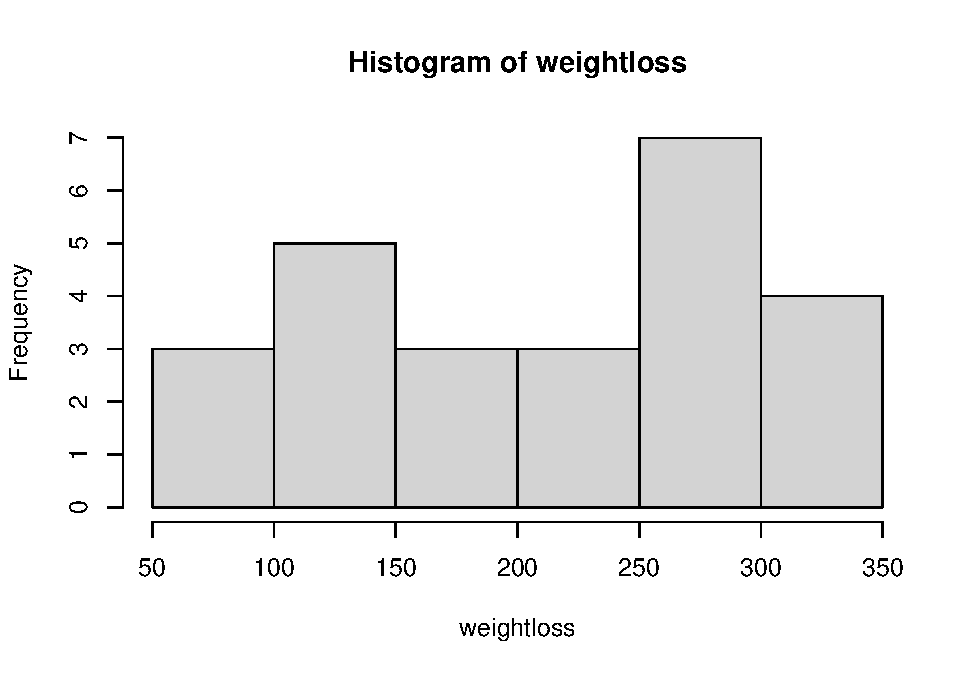
\includegraphics{phcm9795-solutions-R_files/figure-latex/unnamed-chunk-3-1.pdf}

\begin{Shaded}
\begin{Highlighting}[]
\CommentTok{\# The default values look ok, so let\textquotesingle{}s add labels and titles}
\FunctionTok{hist}\NormalTok{(weightloss, }\AttributeTok{xlab=}\StringTok{"Weight loss (g)"}\NormalTok{, }\AttributeTok{main=}\StringTok{"Weight loss for 25 participants"}\NormalTok{)}
\end{Highlighting}
\end{Shaded}

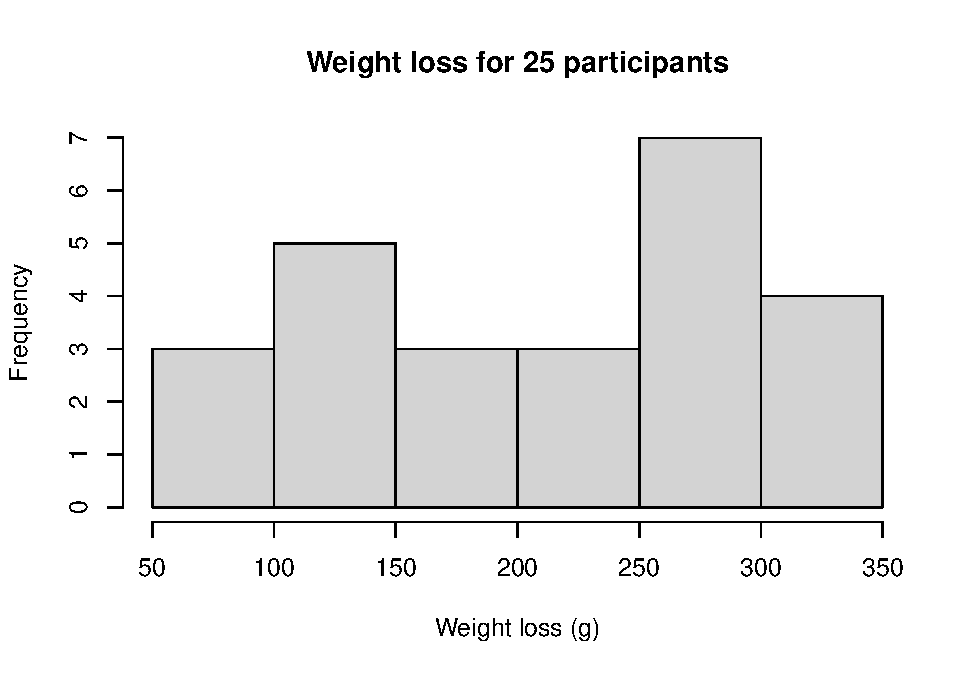
\includegraphics{phcm9795-solutions-R_files/figure-latex/unnamed-chunk-3-2.pdf}

Note that the question requests \textbf{relative frequencies}, so we can use the code in Section 1.12 to amend this graph:

\begin{Shaded}
\begin{Highlighting}[]
\NormalTok{h }\OtherTok{\textless{}{-}} \FunctionTok{hist}\NormalTok{(weightloss, }\AttributeTok{plot=}\ConstantTok{FALSE}\NormalTok{)}
\NormalTok{h}\SpecialCharTok{$}\NormalTok{density }\OtherTok{\textless{}{-}}\NormalTok{ h}\SpecialCharTok{$}\NormalTok{counts}\SpecialCharTok{/}\FunctionTok{sum}\NormalTok{(h}\SpecialCharTok{$}\NormalTok{counts)}\SpecialCharTok{*}\DecValTok{100}
\FunctionTok{plot}\NormalTok{(h, }\AttributeTok{freq=}\ConstantTok{FALSE}\NormalTok{, }
     \AttributeTok{xlab=}\StringTok{"Weight loss (g)"}\NormalTok{, }
     \AttributeTok{ylab=}\StringTok{"Relative frequency (\%)"}\NormalTok{,}
     \AttributeTok{main=}\StringTok{"Fig 1.1: Weight loss for 25 participants"}\NormalTok{)}
\end{Highlighting}
\end{Shaded}

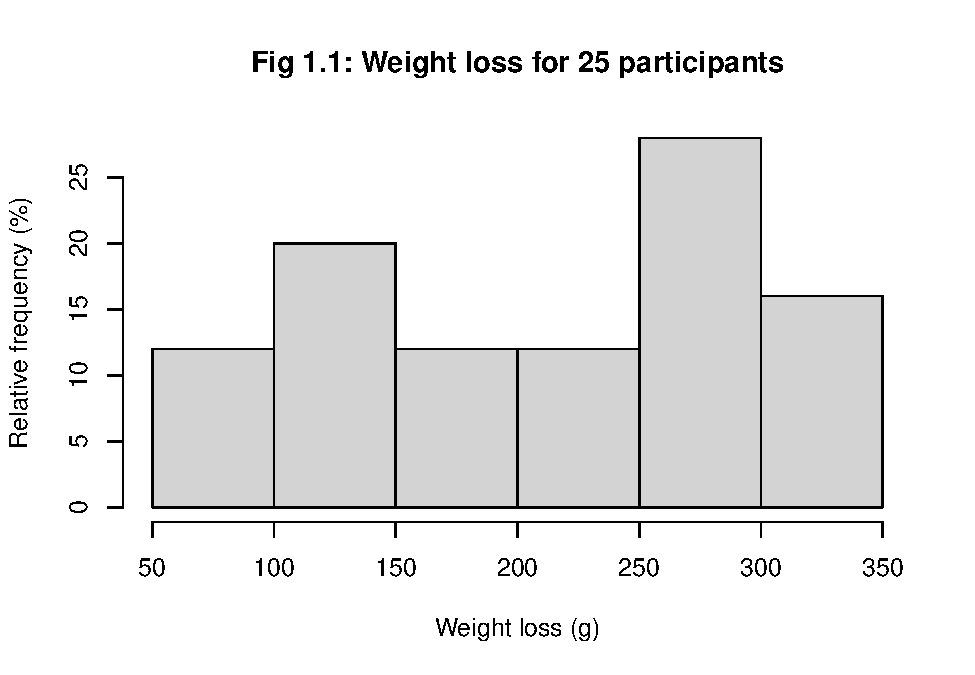
\includegraphics{phcm9795-solutions-R_files/figure-latex/unnamed-chunk-4-1.pdf}

\hypertarget{activity-1.2}{%
\subsection*{Activity 1.2}\label{activity-1.2}}
\addcontentsline{toc}{subsection}{Activity 1.2}

Researchers at a maternity hospital in the 1970s conducted a study of low birth weight babies. Low birth weight is classified as a weight of 2,500g or less at birth. Data were collected on age and smoking status of mothers and the birth weight of their babies. The file \texttt{Activity\_S1.2.rds} contains data on the participants in the study. The file is located on Moodle in the Learning Activities section.

Use R to create a 2 by 2 table to show the proportions of low birth weight babies born to mothers who smoked during pregnancy and those that did not smoke during pregnancy.

\begin{Shaded}
\begin{Highlighting}[]
\FunctionTok{library}\NormalTok{(jmv)}

\NormalTok{babies }\OtherTok{\textless{}{-}}\FunctionTok{readRDS}\NormalTok{(}\StringTok{"data/activities/Activity\_S1.2.rds"}\NormalTok{)}

\CommentTok{\# Examine the first six rows of data}
\FunctionTok{head}\NormalTok{(babies)}
\end{Highlighting}
\end{Shaded}

\begin{verbatim}
##   AGE    AgeGrp  BWT                 LOW SMOKE
## 1  14 <20 years 2466    Low birth weight   Yes
## 2  14 <20 years 2495    Low birth weight    No
## 3  14 <20 years 3941 Normal birth weight    No
## 4  15 <20 years 2353    Low birth weight    No
## 5  15 <20 years 2381    Low birth weight    No
## 6  15 <20 years 2778 Normal birth weight    No
\end{verbatim}

\begin{Shaded}
\begin{Highlighting}[]
\CommentTok{\# Create a two{-}way table showing row percents}
\FunctionTok{contTables}\NormalTok{(}\AttributeTok{data=}\NormalTok{babies, }\AttributeTok{rows=}\NormalTok{SMOKE, }\AttributeTok{cols=}\NormalTok{LOW, }\AttributeTok{pcRow=}\ConstantTok{TRUE}\NormalTok{)}
\end{Highlighting}
\end{Shaded}

\begin{verbatim}
## 
##  CONTINGENCY TABLES
## 
##  Contingency Tables                                                                
##  ───────────────────────────────────────────────────────────────────────────────── 
##    SMOKE                    Low birth weight    Normal birth weight    Total       
##  ───────────────────────────────────────────────────────────────────────────────── 
##    Yes      Observed                      30                     44           74   
##             % within row            40.54054               59.45946    100.00000   
##                                                                                    
##    No       Observed                      29                     86          115   
##             % within row            25.21739               74.78261    100.00000   
##                                                                                    
##    Total    Observed                      59                    130          189   
##             % within row            31.21693               68.78307    100.00000   
##  ───────────────────────────────────────────────────────────────────────────────── 
## 
## 
##  χ² Tests                              
##  ───────────────────────────────────── 
##          Value       df    p           
##  ───────────────────────────────────── 
##    χ²    4.923705     1    0.0264906   
##    N          189                      
##  ─────────────────────────────────────
\end{verbatim}

Answer the following questions:

\begin{enumerate}
\def\labelenumi{\alph{enumi})}
\tightlist
\item
  What was the total number of mothers who smoked during pregnancy?
\end{enumerate}

\begin{quote}
There were 74 mothers who smoked during pregancy.
\end{quote}

\begin{enumerate}
\def\labelenumi{\alph{enumi})}
\setcounter{enumi}{1}
\tightlist
\item
  What proportion of mothers who smoked gave birth to low birth weight babies? What proportion of non-smoking mothers gave birth to low birth weight babies?
\end{enumerate}

\begin{quote}
41\% of mothers who smoked and 25\% of non-smoking mothers gave birth to low birth weight babies.
\end{quote}

\begin{enumerate}
\def\labelenumi{\alph{enumi})}
\setcounter{enumi}{2}
\tightlist
\item
  Use R to construct a stacked bar chart of the data to examine if there a difference in the proportion of babies born with a low birth weight in relation to mother's age? Provide appropriate labels for the axes and give the graph an appropriate title.
\end{enumerate}

\begin{quote}
We follow the instructions for creating a stacked bar chart in Module 1. First we create a table of low birth weight by mothers' age-group, and create a stacked bar chart (to check that we're on the right track):
\end{quote}

\begin{Shaded}
\begin{Highlighting}[]
\NormalTok{counts }\OtherTok{\textless{}{-}} \FunctionTok{table}\NormalTok{(babies}\SpecialCharTok{$}\NormalTok{LOW, babies}\SpecialCharTok{$}\NormalTok{AgeGrp)}
\NormalTok{counts}
\end{Highlighting}
\end{Shaded}

\begin{verbatim}
##                      
##                       <20 years 20-24 years 25-29 years 30-34 years
##   Low birth weight           15          25          15           4
##   Normal birth weight        36          44          27          18
##                      
##                       35 or more years
##   Low birth weight                   0
##   Normal birth weight                5
\end{verbatim}

\begin{Shaded}
\begin{Highlighting}[]
\FunctionTok{barplot}\NormalTok{(counts, }
        \AttributeTok{main=}\StringTok{"Fig 1.2: Frequency of low birth weight by mother\textquotesingle{}s age group"}\NormalTok{,}
        \AttributeTok{legend =} \FunctionTok{rownames}\NormalTok{(counts), }\AttributeTok{beside=}\ConstantTok{FALSE}\NormalTok{)}
\end{Highlighting}
\end{Shaded}

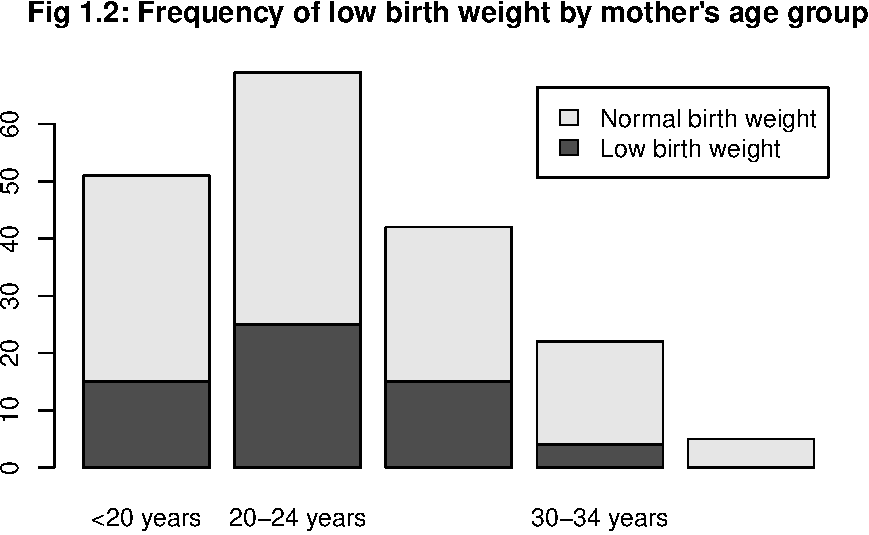
\includegraphics{phcm9795-solutions-R_files/figure-latex/unnamed-chunk-7-1.pdf}

\begin{quote}
We then calculate the \emph{relative frequency} of low-birth weight by mothers' age group
\end{quote}

\begin{Shaded}
\begin{Highlighting}[]
\NormalTok{percent }\OtherTok{\textless{}{-}} \FunctionTok{prop.table}\NormalTok{(counts, }\AttributeTok{margin=}\DecValTok{2}\NormalTok{)}\SpecialCharTok{*}\DecValTok{100}
\NormalTok{percent}
\end{Highlighting}
\end{Shaded}

\begin{verbatim}
##                      
##                       <20 years 20-24 years 25-29 years 30-34 years
##   Low birth weight     29.41176    36.23188    35.71429    18.18182
##   Normal birth weight  70.58824    63.76812    64.28571    81.81818
##                      
##                       35 or more years
##   Low birth weight             0.00000
##   Normal birth weight        100.00000
\end{verbatim}

\begin{quote}
and use the \texttt{barplot()} command, as per the notes:
\end{quote}

\begin{Shaded}
\begin{Highlighting}[]
\FunctionTok{barplot}\NormalTok{(percent, }
        \AttributeTok{main=}\StringTok{"Fig 1.3: Relative frequency of low birth weight by mother\textquotesingle{}s age group"}\NormalTok{,}
        \AttributeTok{legend =} \FunctionTok{rownames}\NormalTok{(percent), }\AttributeTok{beside=}\ConstantTok{FALSE}\NormalTok{)}
\end{Highlighting}
\end{Shaded}

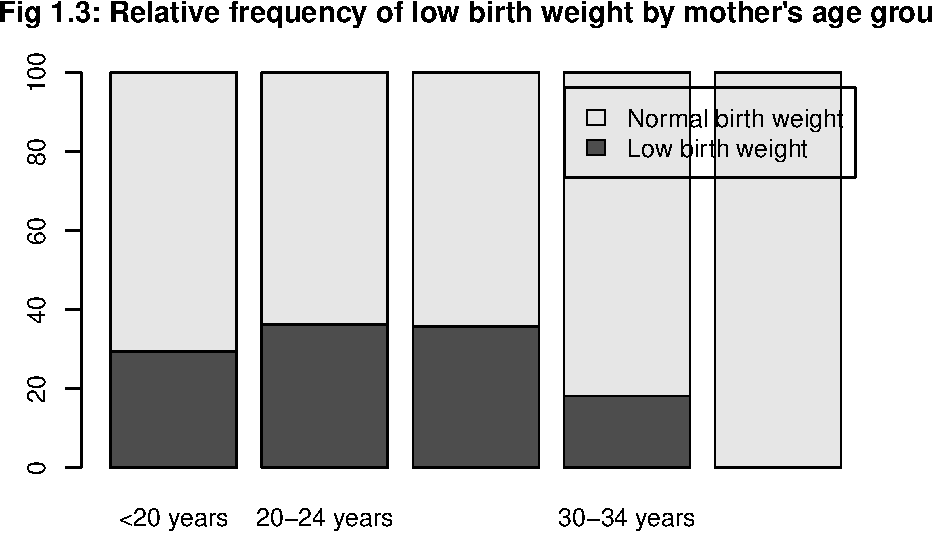
\includegraphics{phcm9795-solutions-R_files/figure-latex/unnamed-chunk-9-1.pdf}

\begin{enumerate}
\def\labelenumi{\alph{enumi})}
\setcounter{enumi}{3}
\tightlist
\item
  Using your answers to the question a) and b), write a brief conclusion about the relationship of low birth weight and mother's age and smoking status.
\end{enumerate}

\begin{quote}
In the study, the greatest number of babies were born to mothers in the 20-24 years age group, with the number of babies born declining with increasing maternal age for mothers older than 20-24 years (Figure 1.2). A larger proportion of mothers in the \textless20 years, 20-24 years and 25-29 years age groups gave birth to low birth weight babies compared to mothers aged 30-34 years. No low birth weight babies were born to mothers aged 35 or more (Figure 1.3).
\end{quote}

\begin{quote}
A larger proportion of mothers who smoked during pregnancy gave birth to low birth weight babies compared to mothers who did not smoke during pregnancy.
\end{quote}

\begin{quote}
NB: You will revisit two-way tables in Module 7 where you will conduct statistical tests to determine if the proportions are statistically different to each other.
\end{quote}

\textbf{Note: } Coding graphs, particularly clustered and stacked bar graphs can be difficult! The site \url{https://r-graph-gallery.com/} gives excellent instructions on constructing different types of graphs in R.

\hypertarget{activity-1.3}{%
\subsection*{Activity 1.3}\label{activity-1.3}}
\addcontentsline{toc}{subsection}{Activity 1.3}

Using R, estimate the mean, median, mode, standard deviation, range and interquartile range for the data Activity\_S1.3.rds, available on Moodle.

\begin{Shaded}
\begin{Highlighting}[]
\NormalTok{act1\_3 }\OtherTok{\textless{}{-}} \FunctionTok{readRDS}\NormalTok{(}\StringTok{"data/activities/Activity\_S1.3.rds"}\NormalTok{)}

\FunctionTok{descriptives}\NormalTok{(act1\_3, }\AttributeTok{mode=}\ConstantTok{TRUE}\NormalTok{, }\AttributeTok{iqr=}\ConstantTok{TRUE}\NormalTok{, }\AttributeTok{pc=}\ConstantTok{TRUE}\NormalTok{)}
\end{Highlighting}
\end{Shaded}

\begin{verbatim}
## 
##  DESCRIPTIVES
## 
##  Descriptives                         
##  ──────────────────────────────────── 
##                          Lead_concn   
##  ──────────────────────────────────── 
##    N                             15   
##    Missing                        0   
##    Mean                    1.500000   
##    Median                  1.500000   
##    Mode                    1.900000   
##    Standard deviation     0.8434623   
##    IQR                    1.0000000   
##    Minimum                0.1000000   
##    Maximum                 3.200000   
##    25th percentile        0.9500000   
##    50th percentile         1.500000   
##    75th percentile         1.950000   
##  ────────────────────────────────────
\end{verbatim}

\begin{quote}
We can use the \texttt{descriptives()} function to obtain summary statistics. Examining the help entry for \texttt{descriptives()} shows we can request the mode using \texttt{mode=TRUE}, the interquartile range using \texttt{iqr=TRUE} and the percentiles (by default, the quartiles) using \texttt{pc=TRUE}.
The mean is estimated as 1.50, the median is 1.5 and the mode is 1.9. The standard deviation is estimated as 0.843, the range is from 0.1 to 3.2, and the inter-quartile range is from 1.0 to 2.0 (both rounded to 1 decimal place).
\end{quote}

\begin{quote}
Note: no units were provided for the data used in this question. Summary statistics must be presented with their units where the units are available.
\end{quote}

\hypertarget{activity-1.4}{%
\subsection*{Activity 1.4}\label{activity-1.4}}
\addcontentsline{toc}{subsection}{Activity 1.4}

Data of diastolic blood pressure (BP) of a sample of study participants are provided in the dataset Activity\_S1.4.rds. Compute the mean, median, range and SD of diastolic BP.

\begin{Shaded}
\begin{Highlighting}[]
\NormalTok{act1\_4 }\OtherTok{\textless{}{-}} \FunctionTok{readRDS}\NormalTok{(}\StringTok{"data/activities/Activity\_S1.4.rds"}\NormalTok{)}

\FunctionTok{descriptives}\NormalTok{(act1\_4)}
\end{Highlighting}
\end{Shaded}

\begin{verbatim}
## 
##  DESCRIPTIVES
## 
##  Descriptives                       
##  ────────────────────────────────── 
##                          diabp      
##  ────────────────────────────────── 
##    N                          100   
##    Missing                      0   
##    Mean                  82.23000   
##    Median                83.00000   
##    Standard deviation    13.01522   
##    Minimum               56.00000   
##    Maximum               118.0000   
##  ──────────────────────────────────
\end{verbatim}

\begin{quote}
The mean is 82.2 mmHg and the median is 83.0 mmHg. The range is 56.0 to 118.0 mmHg (62.0 mmHg) and the standard deviation is 13.02 mmHg.
\end{quote}

\begin{quote}
\emph{Note that the original data have one decimal place, so we can report the median with one decimal place. Although we are justified in presenting the mean to two decimal places (1 extra than the original data), and the standard deviation with three decimal places (1 more than the mean), there is little to be gained in this level of precision when presenting summary statistics for blood pressure.}
\end{quote}

\hypertarget{activity-1.5}{%
\subsection*{Activity 1.5}\label{activity-1.5}}
\addcontentsline{toc}{subsection}{Activity 1.5}

In a study of 100 participants data were missing for 5 people. The missing data points were coded as `99'. The mean of the data was estimated as 45.0 with a standard deviation of 5.6; the smallest and greatest values are 16 and 65 respectively.

If the researcher analysed the data as if the 99s were real data, would it make the following statistics larger, smaller, or stay the same?

\begin{enumerate}
\def\labelenumi{\alph{enumi})}
\tightlist
\item
  Mean
\end{enumerate}

\begin{quote}
The mean will be larger.
\end{quote}

\begin{enumerate}
\def\labelenumi{\alph{enumi})}
\setcounter{enumi}{1}
\tightlist
\item
  Standard Deviation
\end{enumerate}

\begin{quote}
The standard deviation will be larger.
\end{quote}

\begin{enumerate}
\def\labelenumi{\alph{enumi})}
\setcounter{enumi}{2}
\tightlist
\item
  Range
\end{enumerate}

\begin{quote}
The range will be larger. The smallest value is still 16, but the largest is 99, and so the range is 99 − 16 = 83.
\end{quote}

\hypertarget{activity-1.6}{%
\subsection*{Activity 1.6}\label{activity-1.6}}
\addcontentsline{toc}{subsection}{Activity 1.6}

Which of the following statements are true? The more dispersed, or spread out, a set of observations are:

\begin{enumerate}
\def\labelenumi{\alph{enumi})}
\tightlist
\item
  The smaller the mean value
\end{enumerate}

\begin{quote}
This is not true because the mean is not influenced by the spread of the values (if the distribution is symmetrical around the mean value)
\end{quote}

\begin{enumerate}
\def\labelenumi{\alph{enumi})}
\setcounter{enumi}{1}
\tightlist
\item
  The larger the standard deviation
\end{enumerate}

\begin{quote}
This is true. The larger the spread, the larger the deviations from the mean. Hence the standard deviation will be larger.
\end{quote}

\begin{enumerate}
\def\labelenumi{\alph{enumi})}
\setcounter{enumi}{2}
\tightlist
\item
  The smaller the variance
\end{enumerate}

\begin{quote}
This is not true. The variance will be larger if the deviations from the mean are larger.
\end{quote}

\hypertarget{activity-1.7}{%
\subsection*{Activity 1.7}\label{activity-1.7}}
\addcontentsline{toc}{subsection}{Activity 1.7}

If the variance for a set of scores is equal to 9, what is the standard deviation?

\begin{quote}
SD = \(\sqrt{variance} = \sqrt{9} = 3\).
\end{quote}

\hypertarget{module-1-full-script}{%
\chapter*{Module 1: Full script}\label{module-1-full-script}}
\addcontentsline{toc}{chapter}{Module 1: Full script}

\begin{Shaded}
\begin{Highlighting}[]
\CommentTok{\# Author: Timothy Dobbins}
\CommentTok{\# Date: May, 2022}
\CommentTok{\# Purpose: Learning activities for Module 1}

\FunctionTok{library}\NormalTok{(jmv)}

\DocumentationTok{\#\#\# Activity 1.1}

\NormalTok{weightloss }\OtherTok{\textless{}{-}} \FunctionTok{c}\NormalTok{(}\DecValTok{255}\NormalTok{, }\DecValTok{198}\NormalTok{, }\DecValTok{283}\NormalTok{, }\DecValTok{312}\NormalTok{, }\DecValTok{283}\NormalTok{, }\DecValTok{57}\NormalTok{,  }\DecValTok{85}\NormalTok{, }\DecValTok{312}\NormalTok{, }\DecValTok{142}\NormalTok{, }\DecValTok{113}\NormalTok{,}
                \DecValTok{227}\NormalTok{, }\DecValTok{283}\NormalTok{, }\DecValTok{255}\NormalTok{, }\DecValTok{340}\NormalTok{, }\DecValTok{142}\NormalTok{, }\DecValTok{113}\NormalTok{, }\DecValTok{312}\NormalTok{, }\DecValTok{227}\NormalTok{,  }\DecValTok{85}\NormalTok{, }\DecValTok{170}\NormalTok{,}
                \DecValTok{255}\NormalTok{, }\DecValTok{198}\NormalTok{, }\DecValTok{113}\NormalTok{, }\DecValTok{227}\NormalTok{, }\DecValTok{255}\NormalTok{)}
\CommentTok{\# Check the default histogram:}
\FunctionTok{hist}\NormalTok{(weightloss)}

\CommentTok{\# The default values look ok, so let\textquotesingle{}s add labels and titles}
\FunctionTok{hist}\NormalTok{(weightloss, }\AttributeTok{xlab=}\StringTok{"Weight loss (g)"}\NormalTok{, }\AttributeTok{main=}\StringTok{"Weight loss for 25 participants"}\NormalTok{)}

\CommentTok{\# Construct a relative frequency histogram}
\NormalTok{h }\OtherTok{\textless{}{-}} \FunctionTok{hist}\NormalTok{(weightloss, }\AttributeTok{plot=}\ConstantTok{FALSE}\NormalTok{)}
\NormalTok{h}\SpecialCharTok{$}\NormalTok{density }\OtherTok{\textless{}{-}}\NormalTok{ h}\SpecialCharTok{$}\NormalTok{counts}\SpecialCharTok{/}\FunctionTok{sum}\NormalTok{(h}\SpecialCharTok{$}\NormalTok{counts)}\SpecialCharTok{*}\DecValTok{100}
\FunctionTok{plot}\NormalTok{(h, }\AttributeTok{freq=}\ConstantTok{FALSE}\NormalTok{, }
     \AttributeTok{xlab=}\StringTok{"Weight loss (g)"}\NormalTok{, }
     \AttributeTok{ylab=}\StringTok{"Relative frequency (\%)"}\NormalTok{,}
     \AttributeTok{main=}\StringTok{"Fig 1.1: Weight loss for 25 participants"}\NormalTok{)}


\DocumentationTok{\#\#\# Activity 1.2}
\NormalTok{babies }\OtherTok{\textless{}{-}}\FunctionTok{readRDS}\NormalTok{(}\StringTok{"data/activities/Activity\_S1.2.rds"}\NormalTok{)}

\CommentTok{\# Examine the first six rows of data}
\FunctionTok{head}\NormalTok{(babies)}

\CommentTok{\# Create a two{-}way table showing row percents}
\FunctionTok{contTables}\NormalTok{(}\AttributeTok{data=}\NormalTok{babies, }\AttributeTok{rows=}\NormalTok{SMOKE, }\AttributeTok{cols=}\NormalTok{LOW, }\AttributeTok{pcRow=}\ConstantTok{TRUE}\NormalTok{)}

\CommentTok{\# Construct bar charts}
\NormalTok{counts }\OtherTok{\textless{}{-}} \FunctionTok{table}\NormalTok{(babies}\SpecialCharTok{$}\NormalTok{LOW, babies}\SpecialCharTok{$}\NormalTok{AgeGrp)}
\NormalTok{counts}

\FunctionTok{barplot}\NormalTok{(counts, }
        \AttributeTok{main=}\StringTok{"Fig 1.2: Frequency of low birt weight by mother\textquotesingle{}s age group"}\NormalTok{,}
        \AttributeTok{legend =} \FunctionTok{rownames}\NormalTok{(counts), }\AttributeTok{beside=}\ConstantTok{FALSE}\NormalTok{)}

\NormalTok{percent }\OtherTok{\textless{}{-}} \FunctionTok{prop.table}\NormalTok{(counts, }\AttributeTok{margin=}\DecValTok{2}\NormalTok{)}\SpecialCharTok{*}\DecValTok{100}
\NormalTok{percent}

\FunctionTok{barplot}\NormalTok{(percent, }
        \AttributeTok{main=}\StringTok{"Fig 1.3: Relative frequency of low birth weight by mother\textquotesingle{}s age group"}\NormalTok{,}
        \AttributeTok{legend =} \FunctionTok{rownames}\NormalTok{(percent), }\AttributeTok{beside=}\ConstantTok{FALSE}\NormalTok{)}


\DocumentationTok{\#\#\# Activity 1.3}

\NormalTok{act1\_3 }\OtherTok{\textless{}{-}} \FunctionTok{readRDS}\NormalTok{(}\StringTok{"data/activities/Activity\_S1.3.rds"}\NormalTok{)}

\FunctionTok{descriptives}\NormalTok{(act1\_3, }\AttributeTok{mode=}\ConstantTok{TRUE}\NormalTok{, }\AttributeTok{iqr=}\ConstantTok{TRUE}\NormalTok{, }\AttributeTok{pc=}\ConstantTok{TRUE}\NormalTok{)}


\DocumentationTok{\#\#\# Activity 1.4}

\NormalTok{act1\_4 }\OtherTok{\textless{}{-}} \FunctionTok{readRDS}\NormalTok{(}\StringTok{"data/activities/Activity\_S1.4.rds"}\NormalTok{)}

\FunctionTok{descriptives}\NormalTok{(act1\_4)}
\end{Highlighting}
\end{Shaded}

\hypertarget{module-2-solutions-to-learning-activities}{%
\chapter*{Module 2: Solutions to Learning Activities}\label{module-2-solutions-to-learning-activities}}
\addcontentsline{toc}{chapter}{Module 2: Solutions to Learning Activities}

\hypertarget{activity-2.1}{%
\subsection*{Activity 2.1}\label{activity-2.1}}
\addcontentsline{toc}{subsection}{Activity 2.1}

In a Randomised Controlled Trial, the preference of a new drug was tested against an established drug by giving both drugs to each of 90 people. Assume that the two drugs are equally preferred, that is, the probability that a patient prefers either of the drugs is equal (50\%). Use one of the binomial functions in R to compute the probability that 60 or more patients would prefer the new drug. In completing this question, determine:

\begin{enumerate}
\def\labelenumi{\alph{enumi})}
\tightlist
\item
  The number of trials (n)
\end{enumerate}

\begin{quote}
Here, each participant represents a `trial', so n is 90.
\end{quote}

\begin{enumerate}
\def\labelenumi{\alph{enumi})}
\setcounter{enumi}{1}
\tightlist
\item
  The number of successes we are interested in (k)
\end{enumerate}

\begin{quote}
We are interested in determining the probability that 60 or more participants prefer the new drug, so k is 60.
\end{quote}

\begin{enumerate}
\def\labelenumi{\alph{enumi})}
\setcounter{enumi}{2}
\tightlist
\item
  The probability of success for each trial (p)
\end{enumerate}

\begin{quote}
We are told to assume that the two drugs are equally preferred, so p is 0.5.
\end{quote}

\begin{enumerate}
\def\labelenumi{\alph{enumi})}
\setcounter{enumi}{3}
\tightlist
\item
  The form of the R function: dbinom or pbinom
\end{enumerate}

\begin{quote}
We need to calculate the probability that 60 or more participants prefer the new drug. The two R functions can be interpreted as follows:
- the \texttt{dbinom} function gives the probability of observing 60 successes;
- the \texttt{pbinom} function gives the probability of observing 60 or fewer successes;
- the \texttt{pbinom} function with \texttt{lower.tail=FALSE} gives the probability of observing \emph{more than} 60 successes.
\end{quote}

\begin{quote}
We therefore want to use \texttt{pbinom} function with \texttt{lower.tail=FALSE} here.
\end{quote}

\begin{enumerate}
\def\labelenumi{\alph{enumi})}
\setcounter{enumi}{4}
\tightlist
\item
  The final probability.
\end{enumerate}

\begin{quote}
To calculate the probability of obtaining 60 or more successes, we need to calculate the probabibility of observing \emph{more than} 59 successes. So the function we use is:
\end{quote}

\begin{Shaded}
\begin{Highlighting}[]
\FunctionTok{pbinom}\NormalTok{(}\AttributeTok{q=}\DecValTok{59}\NormalTok{, }\AttributeTok{size=}\DecValTok{90}\NormalTok{, }\AttributeTok{prob=}\FloatTok{0.5}\NormalTok{, }\AttributeTok{lower.tail =} \ConstantTok{FALSE}\NormalTok{)}
\end{Highlighting}
\end{Shaded}

\begin{verbatim}
## [1] 0.001030133
\end{verbatim}

\begin{quote}
Therefore, the probability that 60 or more patients would prefer the new drug is 0.001 or 0.1\%.
\end{quote}

\hypertarget{activity-2.2}{%
\subsection*{Activity 2.2}\label{activity-2.2}}
\addcontentsline{toc}{subsection}{Activity 2.2}

A case of Schistosomiasis is identified by the detection of schistosome ova in a faecal sample. In patients with a low level of infection, a field technique of faecal examination has a probability of 0.35 of detecting ova in any one faecal sample. If five samples are routinely examined for each patient, use R to compute the probability that a patient with a low level of infection:

\begin{enumerate}
\def\labelenumi{\alph{enumi})}
\tightlist
\item
  Will not be identified?
\end{enumerate}

\begin{quote}
In all of these questions, \texttt{size} is 5 and \texttt{prob} is 0.35. Here we need to calculate the probability of P(X=0), and we can use the \texttt{dbinom} function:
\end{quote}

\begin{Shaded}
\begin{Highlighting}[]
\FunctionTok{dbinom}\NormalTok{(}\AttributeTok{x=}\DecValTok{0}\NormalTok{, }\AttributeTok{size=}\DecValTok{5}\NormalTok{, }\AttributeTok{prob=}\FloatTok{0.35}\NormalTok{)}
\end{Highlighting}
\end{Shaded}

\begin{verbatim}
## [1] 0.1160291
\end{verbatim}

\begin{quote}
The probability P(X=0) = 0.116 or 11.6\%.
\end{quote}

\begin{enumerate}
\def\labelenumi{\alph{enumi})}
\setcounter{enumi}{1}
\tightlist
\item
  Will be identified in two of the samples?
\end{enumerate}

\begin{quote}
The probability P(X=2)= 0. 336 or 33.6\%:
\end{quote}

\begin{Shaded}
\begin{Highlighting}[]
\FunctionTok{dbinom}\NormalTok{(}\AttributeTok{x=}\DecValTok{2}\NormalTok{, }\AttributeTok{size=}\DecValTok{5}\NormalTok{, }\AttributeTok{prob=}\FloatTok{0.35}\NormalTok{)}
\end{Highlighting}
\end{Shaded}

\begin{verbatim}
## [1] 0.3364156
\end{verbatim}

\begin{enumerate}
\def\labelenumi{\alph{enumi})}
\setcounter{enumi}{2}
\tightlist
\item
  Will be identified in all the samples?
\end{enumerate}

The probability P(X=5) = .005 or 0.5\%:

\begin{Shaded}
\begin{Highlighting}[]
\FunctionTok{dbinom}\NormalTok{(}\AttributeTok{x=}\DecValTok{5}\NormalTok{, }\AttributeTok{size=}\DecValTok{5}\NormalTok{, }\AttributeTok{prob=}\FloatTok{0.35}\NormalTok{)}
\end{Highlighting}
\end{Shaded}

\begin{verbatim}
## [1] 0.005252187
\end{verbatim}

\begin{enumerate}
\def\labelenumi{\alph{enumi})}
\setcounter{enumi}{3}
\tightlist
\item
  Will be identified in at most 3 of the samples?
\end{enumerate}

\begin{quote}
``At most 3 samples'' is the same as 3 or fewer samples, so we can use the pbinom function. The probability P(X≤3) = .946 or 94.6\%:
\end{quote}

\begin{Shaded}
\begin{Highlighting}[]
\FunctionTok{pbinom}\NormalTok{(}\AttributeTok{q=}\DecValTok{3}\NormalTok{, }\AttributeTok{size=}\DecValTok{5}\NormalTok{, }\AttributeTok{prob=}\FloatTok{0.35}\NormalTok{)}
\end{Highlighting}
\end{Shaded}

\begin{verbatim}
## [1] 0.9459775
\end{verbatim}

\hypertarget{activity-2.3}{%
\subsection*{Activity 2.3}\label{activity-2.3}}
\addcontentsline{toc}{subsection}{Activity 2.3}

If weights of men are Normally distributed with a population mean \(\mu\) = 87, and a population standard deviation, \(\sigma\) = 8 kg:

\begin{enumerate}
\def\labelenumi{\alph{enumi})}
\tightlist
\item
  What is the probability that a man will weigh 95 kg or more? Draw a Normal curve of the area represented by this probability in the population (i.e.~with \(\mu\) = 87 kg and \(\sigma\) = 8 kg).
\end{enumerate}

\begin{quote}
The curve representing the desired probability is drawn below, with the region above 95kg shaded to represent the probability of interest. Note that this curve was generated by a computer: a hand-drawn figure is completely acceptable. A hand-drawn figure will probably look much less tidy, but the main thing to notice is that the shaded area looks like it would represent less than 50\% of the total curve. Therefore, our final probability should be less than 0.5.
\end{quote}

\begin{figure}
\centering
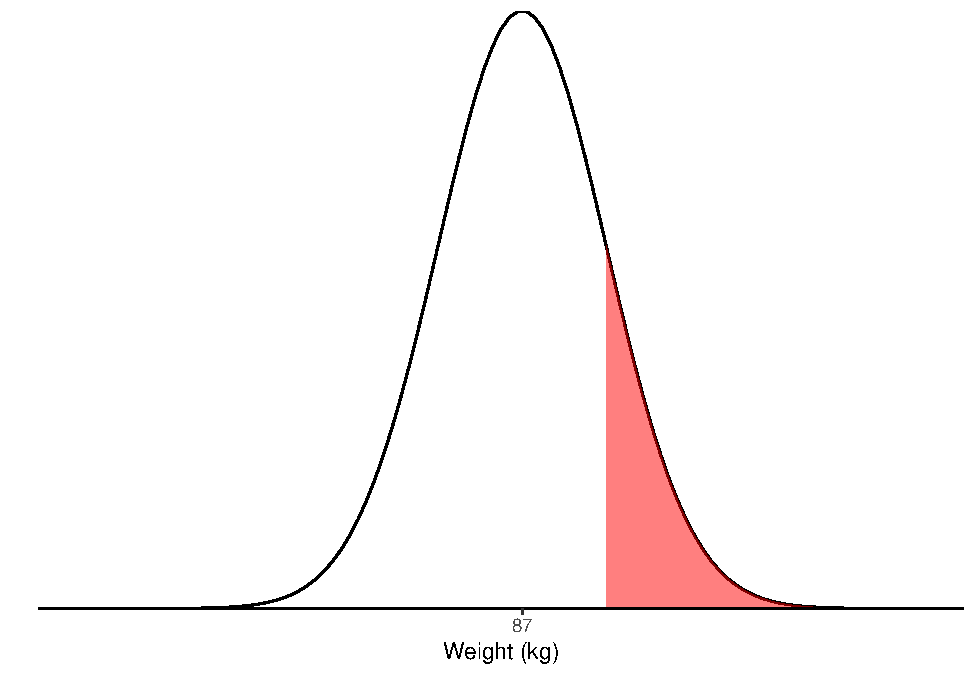
\includegraphics{phcm9795-solutions-R_files/figure-latex/unnamed-chunk-18-1.pdf}
\caption{\label{fig:unnamed-chunk-18}Probability that a man will weigh 95kg or more}
\end{figure}

\begin{quote}
The probability is calculated as:
\end{quote}

\begin{Shaded}
\begin{Highlighting}[]
\CommentTok{\# Probability:}
\FunctionTok{pnorm}\NormalTok{(}\DecValTok{95}\NormalTok{, }\AttributeTok{mean=}\DecValTok{87}\NormalTok{, }\AttributeTok{sd=}\DecValTok{8}\NormalTok{, }\AttributeTok{lower.tail=}\ConstantTok{FALSE}\NormalTok{)}
\end{Highlighting}
\end{Shaded}

\begin{verbatim}
## [1] 0.1586553
\end{verbatim}

\begin{quote}
Therefore, the probability that a man from this population weighs 95 kg or more is 0.16 or 16\%.
\end{quote}

\begin{enumerate}
\def\labelenumi{\alph{enumi})}
\setcounter{enumi}{1}
\tightlist
\item
  What is the probability that a man will weigh more than 75 kg but less than 95 kg? Draw the area represented by this probability on a standardised Normal curve.
\end{enumerate}

\begin{quote}
The curve to represent this probability is shown below. To obtain the probability represented by the shaded region, we again use the fact that the total area under a Normal curve must add to 1. Let's break the curve into three parts, which we will call A, B and C.
\end{quote}

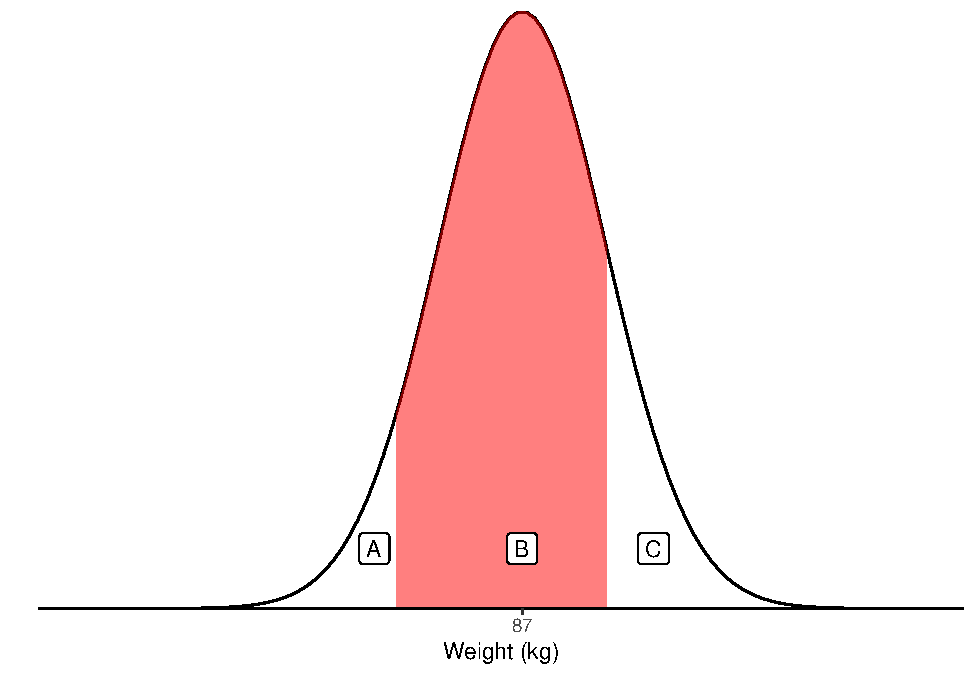
\includegraphics{phcm9795-solutions-R_files/figure-latex/unnamed-chunk-20-1.pdf}

\begin{quote}
We use that fact that A+B+C=1 to derive that B = 1-- A -- C. We have already calculated C in Part (a) of this question. To calculate A:
\end{quote}

\begin{Shaded}
\begin{Highlighting}[]
\FunctionTok{pnorm}\NormalTok{(}\DecValTok{75}\NormalTok{, }\AttributeTok{mean=}\DecValTok{87}\NormalTok{, }\AttributeTok{sd=}\DecValTok{8}\NormalTok{, }\AttributeTok{lower.tail=}\ConstantTok{TRUE}\NormalTok{)}
\end{Highlighting}
\end{Shaded}

\begin{verbatim}
## [1] 0.0668072
\end{verbatim}

P(Weight \textless{} 75) = 0.0668.

\begin{quote}
The region B is calculated as: 1 - 0.1587 - 0.0668 = 0.7745.
\end{quote}

\begin{quote}
So the probability that a man will weigh more than 75 kg but less than 95 kg is 0.77, or 77\%.
\end{quote}

\hypertarget{activity-2.4}{%
\subsection*{Activity 2.4}\label{activity-2.4}}
\addcontentsline{toc}{subsection}{Activity 2.4}

Using the health survey data described in the R notes of this module, create a new variable, BMI, which is equal to a person's weight (in kg) divided by their height (in metres) squared (i.e.~\(\text{BMI} = \frac{\text{weight (kg)}}{\text{[height (m)]}^2}\). Categorise BMI using the WHO categories provided in the R notes. Create a two-way table to display the distribution of BMI categories by sex (sex: 1 = respondent identifies as male; 2 = respondent identifies as female). Does there appear to be a difference in categorised BMI between males and females?

\begin{Shaded}
\begin{Highlighting}[]
\FunctionTok{library}\NormalTok{(readxl)}
\FunctionTok{library}\NormalTok{(jmv)}

\NormalTok{survey }\OtherTok{\textless{}{-}} \FunctionTok{read\_excel}\NormalTok{(}\StringTok{"data/examples/health{-}survey.xlsx"}\NormalTok{)}
\FunctionTok{summary}\NormalTok{(survey)}
\end{Highlighting}
\end{Shaded}

\begin{verbatim}
##       sex           height          weight      
##  Min.   :1.00   Min.   :1.220   Min.   : 22.70  
##  1st Qu.:1.00   1st Qu.:1.630   1st Qu.: 68.00  
##  Median :2.00   Median :1.700   Median : 79.40  
##  Mean   :1.55   Mean   :1.698   Mean   : 81.19  
##  3rd Qu.:2.00   3rd Qu.:1.780   3rd Qu.: 90.70  
##  Max.   :2.00   Max.   :2.010   Max.   :213.20
\end{verbatim}

\begin{quote}
After reading in the data, we define sex as a factor, and create BMI:
\end{quote}

\begin{Shaded}
\begin{Highlighting}[]
\NormalTok{survey}\SpecialCharTok{$}\NormalTok{sex }\OtherTok{\textless{}{-}} \FunctionTok{factor}\NormalTok{(survey}\SpecialCharTok{$}\NormalTok{sex, }\AttributeTok{level=}\FunctionTok{c}\NormalTok{(}\DecValTok{1}\NormalTok{,}\DecValTok{2}\NormalTok{), }\AttributeTok{labels=}\FunctionTok{c}\NormalTok{(}\StringTok{"Male"}\NormalTok{, }\StringTok{"Female"}\NormalTok{))}

\NormalTok{survey}\SpecialCharTok{$}\NormalTok{bmi }\OtherTok{=}\NormalTok{ survey}\SpecialCharTok{$}\NormalTok{weight }\SpecialCharTok{/}\NormalTok{ (survey}\SpecialCharTok{$}\NormalTok{height}\SpecialCharTok{\^{}}\DecValTok{2}\NormalTok{)}
\end{Highlighting}
\end{Shaded}

\begin{quote}
After creating BMI, we should examine its distribution using a histogram and/or a boxplot:
\end{quote}

\begin{Shaded}
\begin{Highlighting}[]
\FunctionTok{hist}\NormalTok{(survey}\SpecialCharTok{$}\NormalTok{bmi, }\AttributeTok{main=}\StringTok{"Histogram of BMI"}\NormalTok{, }\AttributeTok{xlab=}\StringTok{"Body mass index (kg/m2)"}\NormalTok{)}
\end{Highlighting}
\end{Shaded}

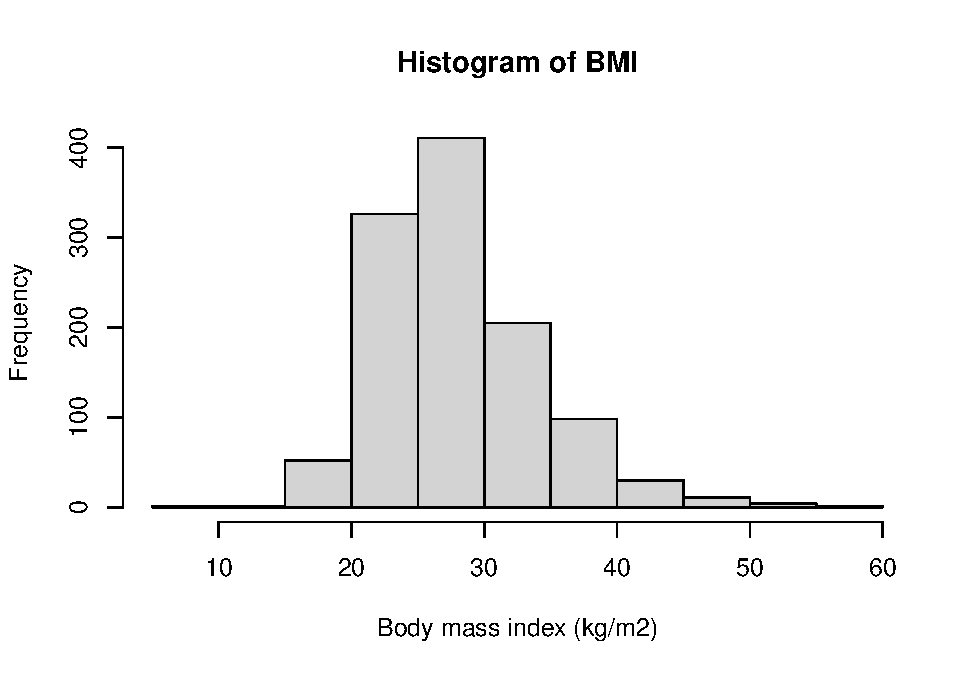
\includegraphics{phcm9795-solutions-R_files/figure-latex/unnamed-chunk-24-1.pdf}

\begin{Shaded}
\begin{Highlighting}[]
\FunctionTok{boxplot}\NormalTok{(survey}\SpecialCharTok{$}\NormalTok{bmi, }\AttributeTok{main=}\StringTok{"Boxplot of BMI"}\NormalTok{, }\AttributeTok{ylab=}\StringTok{"Body mass index (kg/m2)"}\NormalTok{)}
\end{Highlighting}
\end{Shaded}

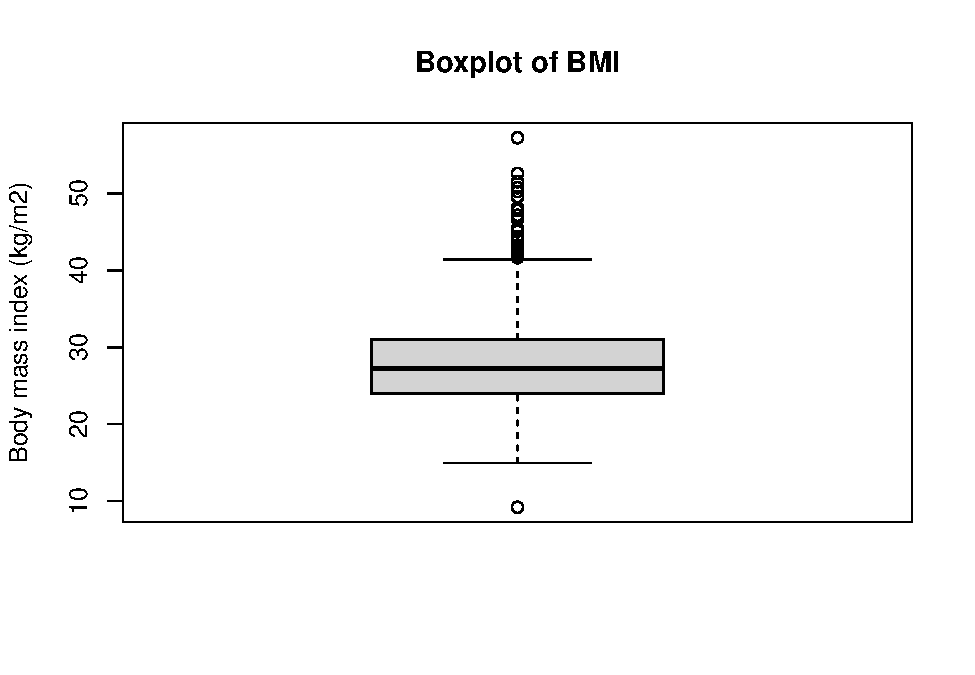
\includegraphics{phcm9795-solutions-R_files/figure-latex/unnamed-chunk-24-2.pdf}

\begin{quote}
The boxplot in particular shows that there are some extreme values of BMI. We can examine these records by viewing records with BMI less than, say 15, or greater than 45:
\end{quote}

\begin{Shaded}
\begin{Highlighting}[]
\FunctionTok{subset}\NormalTok{(survey, bmi}\SpecialCharTok{\textless{}}\DecValTok{15}\NormalTok{)}
\end{Highlighting}
\end{Shaded}

\begin{verbatim}
## # A tibble: 2 x 4
##   sex    height weight   bmi
##   <fct>   <dbl>  <dbl> <dbl>
## 1 Female   1.57   22.7  9.21
## 2 Female   1.65   40.8 15.0
\end{verbatim}

\begin{Shaded}
\begin{Highlighting}[]
\FunctionTok{subset}\NormalTok{(survey, bmi}\SpecialCharTok{\textgreater{}}\DecValTok{45}\NormalTok{)}
\end{Highlighting}
\end{Shaded}

\begin{verbatim}
## # A tibble: 16 x 4
##    sex    height weight   bmi
##    <fct>   <dbl>  <dbl> <dbl>
##  1 Female   1.52  105    45.4
##  2 Male     1.85  174.   50.8
##  3 Female   1.22   74.8  50.3
##  4 Male     1.93  213.   57.2
##  5 Female   1.63  127    47.8
##  6 Female   1.55  115.   48.0
##  7 Female   1.65  131.   48.2
##  8 Female   1.55  109.   45.3
##  9 Male     1.78  143.   45.1
## 10 Female   1.65  127    46.6
## 11 Female   1.63  132.   49.5
## 12 Female   1.7   152    52.6
## 13 Female   1.6   127    49.6
## 14 Female   1.5   106.   47.2
## 15 Female   1.73  154.   51.5
## 16 Female   1.6   116.   45.4
\end{verbatim}

\begin{quote}
The smallest BMI of 9.2 kg/m2 is very low, with a weight of 22.7 kg. We should check the recorded height and weight values against the original data (paper records, survey responses) if they were available. However, as a weight of 22.7kg is not impossible, this record will not be deleted. An alternative approach would be to analyse the data including the very low BMI and again excluding the very low BMI as a sensitivity analysis.
The largest BMI values are based on participants with large weights, and none of these seem biologically implausible. Therefore, no changes will be made to participants with small or large values of BMI.
\end{quote}

\begin{quote}
We can use the \texttt{cut()} function to create the BMI categories. The WHO cutpoints are inclusive of the lower-bound, so we use \texttt{right=FALSE}. After creating the categories, it is good practice to check the resulting categories using \texttt{summary()}:
\end{quote}

\begin{Shaded}
\begin{Highlighting}[]
\NormalTok{survey}\SpecialCharTok{$}\NormalTok{bmi\_cat }\OtherTok{\textless{}{-}} \FunctionTok{cut}\NormalTok{(survey}\SpecialCharTok{$}\NormalTok{bmi, }\FunctionTok{c}\NormalTok{(}\DecValTok{0}\NormalTok{, }\FloatTok{18.5}\NormalTok{, }\DecValTok{25}\NormalTok{, }\DecValTok{30}\NormalTok{, }\DecValTok{35}\NormalTok{, }\DecValTok{40}\NormalTok{, }\DecValTok{100}\NormalTok{), }\AttributeTok{right=}\ConstantTok{FALSE}\NormalTok{)}
\FunctionTok{summary}\NormalTok{(survey}\SpecialCharTok{$}\NormalTok{bmi\_cat)}
\end{Highlighting}
\end{Shaded}

\begin{verbatim}
##  [0,18.5) [18.5,25)   [25,30)   [30,35)   [35,40)  [40,100) 
##        18       362       411       201       101        47
\end{verbatim}

\begin{quote}
Finally, we can create a two-way table using the \texttt{contTables()} function within the \texttt{jmv} package. We can define the rows by BMI category, and the columns by sex:
\end{quote}

\begin{Shaded}
\begin{Highlighting}[]
\FunctionTok{contTables}\NormalTok{(}\AttributeTok{data=}\NormalTok{survey,}
           \AttributeTok{rows =}\NormalTok{ bmi\_cat,}
           \AttributeTok{cols =}\NormalTok{ sex)}
\end{Highlighting}
\end{Shaded}

\begin{verbatim}
## 
##  CONTINGENCY TABLES
## 
##  Contingency Tables                       
##  ──────────────────────────────────────── 
##    bmi_cat      Male    Female    Total   
##  ──────────────────────────────────────── 
##    [0,18.5)        6        12       18   
##    [18.5,25)     134       228      362   
##    [25,30)       216       195      411   
##    [30,35)        95       106      201   
##    [35,40)        46        55      101   
##    [40,100)       16        31       47   
##    Total         513       627     1140   
##  ──────────────────────────────────────── 
## 
## 
##  χ² Tests                              
##  ───────────────────────────────────── 
##          Value       df    p           
##  ───────────────────────────────────── 
##    χ²    22.49802     5    0.0004209   
##    N         1140                      
##  ─────────────────────────────────────
\end{verbatim}

\begin{quote}
To assess whether there is a difference in BMI between males and females, we should look at the within-sex relative frequencies. In other words, column percents (for this table), by specifying \texttt{pcCol\ =\ TRUE}:
\end{quote}

\begin{Shaded}
\begin{Highlighting}[]
\FunctionTok{contTables}\NormalTok{(}\AttributeTok{data=}\NormalTok{survey,}
           \AttributeTok{rows =}\NormalTok{ bmi\_cat,}
           \AttributeTok{cols =}\NormalTok{ sex,}
           \AttributeTok{pcCol =} \ConstantTok{TRUE}\NormalTok{)}
\end{Highlighting}
\end{Shaded}

\begin{verbatim}
## 
##  CONTINGENCY TABLES
## 
##  Contingency Tables                                                      
##  ─────────────────────────────────────────────────────────────────────── 
##    bmi_cat                         Male         Female       Total       
##  ─────────────────────────────────────────────────────────────────────── 
##    [0,18.5)     Observed                   6           12           18   
##                 % within column      1.16959      1.91388      1.57895   
##                                                                          
##    [18.5,25)    Observed                 134          228          362   
##                 % within column     26.12086     36.36364     31.75439   
##                                                                          
##    [25,30)      Observed                 216          195          411   
##                 % within column     42.10526     31.10048     36.05263   
##                                                                          
##    [30,35)      Observed                  95          106          201   
##                 % within column     18.51852     16.90590     17.63158   
##                                                                          
##    [35,40)      Observed                  46           55          101   
##                 % within column      8.96686      8.77193      8.85965   
##                                                                          
##    [40,100)     Observed                  16           31           47   
##                 % within column      3.11891      4.94418      4.12281   
##                                                                          
##    Total        Observed                 513          627         1140   
##                 % within column    100.00000    100.00000    100.00000   
##  ─────────────────────────────────────────────────────────────────────── 
## 
## 
##  χ² Tests                              
##  ───────────────────────────────────── 
##          Value       df    p           
##  ───────────────────────────────────── 
##    χ²    22.49802     5    0.0004209   
##    N         1140                      
##  ─────────────────────────────────────
\end{verbatim}

\begin{quote}
From this health survey, it appears that men are more likely to have BMIs indicating Pre-Obesity (men 42\% vs women 31\%) and Obesity Class I (men 19\% vs women 17\%), compared to women who are more likely to have BMIs indicating Normal weight (women 36\% vs men 26\%).
\end{quote}

\hypertarget{activity-2.5}{%
\subsection*{Activity 2.5}\label{activity-2.5}}
\addcontentsline{toc}{subsection}{Activity 2.5}

The data in the file \texttt{Activity\_S2.5.rds} (available on Moodle) has information about birth weight and length of stay collected from 117 babies admitted consecutively to a hospital for surgery. For each variable:

\begin{enumerate}
\def\labelenumi{\alph{enumi}.}
\tightlist
\item
  Create a histogram to inspect the distribution of the variable;
\end{enumerate}

\begin{Shaded}
\begin{Highlighting}[]
\NormalTok{babies }\OtherTok{\textless{}{-}} \FunctionTok{readRDS}\NormalTok{(}\StringTok{"data/activities/Activity\_S2.5{-}LengthOfStay.rds"}\NormalTok{)}
\FunctionTok{summary}\NormalTok{(babies)}
\end{Highlighting}
\end{Shaded}

\begin{verbatim}
##        ID          Sex        BirthWt        GestAge        LengthStay    
##  Min.   : 25   female:55   Min.   :1500   Min.   :31.00   Min.   :  0.00  
##  1st Qu.: 54   male  :62   1st Qu.:2012   1st Qu.:35.75   1st Qu.: 21.00  
##  Median : 83               Median :2438   Median :36.00   Median : 30.00  
##  Mean   : 83               Mean   :2451   Mean   :36.56   Mean   : 41.08  
##  3rd Qu.:112               3rd Qu.:2830   3rd Qu.:38.00   3rd Qu.: 43.00  
##  Max.   :141               Max.   :3545   Max.   :41.00   Max.   :244.00  
##                            NA's   :1      NA's   :5
\end{verbatim}

\begin{Shaded}
\begin{Highlighting}[]
\FunctionTok{hist}\NormalTok{(babies}\SpecialCharTok{$}\NormalTok{BirthWt, }\AttributeTok{main=}\StringTok{"Histogram of birth weights"}\NormalTok{,}
     \AttributeTok{xlab=}\StringTok{"Birth weight (kg)"}\NormalTok{)}
\end{Highlighting}
\end{Shaded}

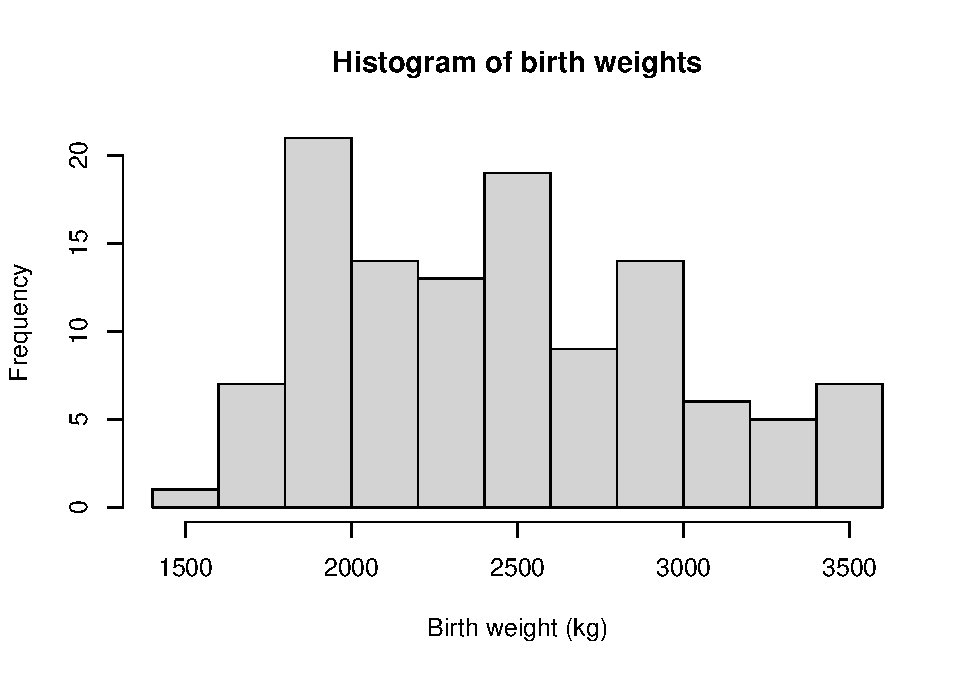
\includegraphics{phcm9795-solutions-R_files/figure-latex/unnamed-chunk-29-1.pdf}

\begin{Shaded}
\begin{Highlighting}[]
\CommentTok{\# We can specify our own cutpoints using the breaks command, with the seq() function:}
\FunctionTok{hist}\NormalTok{(babies}\SpecialCharTok{$}\NormalTok{BirthWt, }\AttributeTok{main=}\StringTok{"Histogram of birth weights"}\NormalTok{,}
     \AttributeTok{xlab=}\StringTok{"Birth weight (kg)"}\NormalTok{,}
     \AttributeTok{breaks=}\FunctionTok{seq}\NormalTok{(}\AttributeTok{from=}\DecValTok{1500}\NormalTok{, }\AttributeTok{to=}\DecValTok{4000}\NormalTok{, }\AttributeTok{by=}\DecValTok{250}\NormalTok{))}
\end{Highlighting}
\end{Shaded}

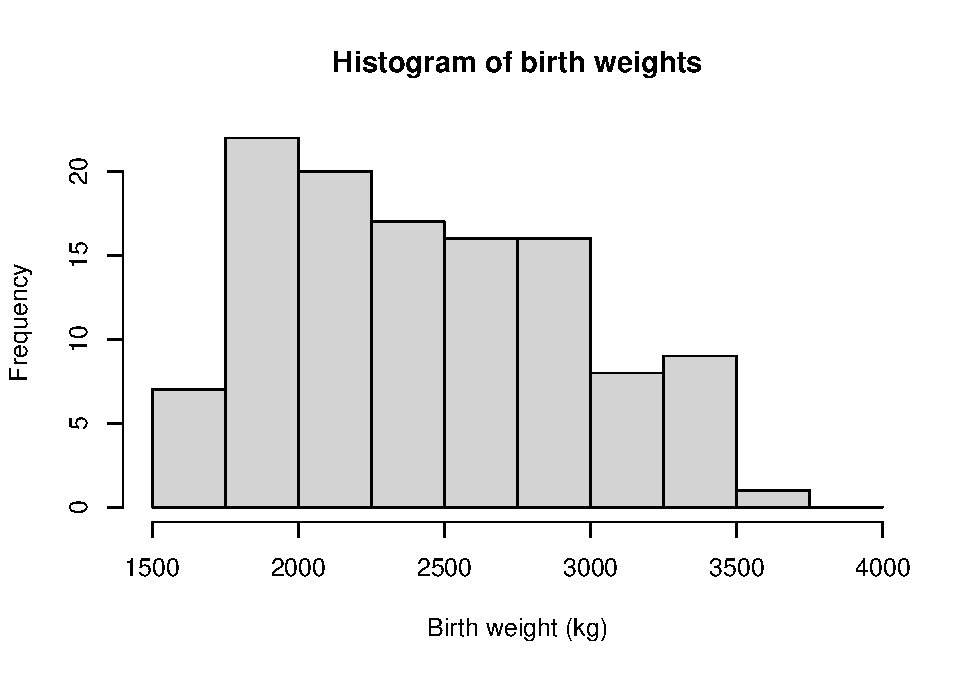
\includegraphics{phcm9795-solutions-R_files/figure-latex/unnamed-chunk-29-2.pdf}

\begin{Shaded}
\begin{Highlighting}[]
\FunctionTok{hist}\NormalTok{(babies}\SpecialCharTok{$}\NormalTok{LengthStay, }\AttributeTok{main=}\StringTok{"Histogram of lengths of stay"}\NormalTok{,}
     \AttributeTok{xlab=}\StringTok{"Length of stay (days)"}\NormalTok{)}
\end{Highlighting}
\end{Shaded}

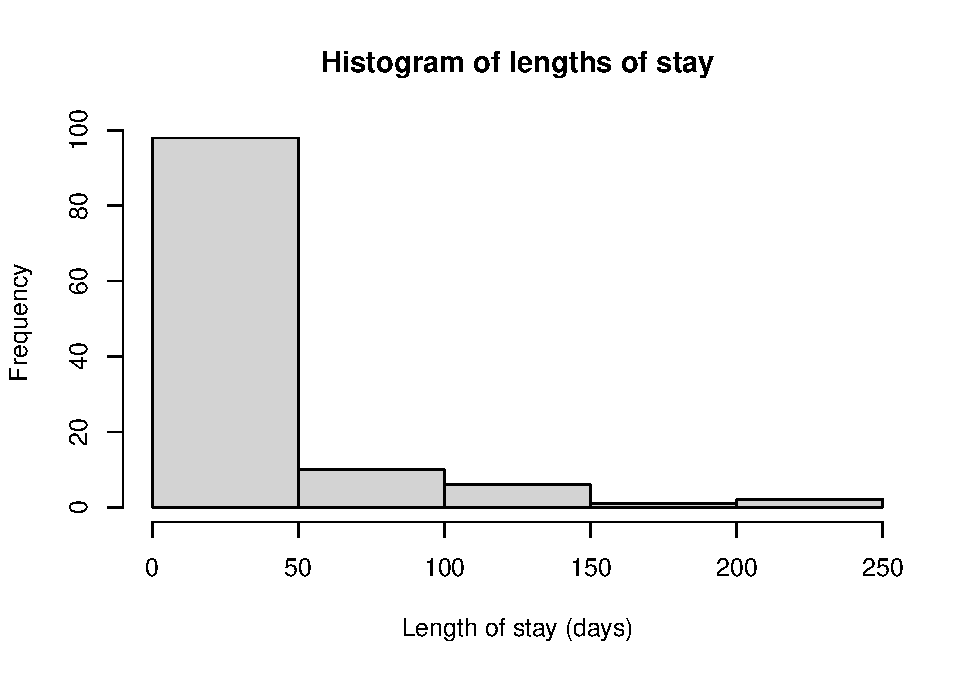
\includegraphics{phcm9795-solutions-R_files/figure-latex/unnamed-chunk-29-3.pdf}

\begin{Shaded}
\begin{Highlighting}[]
\FunctionTok{hist}\NormalTok{(babies}\SpecialCharTok{$}\NormalTok{LengthStay, }\AttributeTok{main=}\StringTok{"Histogram of lengths of stay"}\NormalTok{,}
     \AttributeTok{xlab=}\StringTok{"Length of stay (days)"}\NormalTok{,}
     \AttributeTok{breaks=}\FunctionTok{seq}\NormalTok{(}\AttributeTok{from=}\DecValTok{0}\NormalTok{, }\AttributeTok{to=}\DecValTok{250}\NormalTok{, }\AttributeTok{by=}\DecValTok{25}\NormalTok{))}
\end{Highlighting}
\end{Shaded}

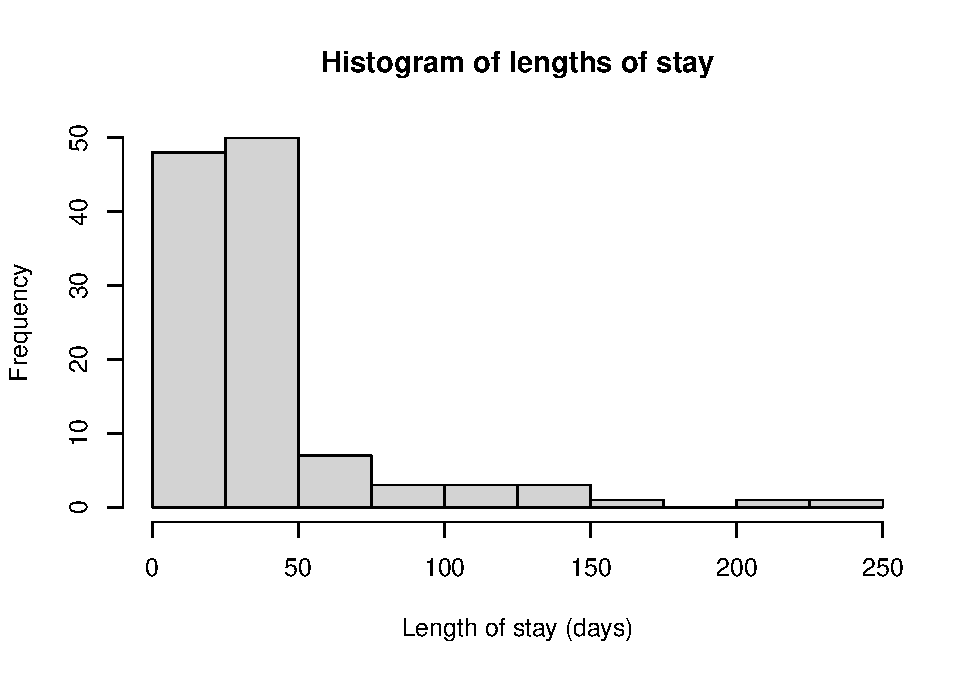
\includegraphics{phcm9795-solutions-R_files/figure-latex/unnamed-chunk-29-4.pdf}

\begin{quote}
The histogram for birthweight shows a roughly symmetric distribution. The histogram for length of stay shows a highly skewed distribution (skewed to the right).
\end{quote}

\begin{enumerate}
\def\labelenumi{\alph{enumi}.}
\setcounter{enumi}{1}
\tightlist
\item
  Complete the following summary statistics for each variable:

  \begin{itemize}
  \tightlist
  \item
    mean and median;
  \item
    standard deviation and interquartile range;
  \item
    skewness and kurtosis.
  \end{itemize}
\end{enumerate}

\begin{Shaded}
\begin{Highlighting}[]
\FunctionTok{descriptives}\NormalTok{(}\AttributeTok{data =}\NormalTok{ babies,}
             \AttributeTok{vars =} \FunctionTok{c}\NormalTok{(BirthWt, LengthStay),}
             \AttributeTok{pc =} \ConstantTok{TRUE}\NormalTok{,}
             \AttributeTok{skew =} \ConstantTok{TRUE}\NormalTok{,}
             \AttributeTok{kurt =} \ConstantTok{TRUE}\NormalTok{)}
\end{Highlighting}
\end{Shaded}

\begin{verbatim}
## 
##  DESCRIPTIVES
## 
##  Descriptives                                        
##  ─────────────────────────────────────────────────── 
##                           BirthWt       LengthStay   
##  ─────────────────────────────────────────────────── 
##    N                             116           117   
##    Missing                         1             0   
##    Mean                     2451.207      41.07692   
##    Median                   2437.500      30.00000   
##    Standard deviation       504.8221      36.92984   
##    Minimum                  1500.000      0.000000   
##    Maximum                  3545.000      244.0000   
##    Skewness                0.3548827      3.090351   
##    Std. error skewness     0.2245612     0.2236233   
##    Kurtosis               -0.7448547      11.56803   
##    Std. error kurtosis     0.4455276     0.4436951   
##    25th percentile          2012.000      21.00000   
##    50th percentile          2437.500      30.00000   
##    75th percentile          2830.000      43.00000   
##  ───────────────────────────────────────────────────
\end{verbatim}

Make a decision about whether each variable is symmetric or not, and which measure of central tendency and variability should be reported.

\begin{quote}
As birthweight follows a roughly symmetric distribution, we should present the mean and standard deviation as the appropriate measures of central tendency and spread. Notice that the mean and median are similar, which is to be expected for a symmetric distribution.
\end{quote}

\begin{quote}
Length of stay is highly skewed. In this case, the median and interquartile range are the appropriate measures to present. Notice that the mean is higher than the median, which is typical for distributions that are skewed to the right.
\end{quote}

\hypertarget{activity-2.6}{%
\subsection*{Activity 2.6}\label{activity-2.6}}
\addcontentsline{toc}{subsection}{Activity 2.6}

The data set of hospital stay data for 1323 hypothetical patients is available on Moodle in csv format (\texttt{Activity2.6.csv}). Import this dataset into R There are two variables in this dataset:

\begin{itemize}
\tightlist
\item
  female: female=1; male=0
\item
  los: length of stay in days
\end{itemize}

\begin{enumerate}
\def\labelenumi{\alph{enumi})}
\tightlist
\item
  Use R to examine the distribution of length of stay: overall; and separately for females and males. Comment on the distributions.
\end{enumerate}

\begin{Shaded}
\begin{Highlighting}[]
\NormalTok{hospstay }\OtherTok{\textless{}{-}} \FunctionTok{read.csv}\NormalTok{(}\StringTok{"data/activities/Activity\_S2.5.csv"}\NormalTok{)}

\FunctionTok{summary}\NormalTok{(hospstay)}
\end{Highlighting}
\end{Shaded}

\begin{verbatim}
##      female            los        
##  Min.   :0.0000   Min.   :  0.00  
##  1st Qu.:0.0000   1st Qu.:  4.00  
##  Median :0.0000   Median :  9.00  
##  Mean   :0.1104   Mean   : 12.52  
##  3rd Qu.:0.0000   3rd Qu.: 17.00  
##  Max.   :1.0000   Max.   :106.00
\end{verbatim}

\begin{Shaded}
\begin{Highlighting}[]
\CommentTok{\# Define female as a factor}
\NormalTok{hospstay}\SpecialCharTok{$}\NormalTok{female }\OtherTok{\textless{}{-}} \FunctionTok{factor}\NormalTok{(hospstay}\SpecialCharTok{$}\NormalTok{female, }\AttributeTok{levels=}\FunctionTok{c}\NormalTok{(}\DecValTok{0}\NormalTok{,}\DecValTok{1}\NormalTok{), }\AttributeTok{labels=}\FunctionTok{c}\NormalTok{(}\StringTok{"Male"}\NormalTok{, }\StringTok{"Female"}\NormalTok{))}
\FunctionTok{summary}\NormalTok{(hospstay}\SpecialCharTok{$}\NormalTok{female)}
\end{Highlighting}
\end{Shaded}

\begin{verbatim}
##   Male Female 
##   1177    146
\end{verbatim}

\begin{Shaded}
\begin{Highlighting}[]
\FunctionTok{hist}\NormalTok{(hospstay}\SpecialCharTok{$}\NormalTok{los, }\AttributeTok{main=}\StringTok{"Histogram of hospital stay"}\NormalTok{, }\AttributeTok{xlab=}\StringTok{"Length of stay (days)"}\NormalTok{)}
\end{Highlighting}
\end{Shaded}

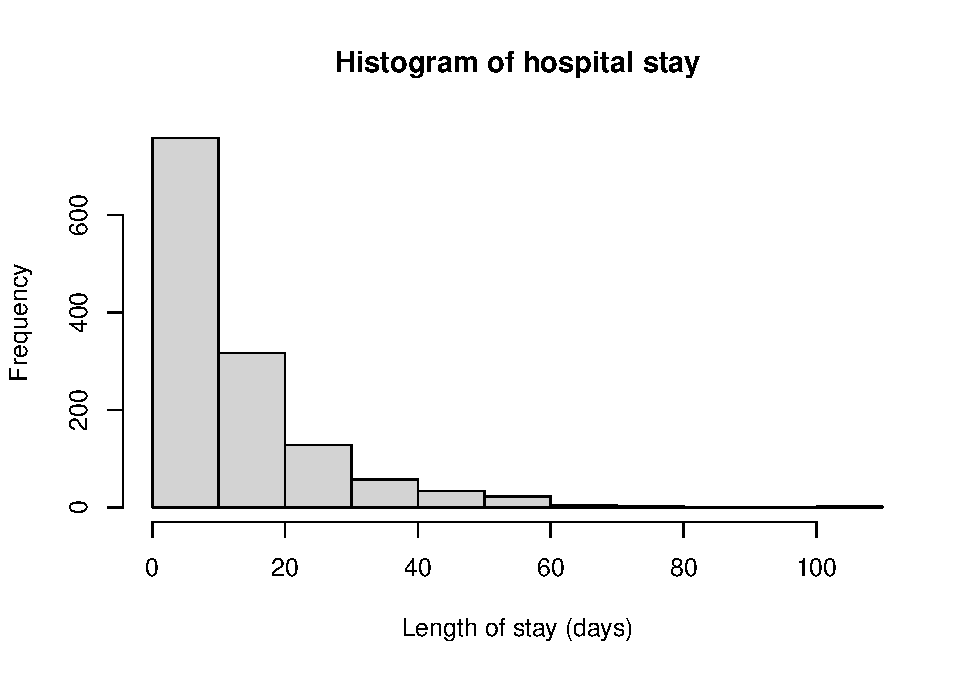
\includegraphics{phcm9795-solutions-R_files/figure-latex/unnamed-chunk-31-1.pdf}

\begin{Shaded}
\begin{Highlighting}[]
\FunctionTok{boxplot}\NormalTok{(hospstay}\SpecialCharTok{$}\NormalTok{los, }\AttributeTok{main=}\StringTok{"Boxplot of hospital stay"}\NormalTok{, }\AttributeTok{ylab=}\StringTok{"Length of stay (days)"}\NormalTok{)}
\end{Highlighting}
\end{Shaded}

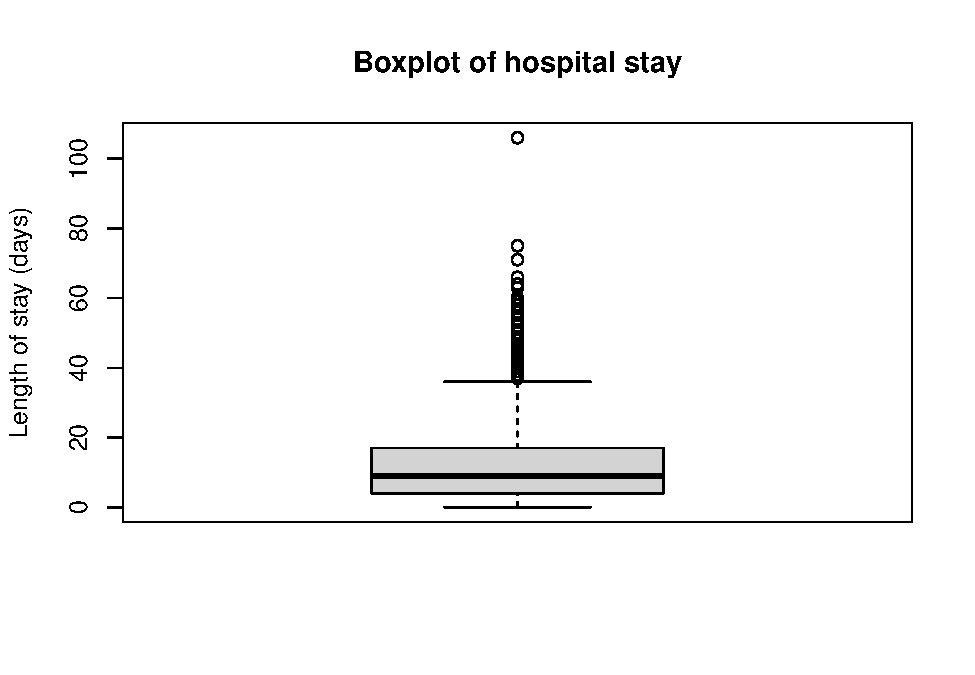
\includegraphics{phcm9795-solutions-R_files/figure-latex/unnamed-chunk-31-2.pdf}

\begin{Shaded}
\begin{Highlighting}[]
\NormalTok{hospstay\_males }\OtherTok{\textless{}{-}} \FunctionTok{subset}\NormalTok{(hospstay, female}\SpecialCharTok{==}\StringTok{"Male"}\NormalTok{)}
\NormalTok{hospstay\_females }\OtherTok{\textless{}{-}} \FunctionTok{subset}\NormalTok{(hospstay, female}\SpecialCharTok{==}\StringTok{"Female"}\NormalTok{)}

\CommentTok{\# Set the graphics parameters to plot 2 rows and 2 columns:}
\FunctionTok{par}\NormalTok{(}\AttributeTok{mfrow=}\FunctionTok{c}\NormalTok{(}\DecValTok{2}\NormalTok{,}\DecValTok{2}\NormalTok{))}

\CommentTok{\# Specify each plot separately}
\FunctionTok{hist}\NormalTok{(hospstay\_males}\SpecialCharTok{$}\NormalTok{los, }\AttributeTok{xlab=}\StringTok{"Length of stay (days)"}\NormalTok{, }\AttributeTok{main=}\StringTok{"Males"}\NormalTok{)}
\FunctionTok{hist}\NormalTok{(hospstay\_females}\SpecialCharTok{$}\NormalTok{los, }\AttributeTok{xlab=}\StringTok{"Length of stay (days)"}\NormalTok{, }\AttributeTok{main=}\StringTok{"Females"}\NormalTok{)}

\FunctionTok{boxplot}\NormalTok{(hospstay\_males}\SpecialCharTok{$}\NormalTok{los, }\AttributeTok{ylab=}\StringTok{"Length of stay (days)"}\NormalTok{, }\AttributeTok{main=}\StringTok{"Males"}\NormalTok{)}
\FunctionTok{boxplot}\NormalTok{(hospstay\_females}\SpecialCharTok{$}\NormalTok{los, }\AttributeTok{ylab=}\StringTok{"Length of stay (days)"}\NormalTok{, }\AttributeTok{main=}\StringTok{"Females"}\NormalTok{)}
\end{Highlighting}
\end{Shaded}

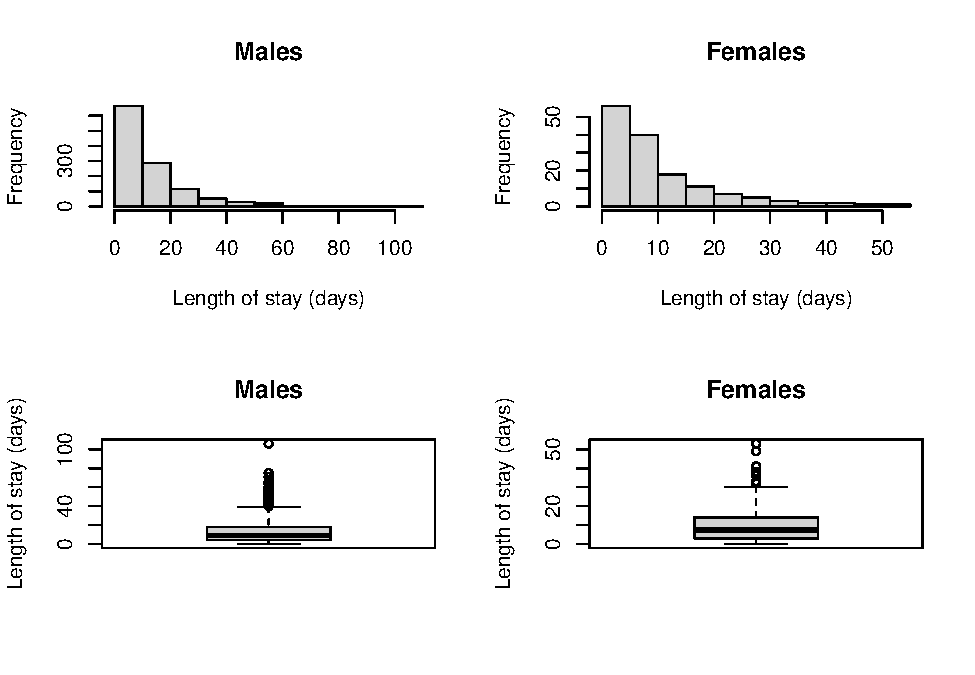
\includegraphics{phcm9795-solutions-R_files/figure-latex/unnamed-chunk-31-3.pdf}

\begin{Shaded}
\begin{Highlighting}[]
\CommentTok{\# Reset graphics parameters}
\FunctionTok{par}\NormalTok{(}\AttributeTok{mfrow=}\FunctionTok{c}\NormalTok{(}\DecValTok{1}\NormalTok{,}\DecValTok{1}\NormalTok{))}
\end{Highlighting}
\end{Shaded}

\begin{quote}
The histograms for overall length of stay and length of stay by gender all show that length of stay is heavily skewed (skewed to the right).
\end{quote}

\begin{enumerate}
\def\labelenumi{\alph{enumi})}
\setcounter{enumi}{1}
\tightlist
\item
  Use R to calculate measures of central tendency for hospital stay to obtain information about the average duration of hospital stay. Which summary statistics should you report and why? Report the appropriate statistics of the spread and measure of central tendency chosen.
\end{enumerate}

\begin{Shaded}
\begin{Highlighting}[]
\FunctionTok{descriptives}\NormalTok{(}\AttributeTok{data =}\NormalTok{ hospstay,}
             \AttributeTok{vars =}\NormalTok{ los,}
             \AttributeTok{pc =} \ConstantTok{TRUE}\NormalTok{,}
             \AttributeTok{skew =} \ConstantTok{TRUE}\NormalTok{,}
             \AttributeTok{kurt =} \ConstantTok{TRUE}\NormalTok{)}
\end{Highlighting}
\end{Shaded}

\begin{verbatim}
## 
##  DESCRIPTIVES
## 
##  Descriptives                          
##  ───────────────────────────────────── 
##                           los          
##  ───────────────────────────────────── 
##    N                            1323   
##    Missing                         0   
##    Mean                     12.51550   
##    Median                          9   
##    Standard deviation       12.59933   
##    Minimum                         0   
##    Maximum                       106   
##    Skewness                 1.947803   
##    Std. error skewness    0.06726732   
##    Kurtosis                 5.166837   
##    Std. error kurtosis     0.1344336   
##    25th percentile          4.000000   
##    50th percentile          9.000000   
##    75th percentile          17.00000   
##  ─────────────────────────────────────
\end{verbatim}

\begin{quote}
As the distribution of length of stay is highly skewed, the median and interquartile range should be presented. These can be calculated in the usual way, using the \texttt{descriptives()} function. The median length of stay is 9 days, with an interquartile range of 4 to 17 days.
\end{quote}

\begin{enumerate}
\def\labelenumi{\alph{enumi})}
\setcounter{enumi}{2}
\tightlist
\item
  Calculate the measures of central tendency for hospital duration separately for males and females. What can you conclude from comparing these measures for males and females?
\end{enumerate}

\begin{Shaded}
\begin{Highlighting}[]
\FunctionTok{descriptives}\NormalTok{(}\AttributeTok{data =}\NormalTok{ hospstay,}
             \AttributeTok{vars =}\NormalTok{ los,}
             \AttributeTok{splitBy =}\NormalTok{ female,}
             \AttributeTok{pc =} \ConstantTok{TRUE}\NormalTok{,}
             \AttributeTok{skew =} \ConstantTok{TRUE}\NormalTok{,}
             \AttributeTok{kurt =} \ConstantTok{TRUE}\NormalTok{)}
\end{Highlighting}
\end{Shaded}

\begin{verbatim}
## 
##  DESCRIPTIVES
## 
##  Descriptives                                    
##  ─────────────────────────────────────────────── 
##                           female    los          
##  ─────────────────────────────────────────────── 
##    N                      Male            1177   
##                           Female           146   
##    Missing                Male               0   
##                           Female             0   
##    Mean                   Male        12.75531   
##                           Female      10.58219   
##    Median                 Male               9   
##                           Female      7.500000   
##    Standard deviation     Male        12.83475   
##                           Female      10.34625   
##    Minimum                Male               0   
##                           Female             0   
##    Maximum                Male             106   
##                           Female            53   
##    Skewness               Male        1.943967   
##                           Female      1.697009   
##    Std. error skewness    Male      0.07130745   
##                           Female     0.2006795   
##    Kurtosis               Male        5.128450   
##                           Female      3.067601   
##    Std. error kurtosis    Male       0.1424946   
##                           Female     0.3987670   
##    25th percentile        Male        4.000000   
##                           Female      3.000000   
##    50th percentile        Male        9.000000   
##                           Female      7.500000   
##    75th percentile        Male        18.00000   
##                           Female      14.00000   
##  ───────────────────────────────────────────────
\end{verbatim}

\begin{quote}
Lengths of stay are similar for men (median: 9 days, interquartile range: 4 to 18 days) and women (median: 8 days, interquartile range: 3 to 14 days).
\end{quote}

\hypertarget{module-2-full-script}{%
\chapter*{Module 2: Full script}\label{module-2-full-script}}
\addcontentsline{toc}{chapter}{Module 2: Full script}

\begin{Shaded}
\begin{Highlighting}[]
\CommentTok{\# Author: Timothy Dobbins}
\CommentTok{\# Date: May, 2022}
\CommentTok{\# Purpose: Learning activities for Module 2}

\FunctionTok{library}\NormalTok{(jmv)}
\FunctionTok{library}\NormalTok{(readxl)}

\DocumentationTok{\#\#\# Activity 2.1}

\FunctionTok{pbinom}\NormalTok{(}\AttributeTok{q=}\DecValTok{59}\NormalTok{, }\AttributeTok{size=}\DecValTok{90}\NormalTok{, }\AttributeTok{prob=}\FloatTok{0.5}\NormalTok{, }\AttributeTok{lower.tail =} \ConstantTok{FALSE}\NormalTok{)}


\DocumentationTok{\#\#\# Activity 2.2}

\FunctionTok{dbinom}\NormalTok{(}\AttributeTok{x=}\DecValTok{0}\NormalTok{, }\AttributeTok{size=}\DecValTok{5}\NormalTok{, }\AttributeTok{prob=}\FloatTok{0.35}\NormalTok{)}
\FunctionTok{dbinom}\NormalTok{(}\AttributeTok{x=}\DecValTok{2}\NormalTok{, }\AttributeTok{size=}\DecValTok{5}\NormalTok{, }\AttributeTok{prob=}\FloatTok{0.35}\NormalTok{)}
\FunctionTok{dbinom}\NormalTok{(}\AttributeTok{x=}\DecValTok{5}\NormalTok{, }\AttributeTok{size=}\DecValTok{5}\NormalTok{, }\AttributeTok{prob=}\FloatTok{0.35}\NormalTok{)}
\FunctionTok{pbinom}\NormalTok{(}\AttributeTok{q=}\DecValTok{3}\NormalTok{, }\AttributeTok{size=}\DecValTok{5}\NormalTok{, }\AttributeTok{prob=}\FloatTok{0.35}\NormalTok{)}


\DocumentationTok{\#\#\# Activity 2.3}
\NormalTok{A }\OtherTok{\textless{}{-}} \FunctionTok{pnorm}\NormalTok{(}\DecValTok{75}\NormalTok{, }\AttributeTok{mean=}\DecValTok{87}\NormalTok{, }\AttributeTok{sd=}\DecValTok{8}\NormalTok{, }\AttributeTok{lower.tail=}\ConstantTok{TRUE}\NormalTok{)}
\NormalTok{A}

\NormalTok{C }\OtherTok{\textless{}{-}} \FunctionTok{pnorm}\NormalTok{(}\DecValTok{95}\NormalTok{, }\AttributeTok{mean=}\DecValTok{87}\NormalTok{, }\AttributeTok{sd=}\DecValTok{8}\NormalTok{, }\AttributeTok{lower.tail=}\ConstantTok{FALSE}\NormalTok{)   }
\NormalTok{C}

\NormalTok{B }\OtherTok{\textless{}{-}} \DecValTok{1} \SpecialCharTok{{-}}\NormalTok{ A }\SpecialCharTok{{-}}\NormalTok{ C}
\NormalTok{B}


\DocumentationTok{\#\#\# Activity 2.4}

\NormalTok{survey }\OtherTok{\textless{}{-}} \FunctionTok{read\_excel}\NormalTok{(}\StringTok{"data/examples/health{-}survey.xlsx"}\NormalTok{)}
\FunctionTok{summary}\NormalTok{(survey)}

\NormalTok{survey}\SpecialCharTok{$}\NormalTok{sex }\OtherTok{\textless{}{-}} \FunctionTok{factor}\NormalTok{(survey}\SpecialCharTok{$}\NormalTok{sex, }\AttributeTok{level=}\FunctionTok{c}\NormalTok{(}\DecValTok{1}\NormalTok{,}\DecValTok{2}\NormalTok{), }\AttributeTok{labels=}\FunctionTok{c}\NormalTok{(}\StringTok{"Male"}\NormalTok{, }\StringTok{"Female"}\NormalTok{))}

\NormalTok{survey}\SpecialCharTok{$}\NormalTok{bmi }\OtherTok{=}\NormalTok{ survey}\SpecialCharTok{$}\NormalTok{weight }\SpecialCharTok{/}\NormalTok{ (survey}\SpecialCharTok{$}\NormalTok{height}\SpecialCharTok{\^{}}\DecValTok{2}\NormalTok{)}
\FunctionTok{hist}\NormalTok{(survey}\SpecialCharTok{$}\NormalTok{bmi, }\AttributeTok{main=}\StringTok{"Histogram of BMI"}\NormalTok{, }\AttributeTok{xlab=}\StringTok{"BMI (kg/m2)"}\NormalTok{)}
\FunctionTok{boxplot}\NormalTok{(survey}\SpecialCharTok{$}\NormalTok{bmi, }\AttributeTok{main=}\StringTok{"Boxplot of BMI"}\NormalTok{, }\AttributeTok{ylab=}\StringTok{"BMI (kg/m2)"}\NormalTok{)}

\FunctionTok{subset}\NormalTok{(survey, bmi}\SpecialCharTok{\textless{}}\DecValTok{15}\NormalTok{)}
\FunctionTok{subset}\NormalTok{(survey, bmi}\SpecialCharTok{\textgreater{}}\DecValTok{45}\NormalTok{)}

\NormalTok{survey}\SpecialCharTok{$}\NormalTok{bmi\_cat }\OtherTok{\textless{}{-}} \FunctionTok{cut}\NormalTok{(survey}\SpecialCharTok{$}\NormalTok{bmi, }\FunctionTok{c}\NormalTok{(}\DecValTok{0}\NormalTok{, }\FloatTok{18.5}\NormalTok{, }\DecValTok{25}\NormalTok{, }\DecValTok{30}\NormalTok{, }\DecValTok{35}\NormalTok{, }\DecValTok{40}\NormalTok{, }\DecValTok{100}\NormalTok{), }\AttributeTok{right=}\ConstantTok{FALSE}\NormalTok{)}
\FunctionTok{summary}\NormalTok{(survey}\SpecialCharTok{$}\NormalTok{bmi\_cat)}

\FunctionTok{contTables}\NormalTok{(}\AttributeTok{data=}\NormalTok{survey,}
           \AttributeTok{rows =}\NormalTok{ bmi\_cat,}
           \AttributeTok{cols =}\NormalTok{ sex)}

\FunctionTok{contTables}\NormalTok{(}\AttributeTok{data=}\NormalTok{survey,}
           \AttributeTok{rows =}\NormalTok{ bmi\_cat,}
           \AttributeTok{cols =}\NormalTok{ sex,}
           \AttributeTok{pcCol =} \ConstantTok{TRUE}\NormalTok{)}

\DocumentationTok{\#\#\# Activity 2.5}
\NormalTok{babies }\OtherTok{\textless{}{-}} \FunctionTok{readRDS}\NormalTok{(}\StringTok{"data/activities/Activity\_S2.5{-}LengthOfStay.rds"}\NormalTok{)}
\FunctionTok{summary}\NormalTok{(babies)}

\FunctionTok{hist}\NormalTok{(babies}\SpecialCharTok{$}\NormalTok{BirthWt, }\AttributeTok{main=}\StringTok{"Histogram of birth weights"}\NormalTok{,}
     \AttributeTok{xlab=}\StringTok{"Birth weight (kg)"}\NormalTok{)}

\CommentTok{\# We can specify our own cutpoints using the breaks command, with the seq() function:}
\FunctionTok{hist}\NormalTok{(babies}\SpecialCharTok{$}\NormalTok{BirthWt, }\AttributeTok{main=}\StringTok{"Histogram of birth weights"}\NormalTok{,}
     \AttributeTok{xlab=}\StringTok{"Birth weight (kg)"}\NormalTok{,}
     \AttributeTok{breaks=}\FunctionTok{seq}\NormalTok{(}\AttributeTok{from=}\DecValTok{1500}\NormalTok{, }\AttributeTok{to=}\DecValTok{4000}\NormalTok{, }\AttributeTok{by=}\DecValTok{250}\NormalTok{))}

\FunctionTok{hist}\NormalTok{(babies}\SpecialCharTok{$}\NormalTok{LengthStay, }\AttributeTok{main=}\StringTok{"Histogram of lengths of stay"}\NormalTok{,}
     \AttributeTok{xlab=}\StringTok{"Length of stay (days)"}\NormalTok{)}

\FunctionTok{hist}\NormalTok{(babies}\SpecialCharTok{$}\NormalTok{LengthStay, }\AttributeTok{main=}\StringTok{"Histogram of lengths of stay"}\NormalTok{,}
     \AttributeTok{xlab=}\StringTok{"Length of stay (days)"}\NormalTok{,}
     \AttributeTok{breaks=}\FunctionTok{seq}\NormalTok{(}\AttributeTok{from=}\DecValTok{0}\NormalTok{, }\AttributeTok{to=}\DecValTok{250}\NormalTok{, }\AttributeTok{by=}\DecValTok{25}\NormalTok{))}

\FunctionTok{descriptives}\NormalTok{(}\AttributeTok{data =}\NormalTok{ babies,}
             \AttributeTok{vars =} \FunctionTok{c}\NormalTok{(BirthWt, LengthStay),}
             \AttributeTok{pc =} \ConstantTok{TRUE}\NormalTok{,}
             \AttributeTok{skew =} \ConstantTok{TRUE}\NormalTok{,}
             \AttributeTok{kurt =} \ConstantTok{TRUE}\NormalTok{)}

\NormalTok{hospstay }\OtherTok{\textless{}{-}} \FunctionTok{read.csv}\NormalTok{(}\StringTok{"data/activities/Activity\_S2.5.csv"}\NormalTok{)}

\FunctionTok{summary}\NormalTok{(hospstay)}

\CommentTok{\# Define female as a factor}
\NormalTok{hospstay}\SpecialCharTok{$}\NormalTok{female }\OtherTok{\textless{}{-}} \FunctionTok{factor}\NormalTok{(hospstay}\SpecialCharTok{$}\NormalTok{female, }\AttributeTok{levels=}\FunctionTok{c}\NormalTok{(}\DecValTok{0}\NormalTok{,}\DecValTok{1}\NormalTok{), }\AttributeTok{labels=}\FunctionTok{c}\NormalTok{(}\StringTok{"Male"}\NormalTok{, }\StringTok{"Female"}\NormalTok{))}
\FunctionTok{summary}\NormalTok{(hospstay}\SpecialCharTok{$}\NormalTok{female)}

\FunctionTok{hist}\NormalTok{(hospstay}\SpecialCharTok{$}\NormalTok{los, }\AttributeTok{main=}\StringTok{"Histogram of hospital stay"}\NormalTok{, }\AttributeTok{xlab=}\StringTok{"Length of stay (days)"}\NormalTok{)}
\FunctionTok{boxplot}\NormalTok{(hospstay}\SpecialCharTok{$}\NormalTok{los, }\AttributeTok{main=}\StringTok{"Boxplot of hospital stay"}\NormalTok{, }\AttributeTok{ylab=}\StringTok{"Length of stay (days)"}\NormalTok{)}

\NormalTok{hospstay\_males }\OtherTok{\textless{}{-}} \FunctionTok{subset}\NormalTok{(hospstay, female}\SpecialCharTok{==}\StringTok{"Male"}\NormalTok{)}
\NormalTok{hospstay\_females }\OtherTok{\textless{}{-}} \FunctionTok{subset}\NormalTok{(hospstay, female}\SpecialCharTok{==}\StringTok{"Female"}\NormalTok{)}

\CommentTok{\# Set the graphics parameters to plot 2 rows and 2 columns:}
\FunctionTok{par}\NormalTok{(}\AttributeTok{mfrow=}\FunctionTok{c}\NormalTok{(}\DecValTok{2}\NormalTok{,}\DecValTok{2}\NormalTok{))}

\CommentTok{\# Specify each plot separately}
\FunctionTok{hist}\NormalTok{(hospstay\_males}\SpecialCharTok{$}\NormalTok{los, }\AttributeTok{xlab=}\StringTok{"Length of stay (days)"}\NormalTok{, }\AttributeTok{main=}\StringTok{"Males"}\NormalTok{)}
\FunctionTok{hist}\NormalTok{(hospstay\_females}\SpecialCharTok{$}\NormalTok{los, }\AttributeTok{xlab=}\StringTok{"Length of stay (days)"}\NormalTok{, }\AttributeTok{main=}\StringTok{"Females"}\NormalTok{)}

\FunctionTok{boxplot}\NormalTok{(hospstay\_males}\SpecialCharTok{$}\NormalTok{los, }\AttributeTok{ylab=}\StringTok{"Length of stay (days)"}\NormalTok{, }\AttributeTok{main=}\StringTok{"Males"}\NormalTok{)}
\FunctionTok{boxplot}\NormalTok{(hospstay\_females}\SpecialCharTok{$}\NormalTok{los, }\AttributeTok{ylab=}\StringTok{"Length of stay (days)"}\NormalTok{, }\AttributeTok{main=}\StringTok{"Females"}\NormalTok{)}

\CommentTok{\# Reset graphics parameters}
\FunctionTok{par}\NormalTok{(}\AttributeTok{mfrow=}\FunctionTok{c}\NormalTok{(}\DecValTok{1}\NormalTok{,}\DecValTok{1}\NormalTok{))}

\FunctionTok{descriptives}\NormalTok{(}\AttributeTok{data =}\NormalTok{ hospstay,}
             \AttributeTok{vars =}\NormalTok{ los,}
             \AttributeTok{pc =} \ConstantTok{TRUE}\NormalTok{,}
             \AttributeTok{skew =} \ConstantTok{TRUE}\NormalTok{,}
             \AttributeTok{kurt =} \ConstantTok{TRUE}\NormalTok{)}

\FunctionTok{descriptives}\NormalTok{(}\AttributeTok{data =}\NormalTok{ hospstay,}
             \AttributeTok{vars =}\NormalTok{ los,}
             \AttributeTok{splitBy =}\NormalTok{ female,}
             \AttributeTok{pc =} \ConstantTok{TRUE}\NormalTok{,}
             \AttributeTok{skew =} \ConstantTok{TRUE}\NormalTok{,}
             \AttributeTok{kurt =} \ConstantTok{TRUE}\NormalTok{)}
\end{Highlighting}
\end{Shaded}

\hypertarget{module-3-solutions-to-learning-activities}{%
\chapter*{Module 3: Solutions to Learning Activities}\label{module-3-solutions-to-learning-activities}}
\addcontentsline{toc}{chapter}{Module 3: Solutions to Learning Activities}

\hypertarget{activity-3.1}{%
\subsection*{Activity 3.1}\label{activity-3.1}}
\addcontentsline{toc}{subsection}{Activity 3.1}

An investigator wishes to study people living with agoraphobia (fear of open spaces). The investigator places an advertisement in a newspaper asking for volunteer participants. A total of 100 replies are received of which the investigator randomly selects 30. However, only 15 volunteers turn up for their interview.

\begin{enumerate}
\def\labelenumi{\arabic{enumi}.}
\tightlist
\item
  Which of the following statements is true?

  \begin{enumerate}
  \def\labelenumii{\alph{enumii})}
  \tightlist
  \item
    The final 15 participants are likely to be a representative sample of the population available to the investigator
  \item
    The final 15 participants are likely to be a representative sample of the population of people with agoraphobia
  \item
    The randomly selected 30 participants are likely to be a representative sample of people with agoraphobia who replied to the newspaper advertisement
  \item
    None of the above
  \end{enumerate}
\end{enumerate}

\begin{quote}
ANSWER: C
\end{quote}

\begin{enumerate}
\def\labelenumi{\arabic{enumi}.}
\setcounter{enumi}{1}
\tightlist
\item
  The basic problem confronted by the investigator is that:

  \begin{enumerate}
  \def\labelenumii{\alph{enumii})}
  \tightlist
  \item
    The accessible population might be different from the target population
  \item
    The sample has been chosen using an unethical method
  \item
    The sample size was too small
  \item
    It is difficult to obtain a sample of people with agoraphobia in a scientific way
  \end{enumerate}
\end{enumerate}

\begin{quote}
ANSWER: A
\end{quote}

\hypertarget{activity-3.2}{%
\subsection*{Activity 3.2}\label{activity-3.2}}
\addcontentsline{toc}{subsection}{Activity 3.2}

A dental epidemiologist wishes to estimate the mean weekly consumption of sweets among children of a given age in her area. After devising a method which enables her to determine the weekly consumption of sweets by a child, she conducted a pilot survey and found that the standard deviation of sweet consumption by the children per week is 85 gm (assuming this is the σ). She considers taking a random sample for the main survey of:

\begin{enumerate}
\def\labelenumi{\roman{enumi})}
\tightlist
\item
  25 children, or
\item
  100 children, or
\item
  625 children or
\item
  3,000 children.
\end{enumerate}

\begin{enumerate}
\def\labelenumi{\alph{enumi})}
\tightlist
\item
  Estimate the standard error and maximum likely (95\% confidence) error of the sample mean for each of these four sample sizes.
\end{enumerate}

\begin{Shaded}
\begin{Highlighting}[]
\CommentTok{\# i: n=25}
\NormalTok{n }\OtherTok{\textless{}{-}} \DecValTok{25}
\NormalTok{se }\OtherTok{\textless{}{-}} \DecValTok{85} \SpecialCharTok{/} \FunctionTok{sqrt}\NormalTok{(n)}
\NormalTok{se}
\end{Highlighting}
\end{Shaded}

\begin{verbatim}
## [1] 17
\end{verbatim}

\begin{Shaded}
\begin{Highlighting}[]
\NormalTok{mle }\OtherTok{\textless{}{-}} \FloatTok{1.96} \SpecialCharTok{*}\NormalTok{ se}
\NormalTok{mle}
\end{Highlighting}
\end{Shaded}

\begin{verbatim}
## [1] 33.32
\end{verbatim}

\begin{quote}
\begin{enumerate}
\def\labelenumi{\roman{enumi})}
\tightlist
\item
  The standard error of the mean for a sample of 25 = 85/√25 = 17 gm, and the maximum likely error = 1.96 × 17 = 33.32 gm.
\end{enumerate}
\end{quote}

\begin{Shaded}
\begin{Highlighting}[]
\CommentTok{\# ii: n=100}
\NormalTok{n }\OtherTok{\textless{}{-}} \DecValTok{100}
\NormalTok{se }\OtherTok{\textless{}{-}} \DecValTok{85} \SpecialCharTok{/} \FunctionTok{sqrt}\NormalTok{(n)}
\NormalTok{se}
\end{Highlighting}
\end{Shaded}

\begin{verbatim}
## [1] 8.5
\end{verbatim}

\begin{Shaded}
\begin{Highlighting}[]
\NormalTok{mle }\OtherTok{\textless{}{-}} \FloatTok{1.96} \SpecialCharTok{*}\NormalTok{ se}
\NormalTok{mle}
\end{Highlighting}
\end{Shaded}

\begin{verbatim}
## [1] 16.66
\end{verbatim}

\begin{quote}
\begin{enumerate}
\def\labelenumi{\roman{enumi})}
\setcounter{enumi}{1}
\tightlist
\item
  The standard error of the mean for a sample of 100 = 85/√100 = 8.5 gm, and the maximum likely error =1.96 × 8.5 = 16.66 gm.
\end{enumerate}
\end{quote}

\begin{Shaded}
\begin{Highlighting}[]
\CommentTok{\# iii: n=625}
\NormalTok{n }\OtherTok{\textless{}{-}} \DecValTok{625}
\NormalTok{se }\OtherTok{\textless{}{-}} \DecValTok{85} \SpecialCharTok{/} \FunctionTok{sqrt}\NormalTok{(n)}
\NormalTok{se}
\end{Highlighting}
\end{Shaded}

\begin{verbatim}
## [1] 3.4
\end{verbatim}

\begin{Shaded}
\begin{Highlighting}[]
\NormalTok{mle }\OtherTok{\textless{}{-}} \FloatTok{1.96} \SpecialCharTok{*}\NormalTok{ se}
\NormalTok{mle}
\end{Highlighting}
\end{Shaded}

\begin{verbatim}
## [1] 6.664
\end{verbatim}

\begin{quote}
\begin{enumerate}
\def\labelenumi{\roman{enumi})}
\setcounter{enumi}{2}
\tightlist
\item
  The standard error of the mean for a sample of 625 = 85/√625 = 3.4 gm, and the maximum likely error =1.96 × 3.4 = 6.66 gm.
\end{enumerate}
\end{quote}

\begin{Shaded}
\begin{Highlighting}[]
\CommentTok{\# iv: n=3000}
\NormalTok{n }\OtherTok{\textless{}{-}} \DecValTok{3000}
\NormalTok{se }\OtherTok{\textless{}{-}} \DecValTok{85} \SpecialCharTok{/} \FunctionTok{sqrt}\NormalTok{(n)}
\NormalTok{se}
\end{Highlighting}
\end{Shaded}

\begin{verbatim}
## [1] 1.551881
\end{verbatim}

\begin{Shaded}
\begin{Highlighting}[]
\NormalTok{mle }\OtherTok{\textless{}{-}} \FloatTok{1.96} \SpecialCharTok{*}\NormalTok{ se}
\NormalTok{mle}
\end{Highlighting}
\end{Shaded}

\begin{verbatim}
## [1] 3.041686
\end{verbatim}

\begin{quote}
\begin{enumerate}
\def\labelenumi{\roman{enumi})}
\setcounter{enumi}{3}
\tightlist
\item
  The standard error of the mean for a sample of 3,000 = 85/√3000 = 1.55 gm, and the maximum likely error =1.96 × 1.551881 = 3.04 gm.
\end{enumerate}
\end{quote}

\begin{enumerate}
\def\labelenumi{\alph{enumi})}
\setcounter{enumi}{1}
\tightlist
\item
  What happens to the standard error as the sample size increases? What can you say about the precision of the sample mean as the sample size increases?
\end{enumerate}

\begin{quote}
When the sample size increases, the standard error of the mean (and hence the maximum likely error) decreases. Thus, sample means from larger samples are more precise than from smaller samples.
\end{quote}

\hypertarget{activity-3.3}{%
\subsection*{Activity 3.3}\label{activity-3.3}}
\addcontentsline{toc}{subsection}{Activity 3.3}

The dataset for this activity is the same as the one used in Activity 1.4 in Module 1. The file is Activity1.4.rds on Moodle.

\begin{enumerate}
\def\labelenumi{\alph{enumi})}
\tightlist
\item
  Plot a histogram of diastolic BP and describe the distribution.
\end{enumerate}

\begin{Shaded}
\begin{Highlighting}[]
\FunctionTok{library}\NormalTok{(jmv)}

\NormalTok{dbp }\OtherTok{\textless{}{-}} \FunctionTok{readRDS}\NormalTok{(}\StringTok{"data/activities/Activity\_S1.4.rds"}\NormalTok{)}

\FunctionTok{hist}\NormalTok{(dbp}\SpecialCharTok{$}\NormalTok{diabp, }
     \AttributeTok{main=}\StringTok{"Figure 3.1: Distribution of diastolic blood pressure"}\NormalTok{, }
     \AttributeTok{xlab=}\StringTok{"Diastolic blood pressure (mmHg)"}\NormalTok{)}
\end{Highlighting}
\end{Shaded}

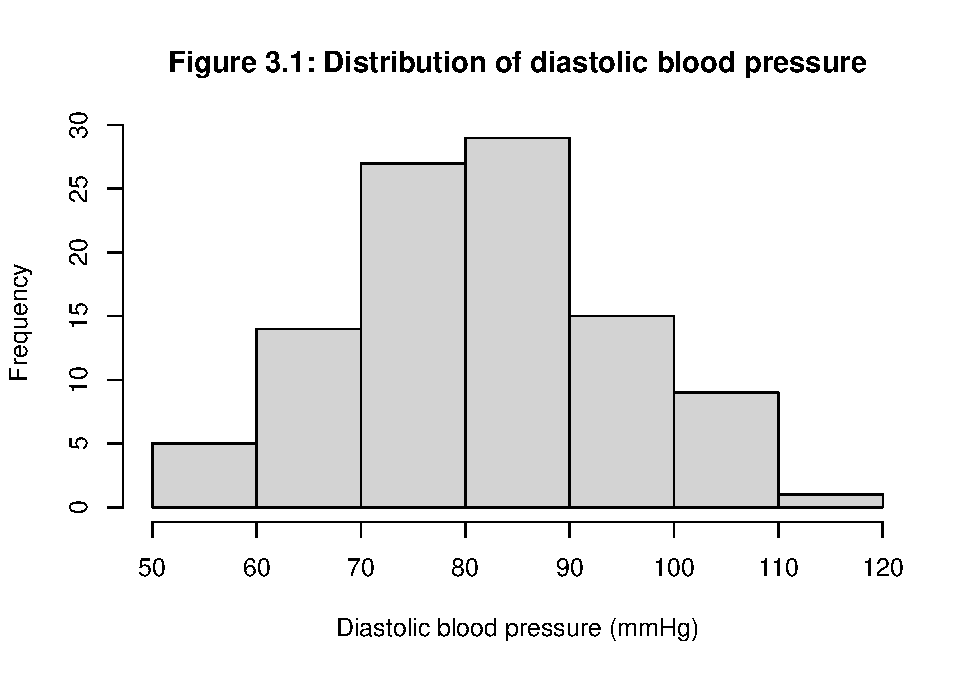
\includegraphics{phcm9795-solutions-R_files/figure-latex/unnamed-chunk-39-1.pdf}

\begin{quote}
The distribution is approximately symmetrical, centered about the mean.
\end{quote}

\begin{enumerate}
\def\labelenumi{\alph{enumi})}
\setcounter{enumi}{1}
\tightlist
\item
  Use R to obtain an estimate of the mean, standard error of the mean and the 95\% confidence interval for the mean diastolic blood pressure.
\end{enumerate}

\begin{Shaded}
\begin{Highlighting}[]
\FunctionTok{descriptives}\NormalTok{(}\AttributeTok{data=}\NormalTok{dbp, }\AttributeTok{vars=}\NormalTok{diabp, }\AttributeTok{se=}\ConstantTok{TRUE}\NormalTok{)}
\end{Highlighting}
\end{Shaded}

\begin{verbatim}
## 
##  DESCRIPTIVES
## 
##  Descriptives                       
##  ────────────────────────────────── 
##                          diabp      
##  ────────────────────────────────── 
##    N                          100   
##    Missing                      0   
##    Mean                  82.23000   
##    Std. error mean       1.301522   
##    Median                83.00000   
##    Standard deviation    13.01522   
##    Minimum               56.00000   
##    Maximum               118.0000   
##  ──────────────────────────────────
\end{verbatim}

\begin{Shaded}
\begin{Highlighting}[]
\FunctionTok{t.test}\NormalTok{(dbp}\SpecialCharTok{$}\NormalTok{diabp)}
\end{Highlighting}
\end{Shaded}

\begin{verbatim}
## 
##  One Sample t-test
## 
## data:  dbp$diabp
## t = 63.18, df = 99, p-value < 2.2e-16
## alternative hypothesis: true mean is not equal to 0
## 95 percent confidence interval:
##  79.6475 84.8125
## sample estimates:
## mean of x 
##     82.23
\end{verbatim}

\begin{quote}
The sample mean is estimated as 82.2 mmHg, and the standard error (SE) of the mean is 1.30 mmHg. The 95\% confidence interval is from 79.6 to 84.8 mmHg.
\end{quote}

\begin{quote}
\emph{Note that the original data have one decimal place. While we could present the mean to two decimal places when reporting the mean, it seems a bit excessive to present a mean blood pressure to two decimal places. Thus we report the mean and 95\% confidence interval for the mean with 1 decimal place.}
\end{quote}

\begin{enumerate}
\def\labelenumi{\alph{enumi})}
\setcounter{enumi}{2}
\tightlist
\item
  What can you say about the population mean from these results? (Include in you answer what is meant by the confidence interval of a mean).
\end{enumerate}

\begin{quote}
We are 95\% confident that true mean of the population from which we sampled lies between 79.6 mmHg and 84.8 mmHg.
\end{quote}

\hypertarget{activity-3.4}{%
\subsection*{Activity 3.4}\label{activity-3.4}}
\addcontentsline{toc}{subsection}{Activity 3.4}

Suppose that a random sample of 81 newborn babies delivered in a hospital located in a poor neighbourhood during the last year had a mean birth weight of 2.7 kg and a standard deviation of 0.9 kg. Calculate the 95\% confidence interval for the unknown population mean. Interpret the 95\% confidence interval.

\begin{quote}
This question asks for a confidence interval to be calculated from summarised data. R does not have an in-built function to do this, but we can use the code presented in the R notes to complete this activitiy.
\end{quote}

\begin{Shaded}
\begin{Highlighting}[]
\NormalTok{ci\_mean }\OtherTok{\textless{}{-}} \ControlFlowTok{function}\NormalTok{(n, mean, sd, }\AttributeTok{width=}\FloatTok{0.95}\NormalTok{, }\AttributeTok{digits=}\DecValTok{3}\NormalTok{)\{}
\NormalTok{  lcl }\OtherTok{\textless{}{-}}\NormalTok{ mean }\SpecialCharTok{{-}} \FunctionTok{qt}\NormalTok{(}\AttributeTok{p=}\NormalTok{(}\DecValTok{1} \SpecialCharTok{{-}}\NormalTok{ (}\DecValTok{1}\SpecialCharTok{{-}}\NormalTok{width)}\SpecialCharTok{/}\DecValTok{2}\NormalTok{), }\AttributeTok{df=}\NormalTok{n}\DecValTok{{-}1}\NormalTok{) }\SpecialCharTok{*}\NormalTok{ sd}\SpecialCharTok{/}\FunctionTok{sqrt}\NormalTok{(n)}
\NormalTok{  ucl }\OtherTok{\textless{}{-}}\NormalTok{ mean }\SpecialCharTok{+} \FunctionTok{qt}\NormalTok{(}\AttributeTok{p=}\NormalTok{(}\DecValTok{1} \SpecialCharTok{{-}}\NormalTok{ (}\DecValTok{1}\SpecialCharTok{{-}}\NormalTok{width)}\SpecialCharTok{/}\DecValTok{2}\NormalTok{), }\AttributeTok{df=}\NormalTok{n}\DecValTok{{-}1}\NormalTok{) }\SpecialCharTok{*}\NormalTok{ sd}\SpecialCharTok{/}\FunctionTok{sqrt}\NormalTok{(n)}
  
  \FunctionTok{print}\NormalTok{(}\FunctionTok{paste0}\NormalTok{(width}\SpecialCharTok{*}\DecValTok{100}\NormalTok{, }\StringTok{"\%"}\NormalTok{, }\StringTok{" CI: "}\NormalTok{, }
               \FunctionTok{format}\NormalTok{(}\FunctionTok{round}\NormalTok{(lcl, }\AttributeTok{digits=}\NormalTok{digits), }\AttributeTok{nsmall =}\NormalTok{ digits),}
               \StringTok{" to "}\NormalTok{, }\FunctionTok{format}\NormalTok{(}\FunctionTok{round}\NormalTok{(ucl, }\AttributeTok{digits=}\NormalTok{digits), }\AttributeTok{nsmall =}\NormalTok{ digits) ))}

\NormalTok{\}}

\FunctionTok{ci\_mean}\NormalTok{(}\AttributeTok{n=}\DecValTok{81}\NormalTok{, }\AttributeTok{mean=}\FloatTok{2.7}\NormalTok{, }\AttributeTok{sd=}\FloatTok{0.9}\NormalTok{, }\AttributeTok{width=}\FloatTok{0.95}\NormalTok{)}
\end{Highlighting}
\end{Shaded}

\begin{verbatim}
## [1] "95% CI: 2.501 to 2.899"
\end{verbatim}

\begin{quote}
We are 95\% confident that the true mean birthweight in the hospital located in a poor neighbourhood lies between 2.5 kg and 2.9 kg.
\end{quote}

\hypertarget{module-3-full-script}{%
\chapter*{Module 3: Full script}\label{module-3-full-script}}
\addcontentsline{toc}{chapter}{Module 3: Full script}

\begin{Shaded}
\begin{Highlighting}[]
\CommentTok{\# Author: Timothy Dobbins}
\CommentTok{\# Date: June, 2022}
\CommentTok{\# Purpose: Learning activities for Module 3}

\FunctionTok{library}\NormalTok{(jmv)}

\CommentTok{\# Activity 3.2}
\CommentTok{\# i: n=25}
\NormalTok{n }\OtherTok{\textless{}{-}} \DecValTok{25}
\NormalTok{se }\OtherTok{\textless{}{-}} \DecValTok{85} \SpecialCharTok{/} \FunctionTok{sqrt}\NormalTok{(n)}
\NormalTok{se}

\NormalTok{mle }\OtherTok{\textless{}{-}} \FloatTok{1.96} \SpecialCharTok{*}\NormalTok{ se}
\NormalTok{mle}

\CommentTok{\# ii: n=100}
\NormalTok{n }\OtherTok{\textless{}{-}} \DecValTok{100}
\NormalTok{se }\OtherTok{\textless{}{-}} \DecValTok{85} \SpecialCharTok{/} \FunctionTok{sqrt}\NormalTok{(n)}
\NormalTok{se}

\NormalTok{mle }\OtherTok{\textless{}{-}} \FloatTok{1.96} \SpecialCharTok{*}\NormalTok{ se}
\NormalTok{mle}

\CommentTok{\# iii: n=625}
\NormalTok{n }\OtherTok{\textless{}{-}} \DecValTok{625}
\NormalTok{se }\OtherTok{\textless{}{-}} \DecValTok{85} \SpecialCharTok{/} \FunctionTok{sqrt}\NormalTok{(n)}
\NormalTok{se}

\NormalTok{mle }\OtherTok{\textless{}{-}} \FloatTok{1.96} \SpecialCharTok{*}\NormalTok{ se}
\NormalTok{mle}

\CommentTok{\# iv: n=3000}
\NormalTok{n }\OtherTok{\textless{}{-}} \DecValTok{3000}
\NormalTok{se }\OtherTok{\textless{}{-}} \DecValTok{85} \SpecialCharTok{/} \FunctionTok{sqrt}\NormalTok{(n)}
\NormalTok{se}

\NormalTok{mle }\OtherTok{\textless{}{-}} \FloatTok{1.96} \SpecialCharTok{*}\NormalTok{ se}
\NormalTok{mle}


\CommentTok{\# Activity 3.3}
\NormalTok{dbp }\OtherTok{\textless{}{-}} \FunctionTok{readRDS}\NormalTok{(}\StringTok{"data/activities/Activity\_S1.4.rds"}\NormalTok{)}

\FunctionTok{hist}\NormalTok{(dbp}\SpecialCharTok{$}\NormalTok{diabp, }
     \AttributeTok{main=}\StringTok{"Figure 3.1: Distribution of diastolic blood pressure"}\NormalTok{, }
     \AttributeTok{xlab=}\StringTok{"Diastolic blood pressure (mmHg)"}\NormalTok{)}

\FunctionTok{descriptives}\NormalTok{(}\AttributeTok{data=}\NormalTok{dbp, }\AttributeTok{vars=}\NormalTok{diabp, }\AttributeTok{se=}\ConstantTok{TRUE}\NormalTok{)}
\FunctionTok{t.test}\NormalTok{(dbp}\SpecialCharTok{$}\NormalTok{diabp)}

\CommentTok{\# Activity 3.4}
\NormalTok{ci\_mean }\OtherTok{\textless{}{-}} \ControlFlowTok{function}\NormalTok{(n, mean, sd, }\AttributeTok{width=}\FloatTok{0.95}\NormalTok{, }\AttributeTok{digits=}\DecValTok{3}\NormalTok{)\{}
\NormalTok{  lcl }\OtherTok{\textless{}{-}}\NormalTok{ mean }\SpecialCharTok{{-}} \FunctionTok{qt}\NormalTok{(}\AttributeTok{p=}\NormalTok{(}\DecValTok{1} \SpecialCharTok{{-}}\NormalTok{ (}\DecValTok{1}\SpecialCharTok{{-}}\NormalTok{width)}\SpecialCharTok{/}\DecValTok{2}\NormalTok{), }\AttributeTok{df=}\NormalTok{n}\DecValTok{{-}1}\NormalTok{) }\SpecialCharTok{*}\NormalTok{ sd}\SpecialCharTok{/}\FunctionTok{sqrt}\NormalTok{(n)}
\NormalTok{  ucl }\OtherTok{\textless{}{-}}\NormalTok{ mean }\SpecialCharTok{+} \FunctionTok{qt}\NormalTok{(}\AttributeTok{p=}\NormalTok{(}\DecValTok{1} \SpecialCharTok{{-}}\NormalTok{ (}\DecValTok{1}\SpecialCharTok{{-}}\NormalTok{width)}\SpecialCharTok{/}\DecValTok{2}\NormalTok{), }\AttributeTok{df=}\NormalTok{n}\DecValTok{{-}1}\NormalTok{) }\SpecialCharTok{*}\NormalTok{ sd}\SpecialCharTok{/}\FunctionTok{sqrt}\NormalTok{(n)}
  
  \FunctionTok{print}\NormalTok{(}\FunctionTok{paste0}\NormalTok{(width}\SpecialCharTok{*}\DecValTok{100}\NormalTok{, }\StringTok{"\%"}\NormalTok{, }\StringTok{" CI: "}\NormalTok{, }
               \FunctionTok{format}\NormalTok{(}\FunctionTok{round}\NormalTok{(lcl, }\AttributeTok{digits=}\NormalTok{digits), }\AttributeTok{nsmall =}\NormalTok{ digits),}
               \StringTok{" to "}\NormalTok{, }\FunctionTok{format}\NormalTok{(}\FunctionTok{round}\NormalTok{(ucl, }\AttributeTok{digits=}\NormalTok{digits), }\AttributeTok{nsmall =}\NormalTok{ digits) ))}

\NormalTok{\}}

\FunctionTok{ci\_mean}\NormalTok{(}\AttributeTok{n=}\DecValTok{81}\NormalTok{, }\AttributeTok{mean=}\FloatTok{2.7}\NormalTok{, }\AttributeTok{sd=}\FloatTok{0.9}\NormalTok{, }\AttributeTok{width=}\FloatTok{0.95}\NormalTok{)}
\end{Highlighting}
\end{Shaded}

\hypertarget{module-4-solutions-to-learning-activities}{%
\chapter*{Module 4: Solutions to Learning Activities}\label{module-4-solutions-to-learning-activities}}
\addcontentsline{toc}{chapter}{Module 4: Solutions to Learning Activities}

\hypertarget{activity-4.1}{%
\subsection*{Activity 4.1}\label{activity-4.1}}
\addcontentsline{toc}{subsection}{Activity 4.1}

In each of the following situations, what decision should be made about the null hypothesis if the researcher indicates that:

\begin{enumerate}
\def\labelenumi{\alph{enumi})}
\tightlist
\item
  P \textless{} 0.01
\end{enumerate}

\begin{quote}
There is strong evidence against the null hypothesis.
\end{quote}

\begin{enumerate}
\def\labelenumi{\alph{enumi})}
\setcounter{enumi}{1}
\tightlist
\item
  P \textgreater{} 0.05
\end{enumerate}

\begin{quote}
There is weak or little evidence against the null hypothesis - but the researchers should be advised to provide the actual P-value, not just P \textgreater{} 0.05.
\end{quote}

\begin{enumerate}
\def\labelenumi{\alph{enumi})}
\setcounter{enumi}{2}
\tightlist
\item
  `ns' indicating not significant
\end{enumerate}

\begin{quote}
Traditionally, `ns' stands for not significant (for the set level of significance mentioned in the study, usually 0.05). You might still come across this term in some journal articles but this is not best practice for most journals these days. Researchers should always state the P-value (not just whether or not it was significant).
\end{quote}

\begin{enumerate}
\def\labelenumi{\alph{enumi})}
\setcounter{enumi}{3}
\tightlist
\item
  significant differences exist
\end{enumerate}

\begin{quote}
This would imply that the P-value is less than the set level of significance mentioned in the study (usually, 0.05). As such, we would conclude that there was evidence against the null hypothesis. However, the researchers should be advised to always state the P-value (not just whether or not it was significant).
\end{quote}

\hypertarget{activity-4.2}{%
\subsection*{Activity 4.2}\label{activity-4.2}}
\addcontentsline{toc}{subsection}{Activity 4.2}

For the following hypothetical situations, formulate the null hypothesis and alternative hypothesis and write a conclusion about the study results:

\begin{enumerate}
\def\labelenumi{\alph{enumi})}
\tightlist
\item
  A study was conducted to investigate whether the mean systolic blood pressure of males aged 40 to 60 years was different to the mean systolic blood pressure of females aged 40 to 60 years. The result of the study was that the mean systolic blood pressure was higher in males by 5.1 mmHg (95\% CI 2.4 to 7.6; P = 0.008).
\end{enumerate}

\begin{quote}
H\textsubscript{0}: There is no difference in the mean systolic blood pressure between males aged 40-60 years and females aged 40-60 years.
\end{quote}

\begin{quote}
H\textsubscript{A}: There is a difference in the mean systolic blood pressure between males aged 40-60 years and females aged 40 to 60 years.
\end{quote}

\begin{quote}
Conclusion: The mean SBP was 5.1 mmHg (95\% CI: 2.4 to 7.6 mmHg) higher in males aged 40-60 years compared to females aged 40-60 years. The P value is 0.008 which provides strong evidence against the null hypothesis. Therefore, we can conclude that there is a difference in the mean SBP of males and females aged 40-60 years.
\end{quote}

\begin{enumerate}
\def\labelenumi{\alph{enumi})}
\setcounter{enumi}{1}
\tightlist
\item
  A case-control study was conducted to investigate the association between obesity and breast cancer. The researchers found an OR of 3.21 (95\% CI 1.15 to 8.47; P = 0.03).
\end{enumerate}

\begin{quote}
H\textsubscript{0}: There is no association between obesity and breast cancer.
{[}A more formal way of saying this is that there is no difference in the odds of exposure to obesity among cases of breast cancer and controls i.e.~OR = 1{]}.
\end{quote}

\begin{quote}
H\textsubscript{A}: There is an association between obesity and breast cancer.
{[}A more formal way of saying this is that there is a difference in the odds of exposure to obesity among cases and controls i.e.~OR ≠ 1{]}.
\end{quote}

\begin{quote}
Conclusion: The odds ratio is estimated as 3.21, indicating a positive association between the study factor of obesity and the outcome of breast cancer. The 95\% CI is 1.15 to 8.47 and excludes the null value of no association (i.e.~OR = 1). The P value is 0.03 which provides evidence against the null hypothesis. Therefore, we can conclude that there is a positive association between obesity and breast cancer.
\end{quote}

\begin{enumerate}
\def\labelenumi{\alph{enumi})}
\setcounter{enumi}{2}
\tightlist
\item
  A cohort study investigated the relationship between eating a healthy diet and the incidence of influenza infection among adults aged 20 to 60 years. The results were RR = 0.88 (95\% CI 0.65 to 1.50; P = 0.2).
\end{enumerate}

\begin{quote}
H\textsubscript{0}: There is no association between influenza infection and a healthy diet among adults aged 20-60 years.
{[}A more formal way of saying this is that there is no difference in the risk of influenza infection among adults aged 20-60 years who have a healthy diet compared to those who do not have a healthy diet. i.e.~RR = 1{]}.
\end{quote}

\begin{quote}
H\textsubscript{A}: There is an association between influenza infection and a healthy diet among adults aged 20-60 years.
{[}A more formal way of saying this is that there is a difference in the risk of influenza infection among adults aged 20-60 years who have a healthy diet compared to those who do not have a healthy diet. i.e.~RR ≠ 1{]}.
\end{quote}

\begin{quote}
Conclusion: The relative risk is estimated as 0.88, indicating a protective association between the study factor of healthy diet and the outcome factor of influenza infection among adults aged 20 to 60 years. However, the 95\% confidence interval includes the null value of 1.0 (no association). The P value is 0.2, which means there is no evidence against the null hypothesis. Thus, we can conclude that there is no evidence of an association between a healthy diet and influenza infection among adults aged 20 to 60 years.
\end{quote}

\hypertarget{activity-4.3}{%
\subsection*{Activity 4.3}\label{activity-4.3}}
\addcontentsline{toc}{subsection}{Activity 4.3}

A pilot study was conducted to compare the mean daily energy intake of women aged 25 to 30 years with the recommended intake of 7750 kJ/day. In this study, the average daily energy intake over 10 days was recorded for 12 healthy women of that age group. The data are in the Excel file Activity\_4.3.xls. Import the file into R for this activity.

\begin{enumerate}
\def\labelenumi{\alph{enumi})}
\tightlist
\item
  State the research question
\end{enumerate}

\begin{quote}
Is the mean daily energy intake of women aged 25-30 years different to the recommended daily intake of 7750 kJ/day?
\end{quote}

\begin{enumerate}
\def\labelenumi{\alph{enumi})}
\setcounter{enumi}{1}
\tightlist
\item
  Formulate the null hypothesis
\end{enumerate}

\begin{quote}
H\textsubscript{0}: the mean daily energy intake of women aged 25-30 years is the same as the recommended daily intake of 7750 kJ/day.
\end{quote}

\begin{enumerate}
\def\labelenumi{\alph{enumi})}
\setcounter{enumi}{2}
\tightlist
\item
  Formulate the alternative hypothesis
\end{enumerate}

\begin{quote}
H\textsubscript{A}: the mean daily energy intake of women aged 25-30 years is not same as the recommended daily intake of 7750 kJ/day.
\end{quote}

\begin{enumerate}
\def\labelenumi{\alph{enumi})}
\setcounter{enumi}{3}
\tightlist
\item
  Analyse the data and report your conclusions
\end{enumerate}

\begin{Shaded}
\begin{Highlighting}[]
\FunctionTok{library}\NormalTok{(readxl)}
\FunctionTok{library}\NormalTok{(jmv)}

\NormalTok{pilot }\OtherTok{\textless{}{-}} \FunctionTok{read\_excel}\NormalTok{(}\StringTok{"data/activities/Activity\_S4.3.xls"}\NormalTok{)}
\FunctionTok{summary}\NormalTok{(pilot)}
\end{Highlighting}
\end{Shaded}

\begin{verbatim}
##      Energy    
##  Min.   :5260  
##  1st Qu.:6045  
##  Median :6674  
##  Mean   :6856  
##  3rd Qu.:7642  
##  Max.   :8770
\end{verbatim}

\begin{quote}
As we are comparing a continuous distribution to a hypothesised mean, we will use a one-sample t-test to conduct this analysis. As the one-sample t-test assumes our data follow a Normal distribution, we should assess this using a histogram.
\end{quote}

\begin{Shaded}
\begin{Highlighting}[]
\FunctionTok{hist}\NormalTok{(pilot}\SpecialCharTok{$}\NormalTok{Energy, }\AttributeTok{main=}\StringTok{"Daily energy intake of pilot participants"}\NormalTok{, }\AttributeTok{xlab=}\StringTok{"Energy (kJ)"}\NormalTok{)}
\end{Highlighting}
\end{Shaded}

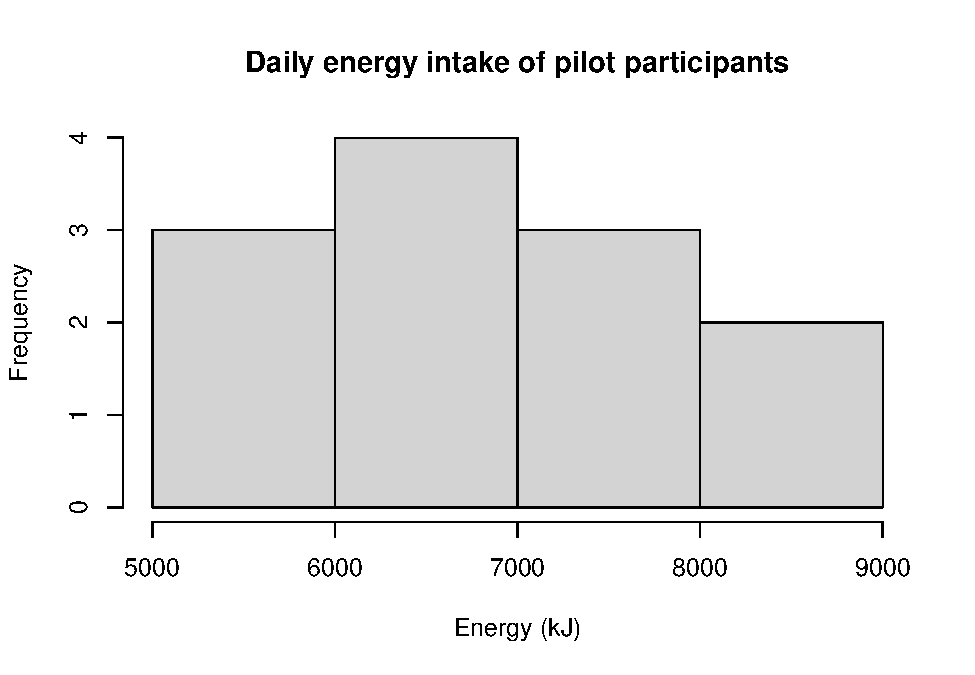
\includegraphics{phcm9795-solutions-R_files/figure-latex/unnamed-chunk-44-1.pdf}

\begin{quote}
It is very difficult to assess the shape of a distribution with only 12 observations, but here we can see that the distribution looks roughly symmetric. In this case, we will assume Normality.
\end{quote}

\begin{quote}
The one-sample t-test is conducted as below, to compare the variable Energy to the hypothesised mean of 7750 kJ/day:
\end{quote}

\begin{Shaded}
\begin{Highlighting}[]
\FunctionTok{t.test}\NormalTok{(pilot}\SpecialCharTok{$}\NormalTok{Energy, }\AttributeTok{mu=}\DecValTok{7750}\NormalTok{)}
\end{Highlighting}
\end{Shaded}

\begin{verbatim}
## 
##  One Sample t-test
## 
## data:  pilot$Energy
## t = -2.7141, df = 11, p-value = 0.02014
## alternative hypothesis: true mean is not equal to 7750
## 95 percent confidence interval:
##  6131.023 7580.977
## sample estimates:
## mean of x 
##      6856
\end{verbatim}

\begin{quote}
The one-sample t-test output shows that the mean daily energy intake of the 12 women is 6856 kJ (95\% CI: 6131 to 7581 kJ). There is evidence (t = −2.71 with 11 DF, P = 0.02) that the mean daily energy intake of women aged 25-30 years is lower than the recommended daily intake of 7750 kJ/day.
\end{quote}

\hypertarget{activity-4.4}{%
\subsection*{Activity 4.4}\label{activity-4.4}}
\addcontentsline{toc}{subsection}{Activity 4.4}

Which procedure gives the researcher the better chance of rejecting a null hypothesis?

\begin{enumerate}
\def\labelenumi{\alph{enumi})}
\tightlist
\item
  comparing the data-based p-value with the level of significance at 5\%
\item
  comparing the 95\% CI with a nominated value
\item
  neither procedure
\end{enumerate}

\begin{quote}
Both `a' and `b' would give the same chance to reject the null hypothesis. This is because both `a' and `b' are giving you the same information in a different way. In `a' you will get the probability of observing the difference you see in your data by chance and if it is \textless0.05 you will reject the null hypothesis at the 5\% level. Whereas in `b' you will see whether the null value (value of no difference) lies within the range which you are 95\% confident contains the true value. If the null value falls outside the 95\% CI, you would have less than 5\% (100-95 = 5\%) probability seeing the observed difference in your data if there were no difference.
\end{quote}

\hypertarget{activity-4.5}{%
\subsection*{Activity 4.5}\label{activity-4.5}}
\addcontentsline{toc}{subsection}{Activity 4.5}

Setting the significance level at P \textless{} 0.10 instead of the more usual P \textless{} 0.05 increases the likelihood of:

\begin{enumerate}
\def\labelenumi{\alph{enumi})}
\tightlist
\item
  a Type I error
\item
  a Type II error
\item
  rejecting the null hypothesis
\item
  Not rejecting the null hypothesis
\end{enumerate}

\begin{quote}
Setting the significance level cut-off at 0.10 instead of the more usual 0.05 increases the likelihood of
\textbf{a. a Type I error} and \textbf{c.~rejecting the null hypothesis}.
\end{quote}

\begin{quote}
The cut-off of 0.10 increases the chance of a type I error from 5\% to 10\% (the chance of making a Type I error is the same as the significance level). If the significance level is higher, then there higher probability of rejecting the null hypothesis if there no effect in reality.
\end{quote}

\hypertarget{activity-4.6}{%
\subsection*{Activity 4.6}\label{activity-4.6}}
\addcontentsline{toc}{subsection}{Activity 4.6}

For a fixed sample size setting the significance level at a very extreme cut-off such as P \textless{} 0.001 increases the chances of:

\begin{enumerate}
\def\labelenumi{\alph{enumi})}
\tightlist
\item
  obtaining a significant result
\item
  rejecting the null hypothesis
\item
  a Type I error
\item
  a Type II error
\end{enumerate}

\begin{quote}
Setting the significance level at a very extreme cut-off (such as 0.001) increases the chances of: \textbf{d.~a Type II error}.
\end{quote}

\begin{quote}
For a given sample, if the significance level is set very small it will make it harder to find evidence against the null hypothesis. In other words, it will be difficult to detect an effect if an effect exists in reality. In other words, the probability of type II error will increase: you will not be able to reject the null hypothesis when a real difference exists.
\end{quote}

\hypertarget{module-4-full-script}{%
\chapter*{Module 4: Full script}\label{module-4-full-script}}
\addcontentsline{toc}{chapter}{Module 4: Full script}

\begin{Shaded}
\begin{Highlighting}[]
\CommentTok{\# Author: Timothy Dobbins}
\CommentTok{\# Date: June, 2022}
\CommentTok{\# Purpose: Learning activities for Module 4}

\FunctionTok{library}\NormalTok{(readxl)}
\FunctionTok{library}\NormalTok{(jmv)}

\NormalTok{pilot }\OtherTok{\textless{}{-}} \FunctionTok{read\_excel}\NormalTok{(}\StringTok{"data/activities/Activity\_S4.3.xls"}\NormalTok{)}
\FunctionTok{hist}\NormalTok{(pilot}\SpecialCharTok{$}\NormalTok{Energy, }\AttributeTok{main=}\StringTok{"Daily energy intake of pilot participants"}\NormalTok{, }\AttributeTok{xlab=}\StringTok{"Energy (kJ)"}\NormalTok{)}

\FunctionTok{descriptives}\NormalTok{(pilot)}

\FunctionTok{t.test}\NormalTok{(pilot}\SpecialCharTok{$}\NormalTok{Energy, }\AttributeTok{mu=}\DecValTok{7750}\NormalTok{)}
\end{Highlighting}
\end{Shaded}

\hypertarget{module-5-solutions-to-learning-activities}{%
\chapter*{Module 5: Solutions to Learning Activities}\label{module-5-solutions-to-learning-activities}}
\addcontentsline{toc}{chapter}{Module 5: Solutions to Learning Activities}

\hypertarget{activity-5.1}{%
\subsection*{Activity 5.1}\label{activity-5.1}}
\addcontentsline{toc}{subsection}{Activity 5.1}

Indicate what type of t-test could be used to analyse the data from the following studies and provide reasons:

\begin{enumerate}
\def\labelenumi{\alph{enumi})}
\tightlist
\item
  A total of 60 university students are randomly assigned to undergo either behaviour therapy or Gestalt therapy. After twenty therapeutic sessions, each student earns a score on a mental health questionnaire.
\end{enumerate}

\begin{quote}
An independent samples t-test could be used because the two groups (behaviour therapy vs Gestalt therapy) are independent. The mental health scores would need to be normally distributed in each group.
\end{quote}

\begin{enumerate}
\def\labelenumi{\alph{enumi})}
\setcounter{enumi}{1}
\tightlist
\item
  A researcher wishes to determine whether attendance at a day care centre increases the scores of three year old twins on a motor skills test. Random assignment is used to decide which member from each of 30 pairs of twins attends the day care centre and which member stays at home.
\end{enumerate}

\begin{quote}
This is a twin pair study where one member of a twin is allocated to day care and the other member to stay at home. This is an example of an individually matched study and so a paired t-test is appropriate.
\end{quote}

\begin{enumerate}
\def\labelenumi{\alph{enumi})}
\setcounter{enumi}{2}
\tightlist
\item
  A child psychologist assigns aggression scores to each of 10 children during two 60 minute observation periods separated by an intervening exposure to a series of violent TV cartoons.
\end{enumerate}

\begin{quote}
The same children are scored twice (before and after the intervention), thus it is a paired design and a paired t-test is appropriate.
\end{quote}

\begin{enumerate}
\def\labelenumi{\alph{enumi})}
\setcounter{enumi}{3}
\tightlist
\item
  A marketing researcher measures 100 doctors' reports of the number of their patients asking them about a particular drug during the month before and the month after a major advertising campaign.
\end{enumerate}

\begin{quote}
The doctors' reports are paired because they report before and after an intervention. Therefore, a paired t-test is appropriate.
\end{quote}

\hypertarget{activity-5.2}{%
\subsection*{Activity 5.2}\label{activity-5.2}}
\addcontentsline{toc}{subsection}{Activity 5.2}

A study was conducted to compare haemoglobin levels in the blood of children with and without cystic fibrosis. It is known that haemoglobin levels are normally distributed in children. The study results are given below:

\begin{longtable}[]{@{}lll@{}}
\caption{Table 1: Summary of haemoglobin (g/dL)}\tabularnewline
\toprule()
Statistic & Children without CF & Children with CF \\
\midrule()
\endfirsthead
\toprule()
Statistic & Children without CF & Children with CF \\
\midrule()
\endhead
n & 12 & 15 \\
Mean & 19.9 & 13.9 \\
SD (SE) & 5.9 (1.7) & 6.2 (1.6) \\
\bottomrule()
\end{longtable}

\begin{enumerate}
\def\labelenumi{\alph{enumi})}
\tightlist
\item
  State the appropriate null hypothesis and alternate hypothesis
\end{enumerate}

\begin{quote}
The null hypothesis: The mean haemoglobin level of children with cystic fibrosis is the same as the mean haemoglobin level of children without cystic fibrosis.
\end{quote}

\begin{quote}
The alternative hypothesis: The mean haemoglobin level of children with cystic fibrosis is different to the mean haemoglobin level of children without cystic fibrosis.
\end{quote}

\begin{enumerate}
\def\labelenumi{\alph{enumi})}
\setcounter{enumi}{1}
\tightlist
\item
  Use R to conduct an appropriate statistical test to evaluate the null hypothesis. Are the assumptions for the test met for this analysis to be valid?
\end{enumerate}

\begin{quote}
An independent samples t-test could be carried out to evaluate the study hypothesis because the data have been collected from 2 independent groups of children (children with and children without cystic fibrosis).
\end{quote}

\begin{quote}
The assumption of independence is met. The outcome variable is continuous and the data are approximately normally distributed in the underlying population (as mentioned in the question).
\end{quote}

\begin{quote}
We are provided with summarised data (i.e.~means and standard deviations in each group), and not individual data. Therefore, we cannot use the standard \texttt{t.test()} function. The \texttt{BSDA} package has the \texttt{tsum.test()} function that can perform a t-test using summarised data.
\end{quote}

\begin{Shaded}
\begin{Highlighting}[]
\CommentTok{\# If necessary, install the BSDA package:}
\CommentTok{\# install.packages("BSDA")}
\FunctionTok{library}\NormalTok{(BSDA)}
\end{Highlighting}
\end{Shaded}

\begin{verbatim}
## Loading required package: lattice
\end{verbatim}

\begin{verbatim}
## 
## Attaching package: 'BSDA'
\end{verbatim}

\begin{verbatim}
## The following object is masked from 'package:datasets':
## 
##     Orange
\end{verbatim}

\begin{Shaded}
\begin{Highlighting}[]
\CommentTok{\# Calculate difference in means by hand:}
\FloatTok{19.9} \SpecialCharTok{{-}} \FloatTok{13.9}
\end{Highlighting}
\end{Shaded}

\begin{verbatim}
## [1] 6
\end{verbatim}

\begin{Shaded}
\begin{Highlighting}[]
\CommentTok{\# t{-}test assuming equal variance}
\FunctionTok{tsum.test}\NormalTok{(}\AttributeTok{mean.x=}\FloatTok{19.9}\NormalTok{, }\AttributeTok{s.x=}\FloatTok{5.9}\NormalTok{, }\AttributeTok{n.x=}\DecValTok{12}\NormalTok{,}
          \AttributeTok{mean.y=}\FloatTok{13.9}\NormalTok{, }\AttributeTok{s.y=}\FloatTok{6.2}\NormalTok{, }\AttributeTok{n.y=}\DecValTok{15}\NormalTok{,}
          \AttributeTok{mu=}\DecValTok{0}\NormalTok{, }\AttributeTok{alternative=}\StringTok{"two.sided"}\NormalTok{, }\AttributeTok{var.equal =} \ConstantTok{TRUE}\NormalTok{)}
\end{Highlighting}
\end{Shaded}

\begin{verbatim}
## 
##  Standard Two-Sample t-Test
## 
## data:  Summarized x and y
## t = 2.5523, df = 25, p-value = 0.01719
## alternative hypothesis: true difference in means is not equal to 0
## 95 percent confidence interval:
##   1.158367 10.841633
## sample estimates:
## mean of x mean of y 
##      19.9      13.9
\end{verbatim}

\begin{quote}
As the two standard deviations are similar, we can assume equal variances. There is evidence that the mean haemoglobin level is lower in children with cystic fibrosis (13.9 g/dL) than children without cystic fibrosis (19.9 g/dL; t=2.55 with 25 df, P=0.02). The difference in means is estimated as 6.0 g/dL (95\% CI: 1.2 to 10.8).
\end{quote}

\hypertarget{activity-5.3}{%
\subsection*{Activity 5.3}\label{activity-5.3}}
\addcontentsline{toc}{subsection}{Activity 5.3}

A randomised controlled trial (RCT) was carried out to investigate the effect of a new tablet supplement in increasing the hematocrit (\%) value in anaemic participants. In the study, hematocrit was measured as the proportion of blood that is made up of red blood cells. Hematocrit levels are often lower in anaemic people who do not have sufficient healthy red blood cells. In the RCT, 33 people in the intervention group received the new supplement and 31 people in the control group received standard care (i.e.~the usual supplement was given). After 4 weeks, hematocrit values were measured as shown in the R file \texttt{ActivityS5.3.rds}. In the community, hematocrit levels are normally distributed.

\begin{enumerate}
\def\labelenumi{\alph{enumi})}
\tightlist
\item
  State the research question and frame it as a null hypothesis.
\end{enumerate}

\begin{quote}
Research question: Do anaemic patients randomised to take a new supplement have different hematocrit values compared to the anaemic patients randomised to receive the usual care?
\end{quote}

\begin{quote}
Null hypothesis: There is no difference in the mean hematocrit value in patients randomised to take the new supplement and patients randomised to the control group.
\end{quote}

\begin{enumerate}
\def\labelenumi{\alph{enumi})}
\setcounter{enumi}{1}
\tightlist
\item
  Use R to conduct an appropriate statistical test to answer the research question. Before using the test, check the data to see if the assumptions required for the test are met. Obtain a box plot to obtain an estimate of the centre and spread of the data for each group.
\end{enumerate}

\begin{quote}
The appropriate test is an independent sample t-test. The assumptions for independent sample t-test are:
\end{quote}

\begin{quote}
\begin{itemize}
\tightlist
\item
  The two groups are independent
\item
  The measurements are independent
\item
  The outcome variable must be continuous and must be normally distributed in each group
\end{itemize}
\end{quote}

\begin{quote}
Based on the study design (RCT with 33 people in the intervention, 31 in the control group and the hematocrit level was measured only once per person) we can say that the first two assumptions are met.
\end{quote}

\begin{quote}
The outcome variable is the proportion of blood that is made up of red blood cells which can be assumed to be continuous.
\end{quote}

\begin{quote}
The histograms and box-plots in Figure 2 (below) show that the data are approximately normally distributed in the intervention group but there is a slight deviation from normality observed in the control group. This is indicated by some deviation from symmetry of the histogram, although there are no influential outliers.
\end{quote}

\begin{quote}
It is mentioned in the question that the outcome variable is normally distributed in the general population. Because the t-test is robust to some degree of non-normality with absence of influential outliers, we could say that the third assumption is also met.
\end{quote}

\begin{quote}
We obtained descriptive statistics for both the intervention and control groups using \texttt{descriptives()} function from the \texttt{jmv} package. From the descriptive statistics we can see that standard deviation of the intervention group (1.57) is slightly larger than in the control group (0.99). Inspection of Figures \ref{fig:haemplot-1} and \ref{fig:haemplot-2} also indicates more variability in the intervention group. Therefore, it may not be reasonable to assume that the variances are equal. In this case, we will use independent sample t-test based on unequal variance assumption.
\end{quote}

\begin{Shaded}
\begin{Highlighting}[]
\CommentTok{\# Activity 5.3}
\FunctionTok{library}\NormalTok{(jmv)}

\NormalTok{anaemia }\OtherTok{\textless{}{-}} \FunctionTok{readRDS}\NormalTok{(}\StringTok{"data/activities/Activity\_S5.3.rds"}\NormalTok{)}

\FunctionTok{descriptives}\NormalTok{(}\AttributeTok{data=}\NormalTok{anaemia, }\AttributeTok{vars=}\NormalTok{hematocrit,}
             \AttributeTok{splitBy =}\NormalTok{ group,}
             \AttributeTok{skew =} \ConstantTok{TRUE}\NormalTok{)}
\end{Highlighting}
\end{Shaded}

\begin{verbatim}
## 
##  DESCRIPTIVES
## 
##  Descriptives                                           
##  ────────────────────────────────────────────────────── 
##                           group            hematocrit   
##  ────────────────────────────────────────────────────── 
##    N                      Intervention             33   
##                           Standard care            31   
##    Missing                Intervention              0   
##                           Standard care             0   
##    Mean                   Intervention       32.43636   
##                           Standard care      31.64516   
##    Median                 Intervention       32.30000   
##                           Standard care      31.80000   
##    Standard deviation     Intervention       1.570991   
##                           Standard care     0.9871976   
##    Minimum                Intervention       29.60000   
##                           Standard care      29.80000   
##    Maximum                Intervention       36.10000   
##                           Standard care      33.20000   
##    Skewness               Intervention      0.2816846   
##                           Standard care    -0.1638483   
##    Std. error skewness    Intervention      0.4086354   
##                           Standard care     0.4205365   
##  ──────────────────────────────────────────────────────
\end{verbatim}

\begin{Shaded}
\begin{Highlighting}[]
\CommentTok{\# Plotting by group using the method from Module 2:}
\NormalTok{anaemia\_i }\OtherTok{\textless{}{-}} \FunctionTok{subset}\NormalTok{(anaemia, group}\SpecialCharTok{==}\StringTok{"Intervention"}\NormalTok{)}
\NormalTok{anaemia\_sc }\OtherTok{\textless{}{-}} \FunctionTok{subset}\NormalTok{(anaemia, group}\SpecialCharTok{==}\StringTok{"Standard care"}\NormalTok{)}

\CommentTok{\# Set the graphics parameters to plot 2 rows and 2 columns:}
\FunctionTok{par}\NormalTok{(}\AttributeTok{mfrow=}\FunctionTok{c}\NormalTok{(}\DecValTok{2}\NormalTok{,}\DecValTok{2}\NormalTok{))}

\CommentTok{\# Specify each plot separately}
\FunctionTok{hist}\NormalTok{(anaemia\_i}\SpecialCharTok{$}\NormalTok{hematocrit, }\AttributeTok{xlab=}\StringTok{"Hematocrit"}\NormalTok{, }\AttributeTok{main=}\StringTok{"Intervention"}\NormalTok{)}
\FunctionTok{hist}\NormalTok{(anaemia\_sc}\SpecialCharTok{$}\NormalTok{hematocrit, }\AttributeTok{xlab=}\StringTok{"Hematocrit"}\NormalTok{, }\AttributeTok{main=}\StringTok{"Standard care"}\NormalTok{)}

\FunctionTok{boxplot}\NormalTok{(anaemia\_i}\SpecialCharTok{$}\NormalTok{hematocrit, }\AttributeTok{ylab=}\StringTok{"Hematocrit"}\NormalTok{, }\AttributeTok{main=}\StringTok{"Intervention"}\NormalTok{)}
\FunctionTok{boxplot}\NormalTok{(anaemia\_sc}\SpecialCharTok{$}\NormalTok{hematocrit, }\AttributeTok{ylab=}\StringTok{"Hematocrit"}\NormalTok{, }\AttributeTok{main=}\StringTok{"Standard care"}\NormalTok{)}
\end{Highlighting}
\end{Shaded}

\begin{figure}
\centering
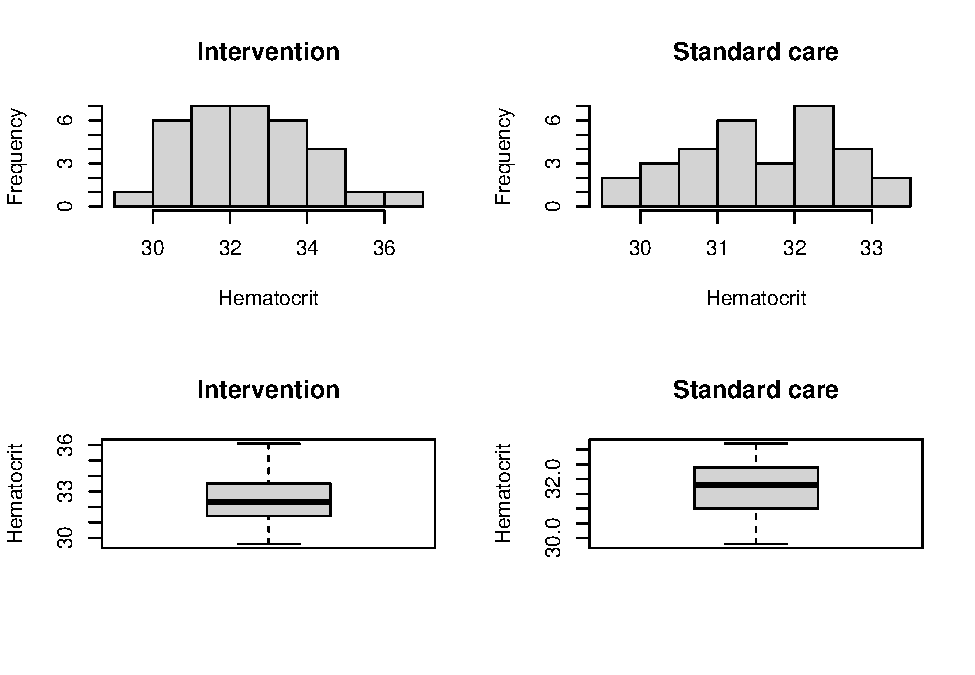
\includegraphics{phcm9795-solutions-R_files/figure-latex/haemplot-1-1.pdf}
\caption{\label{fig:haemplot-1}Graphical summaries of hematocrit by treatment group}
\end{figure}

\begin{Shaded}
\begin{Highlighting}[]
\CommentTok{\# Reset graphics parameters}
\FunctionTok{par}\NormalTok{(}\AttributeTok{mfrow=}\FunctionTok{c}\NormalTok{(}\DecValTok{1}\NormalTok{,}\DecValTok{1}\NormalTok{))}
\end{Highlighting}
\end{Shaded}

Note that the histograms and boxplots use different scales. We can standardise the scale limits using ``xlim'' and ``ylim'' by specifying the lower and upper bounds of the x- and y-axis:

\begin{Shaded}
\begin{Highlighting}[]
\FunctionTok{par}\NormalTok{(}\AttributeTok{mfrow=}\FunctionTok{c}\NormalTok{(}\DecValTok{2}\NormalTok{,}\DecValTok{2}\NormalTok{))}

\FunctionTok{hist}\NormalTok{(anaemia\_i}\SpecialCharTok{$}\NormalTok{hematocrit, }\AttributeTok{xlab=}\StringTok{"Hematocrit"}\NormalTok{, }\AttributeTok{main=}\StringTok{"Intervention"}\NormalTok{,}
     \AttributeTok{xlim=}\FunctionTok{c}\NormalTok{(}\DecValTok{28}\NormalTok{, }\DecValTok{38}\NormalTok{))}
\FunctionTok{hist}\NormalTok{(anaemia\_sc}\SpecialCharTok{$}\NormalTok{hematocrit, }\AttributeTok{xlab=}\StringTok{"Hematocrit"}\NormalTok{, }\AttributeTok{main=}\StringTok{"Standard care"}\NormalTok{,}
     \AttributeTok{xlim=}\FunctionTok{c}\NormalTok{(}\DecValTok{28}\NormalTok{, }\DecValTok{38}\NormalTok{))}

\FunctionTok{boxplot}\NormalTok{(anaemia\_i}\SpecialCharTok{$}\NormalTok{hematocrit, }\AttributeTok{ylab=}\StringTok{"Hematocrit"}\NormalTok{, }\AttributeTok{main=}\StringTok{"Intervention"}\NormalTok{,}
        \AttributeTok{ylim=}\FunctionTok{c}\NormalTok{(}\DecValTok{28}\NormalTok{, }\DecValTok{38}\NormalTok{))}
\FunctionTok{boxplot}\NormalTok{(anaemia\_sc}\SpecialCharTok{$}\NormalTok{hematocrit, }\AttributeTok{ylab=}\StringTok{"Hematocrit"}\NormalTok{, }\AttributeTok{main=}\StringTok{"Standard care"}\NormalTok{,}
        \AttributeTok{ylim=}\FunctionTok{c}\NormalTok{(}\DecValTok{28}\NormalTok{, }\DecValTok{38}\NormalTok{))}
\end{Highlighting}
\end{Shaded}

\begin{figure}
\centering
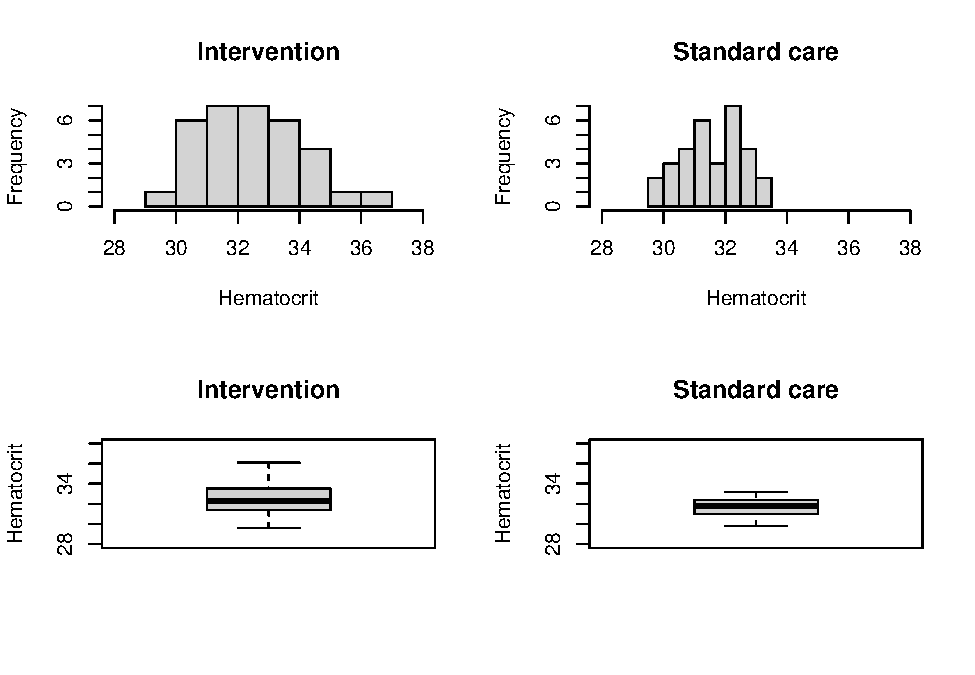
\includegraphics{phcm9795-solutions-R_files/figure-latex/haemplot-2-1.pdf}
\caption{\label{fig:haemplot-2}Graphical summaries of hematocrit by treatment group}
\end{figure}

\begin{Shaded}
\begin{Highlighting}[]
\CommentTok{\# Reset graphics parameters}
\FunctionTok{par}\NormalTok{(}\AttributeTok{mfrow=}\FunctionTok{c}\NormalTok{(}\DecValTok{1}\NormalTok{,}\DecValTok{1}\NormalTok{))}
\end{Highlighting}
\end{Shaded}

\begin{enumerate}
\def\labelenumi{\alph{enumi})}
\setcounter{enumi}{2}
\tightlist
\item
  Run your statistical test.
\end{enumerate}

\begin{Shaded}
\begin{Highlighting}[]
\CommentTok{\# Welch\textquotesingle{}s t{-}test}
\FunctionTok{ttestIS}\NormalTok{(}\AttributeTok{data=}\NormalTok{anaemia, }\AttributeTok{vars=}\NormalTok{hematocrit, }\AttributeTok{group=}\NormalTok{group, }\AttributeTok{meanDiff=}\ConstantTok{TRUE}\NormalTok{, }\AttributeTok{ci=}\ConstantTok{TRUE}\NormalTok{, }\AttributeTok{welchs=}\ConstantTok{TRUE}\NormalTok{)}
\end{Highlighting}
\end{Shaded}

\begin{verbatim}
## 
##  INDEPENDENT SAMPLES T-TEST
## 
##  Independent Samples T-Test                                                                                                       
##  ──────────────────────────────────────────────────────────────────────────────────────────────────────────────────────────────── 
##                                 Statistic    df          p            Mean difference    SE difference    Lower        Upper      
##  ──────────────────────────────────────────────────────────────────────────────────────────────────────────────────────────────── 
##    hematocrit    Student's t     2.394370    62.00000    0.0196861          0.7912023        0.3304428    0.1306566    1.451748   
##                  Welch's t       2.427577    54.31900    0.0185439          0.7912023        0.3259227    0.1378545    1.444550   
##  ────────────────────────────────────────────────────────────────────────────────────────────────────────────────────────────────
\end{verbatim}

\begin{enumerate}
\def\labelenumi{\alph{enumi})}
\setcounter{enumi}{3}
\tightlist
\item
  Construct a table to show how you would report your results and write a conclusion.
\end{enumerate}

The results are summarised in Table 2.

\begin{longtable}[]{@{}
  >{\raggedright\arraybackslash}p{(\columnwidth - 10\tabcolsep) * \real{0.2039}}
  >{\raggedright\arraybackslash}p{(\columnwidth - 10\tabcolsep) * \real{0.1359}}
  >{\raggedright\arraybackslash}p{(\columnwidth - 10\tabcolsep) * \real{0.1456}}
  >{\raggedright\arraybackslash}p{(\columnwidth - 10\tabcolsep) * \real{0.2913}}
  >{\raggedright\arraybackslash}p{(\columnwidth - 10\tabcolsep) * \real{0.1359}}
  >{\raggedright\arraybackslash}p{(\columnwidth - 10\tabcolsep) * \real{0.0874}}@{}}
\caption{Table 2: Mean hematocrit levels by study group}\tabularnewline
\toprule()
\begin{minipage}[b]{\linewidth}\raggedright
\end{minipage} & \begin{minipage}[b]{\linewidth}\raggedright
Intervention
\end{minipage} & \begin{minipage}[b]{\linewidth}\raggedright
Standard care
\end{minipage} & \begin{minipage}[b]{\linewidth}\raggedright
Difference in means (95\% CI)
\end{minipage} & \begin{minipage}[b]{\linewidth}\raggedright
t, df
\end{minipage} & \begin{minipage}[b]{\linewidth}\raggedright
P value
\end{minipage} \\
\midrule()
\endfirsthead
\toprule()
\begin{minipage}[b]{\linewidth}\raggedright
\end{minipage} & \begin{minipage}[b]{\linewidth}\raggedright
Intervention
\end{minipage} & \begin{minipage}[b]{\linewidth}\raggedright
Standard care
\end{minipage} & \begin{minipage}[b]{\linewidth}\raggedright
Difference in means (95\% CI)
\end{minipage} & \begin{minipage}[b]{\linewidth}\raggedright
t, df
\end{minipage} & \begin{minipage}[b]{\linewidth}\raggedright
P value
\end{minipage} \\
\midrule()
\endhead
& Mean (SD) & Mean (SD) & & & \\
Hematocrit level (\%) & 32.44 (1.57) & 31.65 (0.99) & 0.79 (0.14, 1.44) & 2.43, 54.3df & 0.019 \\
\bottomrule()
\end{longtable}

\textbf{Conclusion}

\begin{quote}
The mean haematocrit level among the standard care group is 31.65 and among the intervention group is 32.44. There is evidence that the mean hematocrit level is different for the two study groups (P = 0.019, t= 2.43 with 54.3 df). The mean difference indicates that the mean hematocrit level was 0.79 units higher (95\% CI: 0.14, 1.44) in the intervention group compared to the control group.
\end{quote}

\hypertarget{activity-5.4}{%
\subsection*{Activity 5.4}\label{activity-5.4}}
\addcontentsline{toc}{subsection}{Activity 5.4}

A total of 41 babies aged 6 months to 2 years with haemangioma (birth mark) were enrolled in a study to test the effect of a new topical medication in reducing the volume of their haemangioma. Parents were asked to apply the medication twice daily. The volume (in mm3) of the haemangioma was measured at enrolment and again after 12 weeks of using the medication.

\begin{enumerate}
\def\labelenumi{\alph{enumi})}
\tightlist
\item
  What is the research question in this study? State the null and alternative hypotheses.
\end{enumerate}

\begin{quote}
The research question is: does a 12 week application of new topical medication change the volume of haemangiomas among children aged 6 months to 2 years compared to the volume at baseline?
\end{quote}

\begin{quote}
\textbf{Null hypothesis}: there is no change in the mean haemangioma volume among children aged 6 months to 2 years at baseline and after 12 weeks treatment with topical medication.
\end{quote}

\begin{quote}
\textbf{Alternative hypothesis}: there is a change in the mean haemangioma volume among children aged 6 months to 2 years at baseline and after 12 weeks treatment with topical medication.
\end{quote}

\begin{enumerate}
\def\labelenumi{\alph{enumi})}
\setcounter{enumi}{1}
\tightlist
\item
  Use the data in the R file \texttt{ActivityS5.4.rds} to answer the research question. Which statistical test is appropriate to answer the research question and why? Conduct the test in R and write your conclusion.
\end{enumerate}

\begin{quote}
A paired t-test is appropriate to test the null hypothesis. The measurement of haemangioma volume was made on each baby twice to compare the differences before and after the treatment, therefore, the study has a paired design. Because haemangioma volume is a continuous measurement (mm3), a paired t-test can be considered. The assumptions for a paired t-test are that the outcome variable is continuous, and differences of the measurements are normally distributed.
\end{quote}

\begin{quote}
To check the distribution of the differences between the measurements, we first need to calculate the differences. We then examine the distribution of the differences using a histogram as shown in Figure 3.
\end{quote}

\begin{Shaded}
\begin{Highlighting}[]
\NormalTok{babies }\OtherTok{\textless{}{-}} \FunctionTok{readRDS}\NormalTok{(}\StringTok{"data/activities/Activity\_S5.4.rds"}\NormalTok{)}

\NormalTok{babies}\SpecialCharTok{$}\NormalTok{diff }\OtherTok{=}\NormalTok{ babies}\SpecialCharTok{$}\NormalTok{week\_12 }\SpecialCharTok{{-}}\NormalTok{ babies}\SpecialCharTok{$}\NormalTok{baseline}
\FunctionTok{hist}\NormalTok{(babies}\SpecialCharTok{$}\NormalTok{diff, }\AttributeTok{xlab=}\StringTok{"Volume (mm3)"}\NormalTok{, }\AttributeTok{main=}\StringTok{"Difference in haemangioma volume"}\NormalTok{)}
\end{Highlighting}
\end{Shaded}

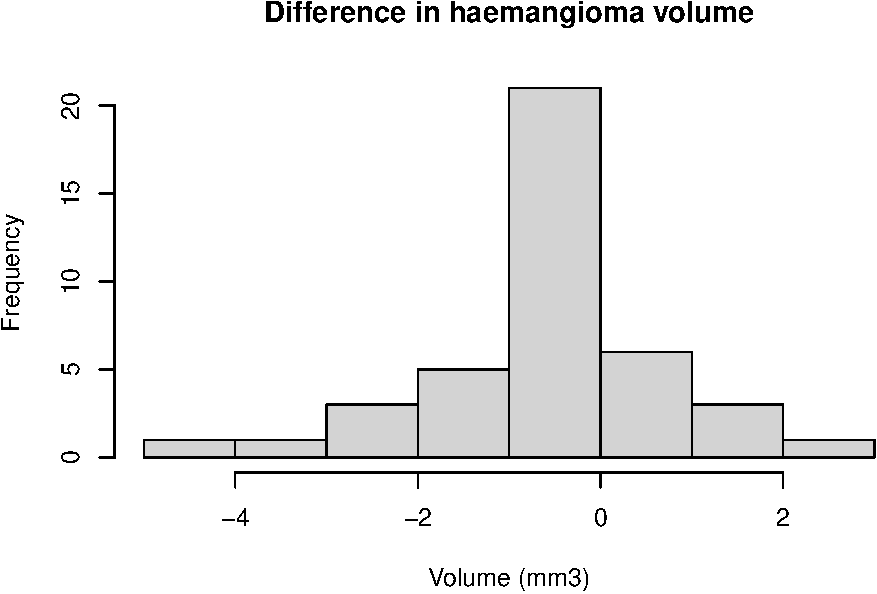
\includegraphics{phcm9795-solutions-R_files/figure-latex/unnamed-chunk-50-1.pdf}

\begin{quote}
As we can see from the histogram, the differences in volume at the beginning and end of the study are reasonably symmetrically distributed. Although the distribution is very peaked, there are no influential outliers and the t-test is robust to the deviation of the normality assumption.
\end{quote}

\begin{quote}
To conduct the paired t-test in R, we use the \texttt{t.test()} function, specifying the two columns of haemangioma volume and \texttt{paired=TRUE}:
\end{quote}

\begin{Shaded}
\begin{Highlighting}[]
\CommentTok{\# Using ttestPS from jmv}
\FunctionTok{ttestPS}\NormalTok{(}\AttributeTok{data=}\NormalTok{babies, }\AttributeTok{pairs=}\FunctionTok{list}\NormalTok{(}\FunctionTok{list}\NormalTok{(}\AttributeTok{i1 =} \StringTok{\textquotesingle{}week\_12\textquotesingle{}}\NormalTok{, }\AttributeTok{i2 =} \StringTok{\textquotesingle{}baseline\textquotesingle{}}\NormalTok{)), }\AttributeTok{meanDiff=}\ConstantTok{TRUE}\NormalTok{, }\AttributeTok{ci=}\ConstantTok{TRUE}\NormalTok{)}
\end{Highlighting}
\end{Shaded}

\begin{verbatim}
## 
##  PAIRED SAMPLES T-TEST
## 
##  Paired Samples T-Test                                                                                                                        
##  ──────────────────────────────────────────────────────────────────────────────────────────────────────────────────────────────────────────── 
##                                          statistic    df          p            Mean difference    SE difference    Lower         Upper        
##  ──────────────────────────────────────────────────────────────────────────────────────────────────────────────────────────────────────────── 
##    week_12    baseline    Student's t    -1.959437    40.00000    0.0570564         -0.4021951        0.2052605    -0.8170422    0.01265192   
##  ────────────────────────────────────────────────────────────────────────────────────────────────────────────────────────────────────────────
\end{verbatim}

The code for the \texttt{ttestPS()} function is quite cumbersome. You may want to use the \texttt{t.test()} function:

\begin{Shaded}
\begin{Highlighting}[]
\CommentTok{\# Using t.test}
\FunctionTok{t.test}\NormalTok{(babies}\SpecialCharTok{$}\NormalTok{week\_12, babies}\SpecialCharTok{$}\NormalTok{baseline, }\AttributeTok{paired=}\ConstantTok{TRUE}\NormalTok{)}
\end{Highlighting}
\end{Shaded}

\begin{verbatim}
## 
##  Paired t-test
## 
## data:  babies$week_12 and babies$baseline
## t = -1.9594, df = 40, p-value = 0.05706
## alternative hypothesis: true mean difference is not equal to 0
## 95 percent confidence interval:
##  -0.81704216  0.01265192
## sample estimates:
## mean difference 
##      -0.4021951
\end{verbatim}

\begin{quote}
The output shows that the mean volume at week 12 of 1.94 mm\textsuperscript{3} was lower than the mean of 2.34 mm\textsuperscript{3} at baseline. The mean decrease is 0.40 mm\textsuperscript{3} (95\% CI −0.01 to 0.82). From the paired t-test results, we can see that t = -1.96 with 40 df and P = 0.057. This P-value provides only weak evidence that the topical medication has an effect on haemangioma volume among children aged 6 months to 2 years. The P-value of 0.057 is consistent with the 95\% CI just crossing the line of no difference (i.e.~0 mm3).
\end{quote}

\begin{quote}
{[}Note that the estimated difference and its confidence interval (-0.40: 95\% CI from -0.82 to 0.01) is presented as if it were an \emph{increase} from baseline to 12-weeks. As the mean difference is negative, we can interpreted the estimates as \emph{reductions} by multiplying each value by -1.{]}
\end{quote}

\begin{enumerate}
\def\labelenumi{\alph{enumi})}
\setcounter{enumi}{2}
\tightlist
\item
  What are the limitations of this study?
\end{enumerate}

\begin{quote}
In a paired design, each subject serves as their own control (here by comparing the change in volume of the haemangioma at baseline and after 12 weeks of treatment). However, the reduction of −0.40 mm3 on average could have been due to the new medication or to the natural history of the condition. A better design would be a randomised controlled trial where subjects are randomised to the new treatment or the usual treatment and compare the volume between the 2 groups. More information on randomised controlled trials and other study designs is given in PHCM9794: Foundations of Epidemiology.
\end{quote}

\hypertarget{module-5-full-script}{%
\chapter*{Module 5: Full script}\label{module-5-full-script}}
\addcontentsline{toc}{chapter}{Module 5: Full script}

\begin{Shaded}
\begin{Highlighting}[]
\CommentTok{\# Author: Timothy Dobbins}
\CommentTok{\# Date: June, 2022}
\CommentTok{\# Purpose: Learning activities for Module 5}

\CommentTok{\# If necessary, install the BSDA package:}
\CommentTok{\# install.packages("BSDA")}
\FunctionTok{library}\NormalTok{(BSDA)}
\FunctionTok{library}\NormalTok{(jmv)}

\CommentTok{\# Activity 5.2}
\CommentTok{\# Calculate difference in means by hand:}
\FloatTok{19.9} \SpecialCharTok{{-}} \FloatTok{13.9}

\CommentTok{\# t{-}test assuming equal variance}
\FunctionTok{tsum.test}\NormalTok{(}\AttributeTok{mean.x=}\FloatTok{19.9}\NormalTok{, }\AttributeTok{s.x=}\FloatTok{5.9}\NormalTok{, }\AttributeTok{n.x=}\DecValTok{12}\NormalTok{,}
          \AttributeTok{mean.y=}\FloatTok{13.9}\NormalTok{, }\AttributeTok{s.y=}\FloatTok{6.2}\NormalTok{, }\AttributeTok{n.y=}\DecValTok{15}\NormalTok{,}
          \AttributeTok{mu=}\DecValTok{0}\NormalTok{, }\AttributeTok{alternative=}\StringTok{"two.sided"}\NormalTok{, }\AttributeTok{var.equal =} \ConstantTok{TRUE}\NormalTok{)}

\CommentTok{\# Activity 5.3}
\NormalTok{anaemia }\OtherTok{\textless{}{-}} \FunctionTok{readRDS}\NormalTok{(}\StringTok{"data/activities/Activity\_S5.3.rds"}\NormalTok{)}

\FunctionTok{descriptives}\NormalTok{(}\AttributeTok{data=}\NormalTok{anaemia, }\AttributeTok{vars=}\NormalTok{hematocrit,}
             \AttributeTok{splitBy =}\NormalTok{ group,}
             \AttributeTok{skew =} \ConstantTok{TRUE}\NormalTok{)}

\CommentTok{\# Plotting by group using the method from Module 2:}
\NormalTok{anaemia\_i }\OtherTok{\textless{}{-}} \FunctionTok{subset}\NormalTok{(anaemia, group}\SpecialCharTok{==}\StringTok{"Intervention"}\NormalTok{)}
\NormalTok{anaemia\_sc }\OtherTok{\textless{}{-}} \FunctionTok{subset}\NormalTok{(anaemia, group}\SpecialCharTok{==}\StringTok{"Standard care"}\NormalTok{)}

\CommentTok{\# Set the graphics parameters to plot 2 rows and 2 columns:}
\FunctionTok{par}\NormalTok{(}\AttributeTok{mfrow=}\FunctionTok{c}\NormalTok{(}\DecValTok{2}\NormalTok{,}\DecValTok{2}\NormalTok{))}

\CommentTok{\# Specify each plot separately}
\FunctionTok{hist}\NormalTok{(anaemia\_i}\SpecialCharTok{$}\NormalTok{hematocrit, }\AttributeTok{xlab=}\StringTok{"Hematocrit"}\NormalTok{, }\AttributeTok{main=}\StringTok{"Intervention"}\NormalTok{)}
\FunctionTok{hist}\NormalTok{(anaemia\_sc}\SpecialCharTok{$}\NormalTok{hematocrit, }\AttributeTok{xlab=}\StringTok{"Hematocrit"}\NormalTok{, }\AttributeTok{main=}\StringTok{"Standard care"}\NormalTok{)}

\FunctionTok{boxplot}\NormalTok{(anaemia\_i}\SpecialCharTok{$}\NormalTok{hematocrit, }\AttributeTok{ylab=}\StringTok{"Hematocrit"}\NormalTok{, }\AttributeTok{main=}\StringTok{"Intervention"}\NormalTok{)}
\FunctionTok{boxplot}\NormalTok{(anaemia\_sc}\SpecialCharTok{$}\NormalTok{hematocrit, }\AttributeTok{ylab=}\StringTok{"Hematocrit"}\NormalTok{, }\AttributeTok{main=}\StringTok{"Standard care"}\NormalTok{)}


\CommentTok{\# Create plots using common axis limits}
\FunctionTok{hist}\NormalTok{(anaemia\_i}\SpecialCharTok{$}\NormalTok{hematocrit, }\AttributeTok{xlab=}\StringTok{"Hematocrit"}\NormalTok{, }\AttributeTok{main=}\StringTok{"Intervention"}\NormalTok{,}
     \AttributeTok{xlim=}\FunctionTok{c}\NormalTok{(}\DecValTok{28}\NormalTok{, }\DecValTok{38}\NormalTok{))}
\FunctionTok{hist}\NormalTok{(anaemia\_sc}\SpecialCharTok{$}\NormalTok{hematocrit, }\AttributeTok{xlab=}\StringTok{"Hematocrit"}\NormalTok{, }\AttributeTok{main=}\StringTok{"Standard care"}\NormalTok{,}
     \AttributeTok{xlim=}\FunctionTok{c}\NormalTok{(}\DecValTok{28}\NormalTok{, }\DecValTok{38}\NormalTok{))}

\FunctionTok{boxplot}\NormalTok{(anaemia\_i}\SpecialCharTok{$}\NormalTok{hematocrit, }\AttributeTok{ylab=}\StringTok{"Hematocrit"}\NormalTok{, }\AttributeTok{main=}\StringTok{"Intervention"}\NormalTok{,}
        \AttributeTok{ylim=}\FunctionTok{c}\NormalTok{(}\DecValTok{28}\NormalTok{, }\DecValTok{38}\NormalTok{))}
\FunctionTok{boxplot}\NormalTok{(anaemia\_sc}\SpecialCharTok{$}\NormalTok{hematocrit, }\AttributeTok{ylab=}\StringTok{"Hematocrit"}\NormalTok{, }\AttributeTok{main=}\StringTok{"Standard care"}\NormalTok{,}
        \AttributeTok{ylim=}\FunctionTok{c}\NormalTok{(}\DecValTok{28}\NormalTok{, }\DecValTok{38}\NormalTok{))}

\CommentTok{\# Reset graphics parameters}
\FunctionTok{par}\NormalTok{(}\AttributeTok{mfrow=}\FunctionTok{c}\NormalTok{(}\DecValTok{1}\NormalTok{,}\DecValTok{1}\NormalTok{))}

\CommentTok{\# Welch\textquotesingle{}s t{-}test}
\FunctionTok{ttestIS}\NormalTok{(}\AttributeTok{data=}\NormalTok{anaemia, }\AttributeTok{vars=}\NormalTok{hematocrit, }\AttributeTok{group=}\NormalTok{group, }\AttributeTok{meanDiff=}\ConstantTok{TRUE}\NormalTok{, }\AttributeTok{ci=}\ConstantTok{TRUE}\NormalTok{, }\AttributeTok{welchs=}\ConstantTok{TRUE}\NormalTok{)}

\CommentTok{\# Activity 5.4}
\NormalTok{babies }\OtherTok{\textless{}{-}} \FunctionTok{readRDS}\NormalTok{(}\StringTok{"data/activities/Activity\_S5.4.rds"}\NormalTok{)}

\NormalTok{babies}\SpecialCharTok{$}\NormalTok{diff }\OtherTok{=}\NormalTok{ babies}\SpecialCharTok{$}\NormalTok{week\_12 }\SpecialCharTok{{-}}\NormalTok{ babies}\SpecialCharTok{$}\NormalTok{baseline}
\FunctionTok{hist}\NormalTok{(babies}\SpecialCharTok{$}\NormalTok{diff, }\AttributeTok{xlab=}\StringTok{"Volume (mm3)"}\NormalTok{, }\AttributeTok{main=}\StringTok{"Difference in haemangioma volume"}\NormalTok{)}

\CommentTok{\# Using ttestPS from jmv}
\FunctionTok{ttestPS}\NormalTok{(}\AttributeTok{data=}\NormalTok{babies, }\AttributeTok{pairs=}\FunctionTok{list}\NormalTok{(}\FunctionTok{list}\NormalTok{(}\AttributeTok{i1 =} \StringTok{\textquotesingle{}week\_12\textquotesingle{}}\NormalTok{, }\AttributeTok{i2 =} \StringTok{\textquotesingle{}baseline\textquotesingle{}}\NormalTok{)), }\AttributeTok{meanDiff=}\ConstantTok{TRUE}\NormalTok{, }\AttributeTok{ci=}\ConstantTok{TRUE}\NormalTok{)}

\CommentTok{\# Using t.test}
\FunctionTok{t.test}\NormalTok{(babies}\SpecialCharTok{$}\NormalTok{week\_12, babies}\SpecialCharTok{$}\NormalTok{baseline, }\AttributeTok{paired=}\ConstantTok{TRUE}\NormalTok{)}
\end{Highlighting}
\end{Shaded}

\hypertarget{module-6-solutions-to-learning-activities}{%
\chapter*{Module 6: Solutions to Learning Activities}\label{module-6-solutions-to-learning-activities}}
\addcontentsline{toc}{chapter}{Module 6: Solutions to Learning Activities}

\hypertarget{activity-6.1}{%
\subsection*{Activity 6.1}\label{activity-6.1}}
\addcontentsline{toc}{subsection}{Activity 6.1}

In a clinical trial involving a dietary intervention, 150 adult volunteers agreed to participate. The investigator wanted to know whether this sample was representative of the general population. One interesting finding was that 90 of the participants drink alcohol regularly compared to 70\% of the general population.

\begin{enumerate}
\def\labelenumi{\alph{enumi})}
\tightlist
\item
  State the null hypothesis
\end{enumerate}

\begin{quote}
Null hypothesis: The proportion of volunteers who consume alcohol regularly is the same as the proportion who consume alcohol regularly in the general population.
\end{quote}

\begin{enumerate}
\def\labelenumi{\alph{enumi})}
\setcounter{enumi}{1}
\tightlist
\item
  Calculate the 95\% CI for the proportion of regular drinkers in the sample using R.
\end{enumerate}

\begin{Shaded}
\begin{Highlighting}[]
\FunctionTok{library}\NormalTok{(DescTools)}

\CommentTok{\# BinomCI from DescTools calculates a Wilson confidence interval:}
\FunctionTok{BinomCI}\NormalTok{(}\DecValTok{90}\NormalTok{, }\AttributeTok{n=}\DecValTok{150}\NormalTok{, }\AttributeTok{method=}\StringTok{"wilson"}\NormalTok{)}
\end{Highlighting}
\end{Shaded}

\begin{verbatim}
##      est    lwr.ci    upr.ci
## [1,] 0.6 0.5200492 0.6749568
\end{verbatim}

\begin{Shaded}
\begin{Highlighting}[]
\CommentTok{\# The default binom.test calculates a Wald confidence interval}
\FunctionTok{binom.test}\NormalTok{(}\DecValTok{90}\NormalTok{, }\AttributeTok{n=}\DecValTok{150}\NormalTok{, }\AttributeTok{p=}\FloatTok{0.7}\NormalTok{)}
\end{Highlighting}
\end{Shaded}

\begin{verbatim}
## 
##  Exact binomial test
## 
## data:  90 and 150
## number of successes = 90, number of trials = 150, p-value = 0.009553
## alternative hypothesis: true probability of success is not equal to 0.7
## 95 percent confidence interval:
##  0.5169313 0.6790370
## sample estimates:
## probability of success 
##                    0.6
\end{verbatim}

\begin{quote}
The proportion of volunteers who drink alcohol regularly is estimated as 60\%, with a 95\% confidence interval from 52\% to 67\%. The 95\% confidence interval can be interpreted as: we are 95\% confident that the true prevalence of alcohol drinkers in the population from where the sample was drawn lies between 52\% and 67\%. Note that the prevalence of regular drinkers in the general population is 70\%, which does not fall within the 95\% CI calculated from the sample. This may be because the participants were not randomly selected from the general population; they volunteered to participate in the study.
\end{quote}

\begin{enumerate}
\def\labelenumi{\alph{enumi})}
\setcounter{enumi}{2}
\tightlist
\item
  Use the R file Activity\_S6.1.rds to decide if the sample of volunteers is representative of the population.
\end{enumerate}

\begin{quote}
We have stated the null hypothesis in part (a):
\end{quote}

\begin{quote}
Null hypothesis: The proportion of volunteers who consume alcohol regularly is the same as the proportion who consume alcohol regularly in the general population.
\end{quote}

\begin{quote}
The one-sample proportion test has been calculated with the \texttt{binom.test} command in (a). If we only had individual data (i.e.~did not have the summary results above), we would need to tabulate the data first:
\end{quote}

\begin{Shaded}
\begin{Highlighting}[]
\NormalTok{alcohol }\OtherTok{\textless{}{-}} \FunctionTok{readRDS}\NormalTok{(}\StringTok{"data/activities/Activity\_S6.1.rds"}\NormalTok{)}
\FunctionTok{table}\NormalTok{(alcohol}\SpecialCharTok{$}\NormalTok{Drinking\_Status)}
\end{Highlighting}
\end{Shaded}

\begin{verbatim}
## 
## Non-drinker     Drinker 
##          60          90
\end{verbatim}

\begin{Shaded}
\begin{Highlighting}[]
\FunctionTok{binom.test}\NormalTok{(}\DecValTok{90}\NormalTok{, }\AttributeTok{n=}\DecValTok{150}\NormalTok{, }\AttributeTok{p=}\FloatTok{0.7}\NormalTok{)}
\end{Highlighting}
\end{Shaded}

\begin{verbatim}
## 
##  Exact binomial test
## 
## data:  90 and 150
## number of successes = 90, number of trials = 150, p-value = 0.009553
## alternative hypothesis: true probability of success is not equal to 0.7
## 95 percent confidence interval:
##  0.5169313 0.6790370
## sample estimates:
## probability of success 
##                    0.6
\end{verbatim}

The R output gives the P-value from a two-sided test of 0.0096. Thus, we can conclude that there is strong evidence that the proportion of drinkers among the sample population of the dietary intervention group (60\%) is lower than that (70\%) in the general population.

\hypertarget{activity-6.2}{%
\subsection*{Activity 6.2}\label{activity-6.2}}
\addcontentsline{toc}{subsection}{Activity 6.2}

A survey was conducted of a random sample of upper primary school children to measure the prevalence of asthma using questionnaires completed by the parents. A total of 514 children were enrolled. Use the R dataset Activity\_S6.2.rds for this activity.

\begin{enumerate}
\def\labelenumi{\alph{enumi})}
\tightlist
\item
  Calculate the relative risk and odds ratio with 95\% confidence interval using Stata for children to have asthma symptoms if they are male? Which risk estimate would be the correct statistic to report?
\end{enumerate}

\begin{quote}
Before we begin analysing any binary data, we must ensure that the binary variables of interest are coded as factors, with the positive exposure and outcomes ordered first. We can check this using the \texttt{summary()} function:
\end{quote}

\begin{Shaded}
\begin{Highlighting}[]
\FunctionTok{library}\NormalTok{(jmv)}
\NormalTok{asthma }\OtherTok{\textless{}{-}} \FunctionTok{readRDS}\NormalTok{(}\StringTok{"data/activities/Activity\_S6.2.rds"}\NormalTok{)}

\FunctionTok{summary}\NormalTok{(asthma}\SpecialCharTok{$}\NormalTok{Asthma)}
\end{Highlighting}
\end{Shaded}

\begin{verbatim}
## Yes  No 
## 119 395
\end{verbatim}

\begin{Shaded}
\begin{Highlighting}[]
\FunctionTok{summary}\NormalTok{(asthma}\SpecialCharTok{$}\NormalTok{Gender)}
\end{Highlighting}
\end{Shaded}

\begin{verbatim}
##   Male Female   NA's 
##    258    242     14
\end{verbatim}

\begin{quote}
Here, Asthma is coded with ``Yes'' as the first level, as required. Gender is coded with ``Male'' as the first level, which means that R will produce summaries of male vs female. Note that there are 14 missing values for gender, indicated as NA.
\end{quote}

\begin{quote}
The relative risk of asthma can be calculated using the \texttt{contTables()} function within the \texttt{jmv} library. The relative risk is calculated using \texttt{relRisk\ =\ TRUE}, and the proportion of asthma within each sex calculated using \texttt{pcRow\ =\ TRUE}:
\end{quote}

\begin{Shaded}
\begin{Highlighting}[]
\FunctionTok{contTables}\NormalTok{(}\AttributeTok{data=}\NormalTok{asthma, }\AttributeTok{rows=}\NormalTok{Gender, }\AttributeTok{cols=}\NormalTok{Asthma,}
          \AttributeTok{pcRow =} \ConstantTok{TRUE}\NormalTok{, }\AttributeTok{relRisk =} \ConstantTok{TRUE}\NormalTok{)}
\end{Highlighting}
\end{Shaded}

\begin{verbatim}
## 
##  CONTINGENCY TABLES
## 
##  Contingency Tables                                                
##  ───────────────────────────────────────────────────────────────── 
##    Gender                    Yes          No           Total       
##  ───────────────────────────────────────────────────────────────── 
##    Male      Observed               70          188          258   
##              % within row     27.13178     72.86822    100.00000   
##                                                                    
##    Female    Observed               46          196          242   
##              % within row     19.00826     80.99174    100.00000   
##                                                                    
##    Total     Observed              116          384          500   
##              % within row     23.20000     76.80000    100.00000   
##  ───────────────────────────────────────────────────────────────── 
## 
## 
##  χ² Tests                              
##  ───────────────────────────────────── 
##          Value       df    p           
##  ───────────────────────────────────── 
##    χ²    4.624920     1    0.0315107   
##    N          500                      
##  ───────────────────────────────────── 
## 
## 
##  Comparative Measures                                    
##  ─────────────────────────────────────────────────────── 
##                     Value         Lower       Upper      
##  ─────────────────────────────────────────────────────── 
##    Relative risk    1.427368 ᵃ    1.028159    1.981579   
##  ─────────────────────────────────────────────────────── 
##    ᵃ Rows compared
\end{verbatim}

\begin{quote}
From the output we can see that the relative risk of Asthma for males compared to females is 1.43 (95\% CI: 1.03 to 1.98).
\end{quote}

\begin{quote}
To calculate the odds ratio, we use \texttt{odds\ =\ TRUE}:
\end{quote}

\begin{Shaded}
\begin{Highlighting}[]
\FunctionTok{contTables}\NormalTok{(}\AttributeTok{data=}\NormalTok{asthma, }\AttributeTok{rows=}\NormalTok{Gender, }\AttributeTok{cols=}\NormalTok{Asthma,}
          \AttributeTok{odds =} \ConstantTok{TRUE}\NormalTok{)}
\end{Highlighting}
\end{Shaded}

\begin{verbatim}
## 
##  CONTINGENCY TABLES
## 
##  Contingency Tables                
##  ───────────────────────────────── 
##    Gender    Yes    No     Total   
##  ───────────────────────────────── 
##    Male       70    188      258   
##    Female     46    196      242   
##    Total     116    384      500   
##  ───────────────────────────────── 
## 
## 
##  χ² Tests                              
##  ───────────────────────────────────── 
##          Value       df    p           
##  ───────────────────────────────────── 
##    χ²    4.624920     1    0.0315107   
##    N          500                      
##  ───────────────────────────────────── 
## 
## 
##  Comparative Measures                               
##  ────────────────────────────────────────────────── 
##                  Value       Lower       Upper      
##  ────────────────────────────────────────────────── 
##    Odds ratio    1.586494    1.039904    2.420381   
##  ──────────────────────────────────────────────────
\end{verbatim}

\begin{quote}
The OR of Asthma 1.59 (95\% CI: 1.04 to 2.42) for males compared to females.
\end{quote}

\begin{quote}
The relative risk is the correct risk estimate to use as this a cross-sectional study. The relative risk is a direct comparison of the proportion with asthma symptoms in each exposure group. The odds ratio is only appropriate for a case-control study.
\end{quote}

\begin{enumerate}
\def\labelenumi{\alph{enumi})}
\setcounter{enumi}{1}
\tightlist
\item
  Use the tabulated data on the frequency of cases and exposure you obtained in R output in part a to calculate RR and OR with their 95\% confidence interval using R.
\end{enumerate}

\begin{quote}
This question assumes we are only given the values of the four cells in the cross-tabulation. We can re-write this table as follows to explain the process of entering summarised data:
\end{quote}

\begin{longtable}[]{@{}ccc@{}}
\toprule()
Gender & Asthma & Number \\
\midrule()
\endhead
Male & Yes & 70 \\
Male & No & 188 \\
Female & Yes & 46 \\
Female & No & 196 \\
\bottomrule()
\end{longtable}

\begin{quote}
We can enter these data in a dataframe, comprising three vectors, as follows:
\end{quote}

\begin{Shaded}
\begin{Highlighting}[]
\NormalTok{asthma\_summary }\OtherTok{\textless{}{-}} \FunctionTok{data.frame}\NormalTok{(}
  \AttributeTok{Gender =} \FunctionTok{c}\NormalTok{(}\StringTok{"Male"}\NormalTok{, }\StringTok{"Male"}\NormalTok{, }\StringTok{"Female"}\NormalTok{, }\StringTok{"Female"}\NormalTok{),}
  \AttributeTok{Asthma =} \FunctionTok{c}\NormalTok{(}\StringTok{"Yes"}\NormalTok{, }\StringTok{"No"}\NormalTok{, }\StringTok{"Yes"}\NormalTok{, }\StringTok{"No"}\NormalTok{),}
  \AttributeTok{Number =} \FunctionTok{c}\NormalTok{(}\DecValTok{70}\NormalTok{, }\DecValTok{188}\NormalTok{, }\DecValTok{46}\NormalTok{, }\DecValTok{196}\NormalTok{))}
\end{Highlighting}
\end{Shaded}

\begin{quote}
We need to define Gender and Asthma as factors. Here we must define the \texttt{levels} \textbf{in the order we want the categories to appear in the table}. Note that as Gender and Asthma are entered as text variables, we can omit \texttt{labels} command when defining the factors, and the factor will be labelled using the text entry:
\end{quote}

\begin{Shaded}
\begin{Highlighting}[]
\NormalTok{asthma\_summary}\SpecialCharTok{$}\NormalTok{Gender }\OtherTok{\textless{}{-}} \FunctionTok{factor}\NormalTok{(asthma\_summary}\SpecialCharTok{$}\NormalTok{Gender,}
                                \AttributeTok{levels =} \FunctionTok{c}\NormalTok{(}\StringTok{"Male"}\NormalTok{, }\StringTok{"Female"}\NormalTok{))}

\NormalTok{asthma\_summary}\SpecialCharTok{$}\NormalTok{Asthma }\OtherTok{\textless{}{-}} \FunctionTok{factor}\NormalTok{(asthma\_summary}\SpecialCharTok{$}\NormalTok{Asthma,}
                                \AttributeTok{levels =} \FunctionTok{c}\NormalTok{(}\StringTok{"Yes"}\NormalTok{, }\StringTok{"No"}\NormalTok{))}
\end{Highlighting}
\end{Shaded}

\begin{quote}
We can calculate the relative risk using the summarised data in the same was done previously. However, we need to include the number of observations in each cell using the \texttt{counts} command:
\end{quote}

\begin{Shaded}
\begin{Highlighting}[]
\FunctionTok{contTables}\NormalTok{(}\AttributeTok{data=}\NormalTok{asthma\_summary,}
           \AttributeTok{rows =}\NormalTok{ Gender, }\AttributeTok{cols =}\NormalTok{ Asthma,}
           \AttributeTok{counts =}\NormalTok{ Number,}
           \AttributeTok{relRisk =} \ConstantTok{TRUE}\NormalTok{)}
\end{Highlighting}
\end{Shaded}

\begin{verbatim}
## 
##  CONTINGENCY TABLES
## 
##  Contingency Tables                
##  ───────────────────────────────── 
##    Gender    Yes    No     Total   
##  ───────────────────────────────── 
##    Male       70    188      258   
##    Female     46    196      242   
##    Total     116    384      500   
##  ───────────────────────────────── 
## 
## 
##  χ² Tests                              
##  ───────────────────────────────────── 
##          Value       df    p           
##  ───────────────────────────────────── 
##    χ²    4.624920     1    0.0315107   
##    N          500                      
##  ───────────────────────────────────── 
## 
## 
##  Comparative Measures                                    
##  ─────────────────────────────────────────────────────── 
##                     Value         Lower       Upper      
##  ─────────────────────────────────────────────────────── 
##    Relative risk    1.427368 ᵃ    1.028159    1.981579   
##  ─────────────────────────────────────────────────────── 
##    ᵃ Rows compared
\end{verbatim}

\begin{quote}
The output from the summarised data is identical to the output of the individual-level data.
\end{quote}

\hypertarget{activity-6.3}{%
\subsection*{Activity 6.3}\label{activity-6.3}}
\addcontentsline{toc}{subsection}{Activity 6.3}

In a study to determine the cause of mortality, 89 people were followed up for 5 years. The participants are classified into two groups of those who did or did not have a heart attack. At the end of the follow-up 15 people died among them 10 had a heart attack. Among the 74 survivors 35 had a heart attack. Present the data on a 2x2 table and calculate relative risk of death from heart attack with 95\% confidence interval using R.

\begin{quote}
The cross-tabulation of heart attack and mortality is given in Table 6.1.
\end{quote}

\begin{longtable}[]{@{}lllc@{}}
\toprule()
HeartAttack & Death & & Total \\
\midrule()
\endhead
& Yes & No & \\
Yes & 10 & 35 & 45 \\
No & 5 & 39 & 44 \\
Total & 15 & 74 & 89 \\
\bottomrule()
\end{longtable}

\begin{quote}
To calculate relative risk using the information from Table 6.1, we enter first enter the summarised data into a new dataframe:
\end{quote}

\begin{Shaded}
\begin{Highlighting}[]
\NormalTok{mortality }\OtherTok{\textless{}{-}} \FunctionTok{data.frame}\NormalTok{(}
  \AttributeTok{HeartAttack =} \FunctionTok{c}\NormalTok{(}\StringTok{"Yes"}\NormalTok{, }\StringTok{"Yes"}\NormalTok{, }\StringTok{"No"}\NormalTok{, }\StringTok{"No"}\NormalTok{),}
  \AttributeTok{Death =} \FunctionTok{c}\NormalTok{(}\StringTok{"Yes"}\NormalTok{, }\StringTok{"No"}\NormalTok{, }\StringTok{"Yes"}\NormalTok{, }\StringTok{"No"}\NormalTok{),}
  \AttributeTok{n =} \FunctionTok{c}\NormalTok{(}\DecValTok{10}\NormalTok{, }\DecValTok{35}\NormalTok{, }\DecValTok{5}\NormalTok{, }\DecValTok{39}\NormalTok{))}

\NormalTok{mortality}\SpecialCharTok{$}\NormalTok{HeartAttack }\OtherTok{\textless{}{-}} \FunctionTok{factor}\NormalTok{(mortality}\SpecialCharTok{$}\NormalTok{HeartAttack,}
                                \AttributeTok{levels =} \FunctionTok{c}\NormalTok{(}\StringTok{"Yes"}\NormalTok{, }\StringTok{"No"}\NormalTok{))}

\NormalTok{mortality}\SpecialCharTok{$}\NormalTok{Death }\OtherTok{\textless{}{-}} \FunctionTok{factor}\NormalTok{(mortality}\SpecialCharTok{$}\NormalTok{Death,}
                                \AttributeTok{levels =} \FunctionTok{c}\NormalTok{(}\StringTok{"Yes"}\NormalTok{, }\StringTok{"No"}\NormalTok{))}
\end{Highlighting}
\end{Shaded}

\begin{quote}
We then estimate the relative risk using the \texttt{contTables()} function:
\end{quote}

\begin{Shaded}
\begin{Highlighting}[]
\FunctionTok{contTables}\NormalTok{(}\AttributeTok{data =}\NormalTok{ mortality,}
           \AttributeTok{rows =}\NormalTok{ HeartAttack, }\AttributeTok{cols =}\NormalTok{ Death,}
           \AttributeTok{counts =}\NormalTok{ n,}
           \AttributeTok{pcRow =} \ConstantTok{TRUE}\NormalTok{, }\AttributeTok{relRisk =} \ConstantTok{TRUE}\NormalTok{)}
\end{Highlighting}
\end{Shaded}

\begin{verbatim}
## 
##  CONTINGENCY TABLES
## 
##  Contingency Tables                                                     
##  ────────────────────────────────────────────────────────────────────── 
##    HeartAttack                    Yes          No           Total       
##  ────────────────────────────────────────────────────────────────────── 
##    Yes            Observed               10           35           45   
##                   % within row     22.22222     77.77778    100.00000   
##                                                                         
##    No             Observed                5           39           44   
##                   % within row     11.36364     88.63636    100.00000   
##                                                                         
##    Total          Observed               15           74           89   
##                   % within row     16.85393     83.14607    100.00000   
##  ────────────────────────────────────────────────────────────────────── 
## 
## 
##  χ² Tests                              
##  ───────────────────────────────────── 
##          Value       df    p           
##  ───────────────────────────────────── 
##    χ²    1.871883     1    0.1712595   
##    N           89                      
##  ───────────────────────────────────── 
## 
## 
##  Comparative Measures                                     
##  ──────────────────────────────────────────────────────── 
##                     Value         Lower        Upper      
##  ──────────────────────────────────────────────────────── 
##    Relative risk    1.955556 ᵃ    0.7267615    5.261971   
##  ──────────────────────────────────────────────────────── 
##    ᵃ Rows compared
\end{verbatim}

From the output we can see that the relative risk of death from heart attack is 1.96 (95\% CI: 0.73 to 5.26).

\hypertarget{activity-6.4}{%
\subsection*{Activity 6.4}\label{activity-6.4}}
\addcontentsline{toc}{subsection}{Activity 6.4}

A study is conducted to test the hypothesis that the observed frequency of a certain health outcome is 30\%. If the results yield a CI around the sample proportion that extends from 23.8 to 30.2, what can you say about the evidence against the null hypothesis?

\begin{quote}
As the 95\% confidence interval includes the hypothesised population proportion, we can infer that the P-value of the study will be greater than 0.05. Hence, this study provides weak to no evidence against the null hypothesis.
\end{quote}

\hypertarget{activity-6.5}{%
\subsection*{Activity 6.5}\label{activity-6.5}}
\addcontentsline{toc}{subsection}{Activity 6.5}

In an experiment to test the effect of vitamin C on IQ scores, the following confidence intervals were estimated around the percentage of people with improved scores for five different populations:

\begin{longtable}[]{@{}ccc@{}}
\toprule()
Population & \% with improved IQ & 95\% confidence interval \\
\midrule()
\endhead
1 & 35.0 & 32.0 to 38.0 \\
2 & 29.5 & 25.0 to 34.0 \\
3 & 43.5 & 42.0 to 45.0 \\
4 & 30.5 & 20.0 to 41.0 \\
5 & 24.5 & 21.0 to 28.0 \\
\bottomrule()
\end{longtable}

\begin{enumerate}
\def\labelenumi{\alph{enumi})}
\tightlist
\item
  Which CI is the most precise?
\end{enumerate}

\begin{quote}
Population 3. This has the smallest interval which is 3 (42 - 45).
\end{quote}

\begin{enumerate}
\def\labelenumi{\alph{enumi})}
\setcounter{enumi}{1}
\tightlist
\item
  Which CI implies the largest sample size?
\end{enumerate}

\begin{quote}
Population 3. The larger the sample size, the smaller the standard error and hence narrower the confidence interval. Therefore the largest sample size will have the narrowest confidence interval provided that the frequency is the same.
\end{quote}

\begin{enumerate}
\def\labelenumi{\alph{enumi})}
\setcounter{enumi}{2}
\item
  Which CI is the least precise?
  \textgreater{} Population 4. This has the widest interval which is 21 (41 - 20), thus is less precise than the others.
\item
  Which CI most strongly supports the conclusion that vitamin C increases IQ score and why?
\end{enumerate}

\begin{quote}
Population 3. This has the narrowest confidence interval where the lower bound is higher than the upper bound of all others.
\end{quote}

\begin{enumerate}
\def\labelenumi{\alph{enumi})}
\setcounter{enumi}{4}
\tightlist
\item
  Which would most likely to stimulate the investigator to conduct an additional experiment using a larger sample size?
\end{enumerate}

\begin{quote}
Population 4. This estimate is the least precise. By increasing sample size, the estimate of frequency as shown by the 95\% CI would become narrower.
\end{quote}

\hypertarget{module-6-full-script}{%
\chapter*{Module 6: Full script}\label{module-6-full-script}}
\addcontentsline{toc}{chapter}{Module 6: Full script}

\begin{Shaded}
\begin{Highlighting}[]
\CommentTok{\# Author: Timothy Dobbins}
\CommentTok{\# Date: June, 2022}
\CommentTok{\# Purpose: Learning activities for Module 6}

\CommentTok{\# Activity 6.1}

\FunctionTok{library}\NormalTok{(DescTools)}

\CommentTok{\# BinomCI from DescTools calculates a Wilson confidence interval:}
\FunctionTok{BinomCI}\NormalTok{(}\DecValTok{90}\NormalTok{, }\AttributeTok{n=}\DecValTok{150}\NormalTok{, }\AttributeTok{method=}\StringTok{"wilson"}\NormalTok{)}

\CommentTok{\# The default binom.test calculates a Wald confidence interval}
\FunctionTok{binom.test}\NormalTok{(}\DecValTok{90}\NormalTok{, }\AttributeTok{n=}\DecValTok{150}\NormalTok{, }\AttributeTok{p=}\FloatTok{0.7}\NormalTok{)}

\NormalTok{alcohol }\OtherTok{\textless{}{-}} \FunctionTok{readRDS}\NormalTok{(}\StringTok{"data/activities/Activity\_S6.1.rds"}\NormalTok{)}
\FunctionTok{table}\NormalTok{(alcohol}\SpecialCharTok{$}\NormalTok{Drinking\_Status)}

\FunctionTok{binom.test}\NormalTok{(}\DecValTok{90}\NormalTok{, }\AttributeTok{n=}\DecValTok{150}\NormalTok{, }\AttributeTok{p=}\FloatTok{0.7}\NormalTok{)}

\CommentTok{\# Activity 6.2}

\FunctionTok{library}\NormalTok{(jmv)}
\NormalTok{asthma }\OtherTok{\textless{}{-}} \FunctionTok{readRDS}\NormalTok{(}\StringTok{"data/activities/Activity\_S6.2.rds"}\NormalTok{)}

\FunctionTok{summary}\NormalTok{(asthma}\SpecialCharTok{$}\NormalTok{Asthma)}
\FunctionTok{summary}\NormalTok{(asthma}\SpecialCharTok{$}\NormalTok{Gender)}

\FunctionTok{contTables}\NormalTok{(}\AttributeTok{data=}\NormalTok{asthma, }\AttributeTok{rows=}\NormalTok{Gender, }\AttributeTok{cols=}\NormalTok{Asthma,}
          \AttributeTok{pcRow =} \ConstantTok{TRUE}\NormalTok{, }\AttributeTok{relRisk =} \ConstantTok{TRUE}\NormalTok{)}

\FunctionTok{contTables}\NormalTok{(}\AttributeTok{data=}\NormalTok{asthma, }\AttributeTok{rows=}\NormalTok{Gender, }\AttributeTok{cols=}\NormalTok{Asthma,}
          \AttributeTok{odds =} \ConstantTok{TRUE}\NormalTok{)}

\NormalTok{asthma\_summary }\OtherTok{\textless{}{-}} \FunctionTok{data.frame}\NormalTok{(}
  \AttributeTok{Gender =} \FunctionTok{c}\NormalTok{(}\StringTok{"Male"}\NormalTok{, }\StringTok{"Male"}\NormalTok{, }\StringTok{"Female"}\NormalTok{, }\StringTok{"Female"}\NormalTok{),}
  \AttributeTok{Asthma =} \FunctionTok{c}\NormalTok{(}\StringTok{"Yes"}\NormalTok{, }\StringTok{"No"}\NormalTok{, }\StringTok{"Yes"}\NormalTok{, }\StringTok{"No"}\NormalTok{),}
  \AttributeTok{Number =} \FunctionTok{c}\NormalTok{(}\DecValTok{70}\NormalTok{, }\DecValTok{188}\NormalTok{, }\DecValTok{46}\NormalTok{, }\DecValTok{196}\NormalTok{))}

\NormalTok{asthma\_summary}\SpecialCharTok{$}\NormalTok{Gender }\OtherTok{\textless{}{-}} \FunctionTok{factor}\NormalTok{(asthma\_summary}\SpecialCharTok{$}\NormalTok{Gender,}
                                \AttributeTok{levels =} \FunctionTok{c}\NormalTok{(}\StringTok{"Male"}\NormalTok{, }\StringTok{"Female"}\NormalTok{))}

\NormalTok{asthma\_summary}\SpecialCharTok{$}\NormalTok{Asthma }\OtherTok{\textless{}{-}} \FunctionTok{factor}\NormalTok{(asthma\_summary}\SpecialCharTok{$}\NormalTok{Asthma,}
                                \AttributeTok{levels =} \FunctionTok{c}\NormalTok{(}\StringTok{"Yes"}\NormalTok{, }\StringTok{"No"}\NormalTok{))}

\FunctionTok{contTables}\NormalTok{(}\AttributeTok{data=}\NormalTok{asthma\_summary,}
           \AttributeTok{rows =}\NormalTok{ Gender, }\AttributeTok{cols =}\NormalTok{ Asthma,}
           \AttributeTok{counts =}\NormalTok{ Number,}
           \AttributeTok{relRisk =} \ConstantTok{TRUE}\NormalTok{)}


\CommentTok{\# Activity 6.3}
\NormalTok{mortality }\OtherTok{\textless{}{-}} \FunctionTok{data.frame}\NormalTok{(}
  \AttributeTok{HeartAttack =} \FunctionTok{c}\NormalTok{(}\StringTok{"Yes"}\NormalTok{, }\StringTok{"Yes"}\NormalTok{, }\StringTok{"No"}\NormalTok{, }\StringTok{"No"}\NormalTok{),}
  \AttributeTok{Death =} \FunctionTok{c}\NormalTok{(}\StringTok{"Yes"}\NormalTok{, }\StringTok{"No"}\NormalTok{, }\StringTok{"Yes"}\NormalTok{, }\StringTok{"No"}\NormalTok{),}
  \AttributeTok{n =} \FunctionTok{c}\NormalTok{(}\DecValTok{10}\NormalTok{, }\DecValTok{35}\NormalTok{, }\DecValTok{5}\NormalTok{, }\DecValTok{39}\NormalTok{))}

\NormalTok{mortality}\SpecialCharTok{$}\NormalTok{HeartAttack }\OtherTok{\textless{}{-}} \FunctionTok{factor}\NormalTok{(mortality}\SpecialCharTok{$}\NormalTok{HeartAttack,}
                                \AttributeTok{levels =} \FunctionTok{c}\NormalTok{(}\StringTok{"Yes"}\NormalTok{, }\StringTok{"No"}\NormalTok{))}

\NormalTok{mortality}\SpecialCharTok{$}\NormalTok{Death }\OtherTok{\textless{}{-}} \FunctionTok{factor}\NormalTok{(mortality}\SpecialCharTok{$}\NormalTok{Death,}
                                \AttributeTok{levels =} \FunctionTok{c}\NormalTok{(}\StringTok{"Yes"}\NormalTok{, }\StringTok{"No"}\NormalTok{))}

\FunctionTok{contTables}\NormalTok{(}\AttributeTok{data =}\NormalTok{ mortality,}
           \AttributeTok{rows =}\NormalTok{ HeartAttack, }\AttributeTok{cols =}\NormalTok{ Death,}
           \AttributeTok{counts =}\NormalTok{ n,}
           \AttributeTok{pcRow =} \ConstantTok{TRUE}\NormalTok{, }\AttributeTok{relRisk =} \ConstantTok{TRUE}\NormalTok{)}
\end{Highlighting}
\end{Shaded}

\hypertarget{module-7-solutions-to-learning-activities}{%
\chapter*{Module 7: Solutions to Learning Activities}\label{module-7-solutions-to-learning-activities}}
\addcontentsline{toc}{chapter}{Module 7: Solutions to Learning Activities}

\hypertarget{activity-7.1}{%
\subsection*{Activity 7.1}\label{activity-7.1}}
\addcontentsline{toc}{subsection}{Activity 7.1}

Use the file Activity\_S7.1.rds to further investigate whether there is a gender difference in asthma in a random sample of 514 upper primary school children:

\begin{enumerate}
\def\labelenumi{\alph{enumi})}
\tightlist
\item
  Use a contingency table (cross-tabulation) to determine the observed and expected frequencies. Which cell has the lowest expected cell count?
\end{enumerate}

\begin{quote}
Here we can use the \texttt{contTables()} function within \texttt{jmv} with the option \texttt{exp\ =\ TRUE} to present the expected frequencies.
\end{quote}

\begin{Shaded}
\begin{Highlighting}[]
\FunctionTok{library}\NormalTok{(jmv)}

\NormalTok{children }\OtherTok{\textless{}{-}} \FunctionTok{readRDS}\NormalTok{(}\StringTok{"data/activities/Activity\_S7.1.rds"}\NormalTok{)}

\FunctionTok{contTables}\NormalTok{(}\AttributeTok{data=}\NormalTok{children, }\AttributeTok{rows =}\NormalTok{ gender, }\AttributeTok{cols =}\NormalTok{ asthma,}
           \AttributeTok{exp =} \ConstantTok{TRUE}\NormalTok{)}
\end{Highlighting}
\end{Shaded}

\begin{verbatim}
## 
##  CONTINGENCY TABLES
## 
##  Contingency Tables                                          
##  ─────────────────────────────────────────────────────────── 
##    gender                No          Yes          Total      
##  ─────────────────────────────────────────────────────────── 
##    Female    Observed         196           46         242   
##              Expected    185.8560     56.14400    242.0000   
##                                                              
##    Male      Observed         188           70         258   
##              Expected    198.1440     59.85600    258.0000   
##                                                              
##    Total     Observed         384          116         500   
##              Expected    384.0000    116.00000    500.0000   
##  ─────────────────────────────────────────────────────────── 
## 
## 
##  χ² Tests                              
##  ───────────────────────────────────── 
##          Value       df    p           
##  ───────────────────────────────────── 
##    χ²    4.624920     1    0.0315107   
##    N          500                      
##  ─────────────────────────────────────
\end{verbatim}

\begin{quote}
In the table, cell ``b'' (asthma symptoms among females) gives the lowest expected frequency which is 56.1 - much larger than 5. Therefore, we can conduct a Pearson's chi-square test.
\end{quote}

\begin{enumerate}
\def\labelenumi{\alph{enumi})}
\setcounter{enumi}{1}
\tightlist
\item
  Use a chi-squared test to evaluate the hypothesis and interpret the result. Are the assumptions for a chi-squared test met? Calculate the 95\% CI of the difference in proportions.
\end{enumerate}

\begin{quote}
Note the table above has asthma symptoms with the ``No'' level appearing first. To estimate the difference in the proportion with asthma symptoms, we should re-order the \texttt{asthma} factor so that ``Yes'' appears first.
\end{quote}

\begin{Shaded}
\begin{Highlighting}[]
\FunctionTok{str}\NormalTok{(children}\SpecialCharTok{$}\NormalTok{asthma)}
\end{Highlighting}
\end{Shaded}

\begin{verbatim}
##  Factor w/ 2 levels "No","Yes": 2 1 1 2 1 1 2 2 2 1 ...
##  - attr(*, "label")= chr "Asthma symptoms"
\end{verbatim}

\begin{Shaded}
\begin{Highlighting}[]
\NormalTok{children}\SpecialCharTok{$}\NormalTok{asthma }\OtherTok{\textless{}{-}} \FunctionTok{relevel}\NormalTok{(children}\SpecialCharTok{$}\NormalTok{asthma, }\AttributeTok{ref=}\StringTok{"Yes"}\NormalTok{)}

\FunctionTok{str}\NormalTok{(children}\SpecialCharTok{$}\NormalTok{asthma)}
\end{Highlighting}
\end{Shaded}

\begin{verbatim}
##  Factor w/ 2 levels "Yes","No": 1 2 2 1 2 2 1 1 1 2 ...
\end{verbatim}

\begin{quote}
We can now request a contingency table with row-percents using \texttt{pcRow\ =\ TRUE} and \texttt{diffProp} to request the difference in proportions.
\end{quote}

\begin{Shaded}
\begin{Highlighting}[]
\FunctionTok{contTables}\NormalTok{(}\AttributeTok{data=}\NormalTok{children, }\AttributeTok{rows =}\NormalTok{ gender, }\AttributeTok{cols =}\NormalTok{ asthma,}
           \AttributeTok{pcRow =} \ConstantTok{TRUE}\NormalTok{, }\AttributeTok{diffProp =} \ConstantTok{TRUE}\NormalTok{)}
\end{Highlighting}
\end{Shaded}

\begin{verbatim}
## 
##  CONTINGENCY TABLES
## 
##  Contingency Tables                                                
##  ───────────────────────────────────────────────────────────────── 
##    gender                    Yes          No           Total       
##  ───────────────────────────────────────────────────────────────── 
##    Female    Observed               46          196          242   
##              % within row     19.00826     80.99174    100.00000   
##                                                                    
##    Male      Observed               70          188          258   
##              % within row     27.13178     72.86822    100.00000   
##                                                                    
##    Total     Observed              116          384          500   
##              % within row     23.20000     76.80000    100.00000   
##  ───────────────────────────────────────────────────────────────── 
## 
## 
##  χ² Tests                              
##  ───────────────────────────────────── 
##          Value       df    p           
##  ───────────────────────────────────── 
##    χ²    4.624920     1    0.0315107   
##    N          500                      
##  ───────────────────────────────────── 
## 
## 
##  Comparative Measures                                                           
##  ────────────────────────────────────────────────────────────────────────────── 
##                                   Value            Lower         Upper          
##  ────────────────────────────────────────────────────────────────────────────── 
##    Difference in 2 proportions    -0.08123518 ᵃ    -0.1546347    -0.007835685   
##  ────────────────────────────────────────────────────────────────────────────── 
##    ᵃ Rows compared
\end{verbatim}

\begin{quote}
The P value is 0.032 from the Chi-Square value of 4.62 with 1 df, which provides evidence of a difference in the proportions diagnosed with asthma between males and females.
\end{quote}

\begin{quote}
There are four assumptions for a Pearson's chi-squared test:
\end{quote}

\begin{quote}
\begin{itemize}
\tightlist
\item
  each observation must be independent
\item
  each participant is represented in the table once only
\item
  at least 80\% of the expected cell counts should exceed a value of five
\item
  all expected cell counts should exceed a value of one.
\end{itemize}
\end{quote}

\begin{quote}
It is evident from the study design that the observations are independent, and each participant was presented in the table once only (asthma was measured once only). Therefore, the first two assumptions are met. From part (a), we can see that smallest expected cell count is 56.1 (\textgreater5). Thus, the last two assumptions are also met.
\end{quote}

\begin{quote}
The proportion of asthma is 27.1\% among males and 19.0\% among females. There is evidence of a difference in the proportions diagnosed with asthma between males and females (chi-square=4.62 with 1 df, P=0.03). The proportion with asthma is 8.0\% lower in females than males with a 95\% confidence interval of 0.8\% to 15.5\% (read from the Risk difference).
\end{quote}

\hypertarget{activity-7.2}{%
\subsection*{Activity 7.2}\label{activity-7.2}}
\addcontentsline{toc}{subsection}{Activity 7.2}

The file Activity\_S7.2.rds summarises the 5-year mortality data for 89 people who did or did not have a heart attack.

\begin{enumerate}
\def\labelenumi{\alph{enumi})}
\tightlist
\item
  State the null hypothesis.
\end{enumerate}

\begin{quote}
Null hypothesis: There is no association between having a heart attack and risk of death in the next five years
\end{quote}

\begin{enumerate}
\def\labelenumi{\alph{enumi})}
\setcounter{enumi}{1}
\tightlist
\item
  Using R, carry out the appropriate significance test to evaluate the hypothesis. Do the data fulfil the assumptions of the statistical test you have used?
\end{enumerate}

\begin{quote}
A Pearson's Chi-Square test is appropriate to test the null hypothesis. To check whether our data fulfils the assumptions for a Pearson's Chi-Squared test we need to obtain the expected frequencies for the 2 × 2 table using cross-tabulation:
\end{quote}

\begin{Shaded}
\begin{Highlighting}[]
\NormalTok{heart }\OtherTok{\textless{}{-}} \FunctionTok{readRDS}\NormalTok{(}\StringTok{"data/activities/Activity\_S7.2.rds"}\NormalTok{)}

\FunctionTok{head}\NormalTok{(heart)}
\end{Highlighting}
\end{Shaded}

\begin{verbatim}
##   survival heart_attack mort
## 1       No          yes  yes
## 2       No          yes  yes
## 3       No          yes  yes
## 4       No          yes  yes
## 5       No          yes  yes
## 6       No          yes  yes
\end{verbatim}

\begin{Shaded}
\begin{Highlighting}[]
\FunctionTok{str}\NormalTok{(heart)}
\end{Highlighting}
\end{Shaded}

\begin{verbatim}
## 'data.frame':    89 obs. of  3 variables:
##  $ survival    : Factor w/ 2 levels "No","yes": 1 1 1 1 1 1 1 1 1 1 ...
##   ..- attr(*, "label")= chr "Survival"
##  $ heart_attack: Factor w/ 2 levels "No","yes": 2 2 2 2 2 2 2 2 2 2 ...
##   ..- attr(*, "label")= chr "Heart_attack"
##  $ mort        : Factor w/ 2 levels "No","yes": 2 2 2 2 2 2 2 2 2 2 ...
##   ..- attr(*, "label")= chr "Death"
\end{verbatim}

\begin{quote}
We can see that each variable has been entered as a factor, but ``No'' is the first level. We should reorder our exposure (\texttt{heart\_attack}) and outcome (\texttt{mort}) so that ``yes'' becomes the first level:
\end{quote}

\begin{Shaded}
\begin{Highlighting}[]
\NormalTok{heart}\SpecialCharTok{$}\NormalTok{heart\_attack }\OtherTok{\textless{}{-}} \FunctionTok{relevel}\NormalTok{(heart}\SpecialCharTok{$}\NormalTok{heart\_attack, }\AttributeTok{ref=}\StringTok{"yes"}\NormalTok{)}
\NormalTok{heart}\SpecialCharTok{$}\NormalTok{mort }\OtherTok{\textless{}{-}} \FunctionTok{relevel}\NormalTok{(heart}\SpecialCharTok{$}\NormalTok{mort, }\AttributeTok{ref=}\StringTok{"yes"}\NormalTok{)}

\FunctionTok{str}\NormalTok{(heart)}
\end{Highlighting}
\end{Shaded}

\begin{verbatim}
## 'data.frame':    89 obs. of  3 variables:
##  $ survival    : Factor w/ 2 levels "No","yes": 1 1 1 1 1 1 1 1 1 1 ...
##   ..- attr(*, "label")= chr "Survival"
##  $ heart_attack: Factor w/ 2 levels "yes","No": 1 1 1 1 1 1 1 1 1 1 ...
##  $ mort        : Factor w/ 2 levels "yes","No": 1 1 1 1 1 1 1 1 1 1 ...
\end{verbatim}

\begin{quote}
We can now use \texttt{contTables()} to produce the 2-by-2 table with expected values:
\end{quote}

\begin{Shaded}
\begin{Highlighting}[]
\FunctionTok{contTables}\NormalTok{(}\AttributeTok{data=}\NormalTok{heart, }\AttributeTok{rows=}\NormalTok{heart\_attack, }\AttributeTok{cols=}\NormalTok{mort,}
           \AttributeTok{exp=}\ConstantTok{TRUE}\NormalTok{)}
\end{Highlighting}
\end{Shaded}

\begin{verbatim}
## 
##  CONTINGENCY TABLES
## 
##  Contingency Tables                                                
##  ───────────────────────────────────────────────────────────────── 
##    heart_attack                yes          No          Total      
##  ───────────────────────────────────────────────────────────────── 
##    yes             Observed           10          35          45   
##                    Expected     7.584270    37.41573    45.00000   
##                                                                    
##    No              Observed            5          39          44   
##                    Expected     7.415730    36.58427    44.00000   
##                                                                    
##    Total           Observed           15          74          89   
##                    Expected    15.000000    74.00000    89.00000   
##  ───────────────────────────────────────────────────────────────── 
## 
## 
##  χ² Tests                              
##  ───────────────────────────────────── 
##          Value       df    p           
##  ───────────────────────────────────── 
##    χ²    1.871883     1    0.1712595   
##    N           89                      
##  ─────────────────────────────────────
\end{verbatim}

\begin{quote}
From the study design, it is clear that the observations are independent, and participants are represented only once in the table. Therefore, the data fulfils the first two assumptions of independence. From the above table we can see that the lowest expected frequency is 7.4, which is greater than 5. Thus, the last two assumptions are also met, and we can use the results from the Pearson's Chi-Squared test.
\end{quote}

\begin{quote}
The P-value from the Chi-Square test (chi-square = 1.87 with 1 df) test statistic is 0.17, that is, there is no evidence of an association between heart attack and mortality during the next 5 years.
\end{quote}

\begin{enumerate}
\def\labelenumi{\alph{enumi})}
\setcounter{enumi}{2}
\tightlist
\item
  Estimate the appropriate risk estimate for mortality. Are the confidence intervals of the risk estimates consistent with the P value?
\end{enumerate}

\begin{quote}
Because this is a follow-up study from where we can estimate incidence, the relative risk is the appropriate risk estimate:
\end{quote}

\begin{Shaded}
\begin{Highlighting}[]
\FunctionTok{contTables}\NormalTok{(}\AttributeTok{data=}\NormalTok{heart, }\AttributeTok{rows=}\NormalTok{heart\_attack, }\AttributeTok{cols=}\NormalTok{mort,}
           \AttributeTok{pcRow =} \ConstantTok{TRUE}\NormalTok{, }\AttributeTok{relRisk =} \ConstantTok{TRUE}\NormalTok{)}
\end{Highlighting}
\end{Shaded}

\begin{verbatim}
## 
##  CONTINGENCY TABLES
## 
##  Contingency Tables                                                      
##  ─────────────────────────────────────────────────────────────────────── 
##    heart_attack                    yes          No           Total       
##  ─────────────────────────────────────────────────────────────────────── 
##    yes             Observed               10           35           45   
##                    % within row     22.22222     77.77778    100.00000   
##                                                                          
##    No              Observed                5           39           44   
##                    % within row     11.36364     88.63636    100.00000   
##                                                                          
##    Total           Observed               15           74           89   
##                    % within row     16.85393     83.14607    100.00000   
##  ─────────────────────────────────────────────────────────────────────── 
## 
## 
##  χ² Tests                              
##  ───────────────────────────────────── 
##          Value       df    p           
##  ───────────────────────────────────── 
##    χ²    1.871883     1    0.1712595   
##    N           89                      
##  ───────────────────────────────────── 
## 
## 
##  Comparative Measures                                     
##  ──────────────────────────────────────────────────────── 
##                     Value         Lower        Upper      
##  ──────────────────────────────────────────────────────── 
##    Relative risk    1.955556 ᵃ    0.7267615    5.261971   
##  ──────────────────────────────────────────────────────── 
##    ᵃ Rows compared
\end{verbatim}

\begin{quote}
The relative risk is 1.96 (95\% CI: 0.73, 5.26). The confidence interval includes the null value (1) which is consistent with the P-value (P = 0.17).
\end{quote}

\begin{quote}
Note that the risk difference would also be an acceptable measure for this study.
\end{quote}

\begin{enumerate}
\def\labelenumi{\alph{enumi})}
\setcounter{enumi}{3}
\tightlist
\item
  Summarise your results and state your conclusion.
\end{enumerate}

\begin{quote}
There is no evidence of an association between heart attack and 5-year mortality (chi-square=1.87 with 1 df, P = 0.17). The risk of dying during next 5 years for those who experienced a heart attack is 1.96 (95\% CI: 0.73, 5.26) times that for those who did not experience a heart attack, but the 95\% confidence interval indicates that the relative risk may be as low as 0.73 and as high as 5.26 (with 95\% confidence).
\end{quote}

\hypertarget{activity-7.3}{%
\subsection*{Activity 7.3}\label{activity-7.3}}
\addcontentsline{toc}{subsection}{Activity 7.3}

The effect of two penicillin allergens B and G was tested in a random sample of 500 people. All people were tested with both allergens. For each person, data were recorded for whether or not there was an allergic reaction to the allergen.

Use the data set Activity\_S7.3.rds to test the null hypothesis that the proportion of participants who react to allergen G is the same as the proportion who react to allergen B. Are the 95\% CI around the difference consistent with the P value?

\begin{quote}
As usual, after reading the data, we should check the ordering of the factor levels for the two variables.
\end{quote}

\begin{Shaded}
\begin{Highlighting}[]
\NormalTok{study }\OtherTok{\textless{}{-}} \FunctionTok{readRDS}\NormalTok{(}\StringTok{"data/activities/Activity\_S7.3.rds"}\NormalTok{)}

\FunctionTok{head}\NormalTok{(study)}
\end{Highlighting}
\end{Shaded}

\begin{verbatim}
##   React_Allergen_G React_Allergen_B
## 1            React            React
## 2            React            React
## 3            React            React
## 4            React            React
## 5            React            React
## 6            React            React
\end{verbatim}

\begin{Shaded}
\begin{Highlighting}[]
\FunctionTok{str}\NormalTok{(study)}
\end{Highlighting}
\end{Shaded}

\begin{verbatim}
## 'data.frame':    500 obs. of  2 variables:
##  $ React_Allergen_G: Factor w/ 2 levels "Don't react",..: 2 2 2 2 2 2 2 2 2 2 ...
##   ..- attr(*, "label")= chr "Reacts to allergen G"
##  $ React_Allergen_B: Factor w/ 2 levels "Don't react",..: 2 2 2 2 2 2 2 2 2 2 ...
##   ..- attr(*, "label")= chr "Reacts to allergen B"
\end{verbatim}

\begin{quote}
It's a little difficult to determine the order from this output, so let's look at a table:
\end{quote}

\begin{Shaded}
\begin{Highlighting}[]
\FunctionTok{table}\NormalTok{(study}\SpecialCharTok{$}\NormalTok{React\_Allergen\_B)}
\end{Highlighting}
\end{Shaded}

\begin{verbatim}
## 
## Don't react       React 
##         432          68
\end{verbatim}

\begin{Shaded}
\begin{Highlighting}[]
\FunctionTok{table}\NormalTok{(study}\SpecialCharTok{$}\NormalTok{React\_Allergen\_G)}
\end{Highlighting}
\end{Shaded}

\begin{verbatim}
## 
## Don't react       React 
##         448          52
\end{verbatim}

\begin{quote}
In both cases, ``Don't react'' is the first level. This should be re-ordered:
\end{quote}

\begin{Shaded}
\begin{Highlighting}[]
\NormalTok{study}\SpecialCharTok{$}\NormalTok{React\_Allergen\_B }\OtherTok{\textless{}{-}} \FunctionTok{relevel}\NormalTok{(study}\SpecialCharTok{$}\NormalTok{React\_Allergen\_B, }\AttributeTok{ref=}\StringTok{"React"}\NormalTok{)}
\NormalTok{study}\SpecialCharTok{$}\NormalTok{React\_Allergen\_G }\OtherTok{\textless{}{-}} \FunctionTok{relevel}\NormalTok{(study}\SpecialCharTok{$}\NormalTok{React\_Allergen\_G, }\AttributeTok{ref=}\StringTok{"React"}\NormalTok{)}
\end{Highlighting}
\end{Shaded}

\begin{quote}
Because the data are paired, McNemar's test should be used to test the null hypothesis using the \texttt{contTablesPaired()} function:
\end{quote}

\begin{Shaded}
\begin{Highlighting}[]
\FunctionTok{contTablesPaired}\NormalTok{(}\AttributeTok{data=}\NormalTok{study,}
                 \AttributeTok{rows=}\NormalTok{React\_Allergen\_B,}
                 \AttributeTok{cols=}\NormalTok{React\_Allergen\_G)}
\end{Highlighting}
\end{Shaded}

\begin{verbatim}
## 
##  PAIRED SAMPLES CONTINGENCY TABLES
## 
##  Contingency Tables                                    
##  ───────────────────────────────────────────────────── 
##    React_Allergen_B    React    Don't react    Total   
##  ───────────────────────────────────────────────────── 
##    React                  40             28       68   
##    Don't react            12            420      432   
##    Total                  52            448      500   
##  ───────────────────────────────────────────────────── 
## 
## 
##  McNemar Test                          
##  ───────────────────────────────────── 
##          Value       df    p           
##  ───────────────────────────────────── 
##    χ²    6.400000     1    0.0114120   
##    N          500                      
##  ─────────────────────────────────────
\end{verbatim}

\begin{quote}
We use the \texttt{mcNemarDiff()} function (stored in Microsoft Teams and \href{https://gist.githubusercontent.com/timothydobbins/525d25271b04b2ea72aae70c4aac8b01/raw/6b69f5b229d50daeac4c2f4cf4331e88b0c65717/mcNemarDiff.R}{here}) to estimate the proportions, the difference in proportions and its 95\% confidence interval. We should copy the function and paste it into R. Note that when defining the variables to be summarised, the variable names must be surrounded by quotation marks.
\end{quote}

\begin{Shaded}
\begin{Highlighting}[]
\DocumentationTok{\#\#\# Copied from Microsoft Teams}
\NormalTok{mcNemarDiff }\OtherTok{\textless{}{-}} \ControlFlowTok{function}\NormalTok{(data, var1, var2, }\AttributeTok{digits =} \DecValTok{3}\NormalTok{) \{}
  \ControlFlowTok{if}\NormalTok{ (}\SpecialCharTok{!}\FunctionTok{requireNamespace}\NormalTok{(}\StringTok{"epibasix"}\NormalTok{, }\AttributeTok{quietly =} \ConstantTok{TRUE}\NormalTok{)) \{}
    \FunctionTok{stop}\NormalTok{(}\StringTok{"This function requires epibasix to be installed"}\NormalTok{)}
\NormalTok{  \}}
  
\NormalTok{  tab }\OtherTok{\textless{}{-}} \FunctionTok{table}\NormalTok{(data[[var1]], data[[var2]])}
\NormalTok{  p1 }\OtherTok{\textless{}{-}}\NormalTok{ (tab[}\DecValTok{1}\NormalTok{, }\DecValTok{1}\NormalTok{] }\SpecialCharTok{+}\NormalTok{ tab[}\DecValTok{1}\NormalTok{, }\DecValTok{2}\NormalTok{]) }\SpecialCharTok{/} \FunctionTok{sum}\NormalTok{(tab)}
\NormalTok{  p2 }\OtherTok{\textless{}{-}}\NormalTok{ (tab[}\DecValTok{1}\NormalTok{, }\DecValTok{1}\NormalTok{] }\SpecialCharTok{+}\NormalTok{ tab[}\DecValTok{2}\NormalTok{, }\DecValTok{1}\NormalTok{]) }\SpecialCharTok{/} \FunctionTok{sum}\NormalTok{(tab)}
\NormalTok{  pd }\OtherTok{\textless{}{-}}\NormalTok{ epibasix}\SpecialCharTok{::}\FunctionTok{mcNemar}\NormalTok{(tab)}\SpecialCharTok{$}\NormalTok{rd}
\NormalTok{  pd.cil }\OtherTok{\textless{}{-}}\NormalTok{ epibasix}\SpecialCharTok{::}\FunctionTok{mcNemar}\NormalTok{(tab)}\SpecialCharTok{$}\NormalTok{rd.CIL}
\NormalTok{  pd.ciu }\OtherTok{\textless{}{-}}\NormalTok{ epibasix}\SpecialCharTok{::}\FunctionTok{mcNemar}\NormalTok{(tab)}\SpecialCharTok{$}\NormalTok{rd.CIU}
  \FunctionTok{print}\NormalTok{(}\FunctionTok{paste0}\NormalTok{(}
    \StringTok{"Proportion 1: "}\NormalTok{,}
    \FunctionTok{format}\NormalTok{(}\FunctionTok{round}\NormalTok{(p1, }\AttributeTok{digits =}\NormalTok{ digits), }\AttributeTok{nsmall =}\NormalTok{ digits),}
    \StringTok{"; Proportion 2: "}\NormalTok{, }\FunctionTok{format}\NormalTok{(}\FunctionTok{round}\NormalTok{(p2, }\AttributeTok{digits =}\NormalTok{ digits), }\AttributeTok{nsmall =}\NormalTok{ digits)}
\NormalTok{  ))}
  \FunctionTok{print}\NormalTok{(}\FunctionTok{paste0}\NormalTok{(}
    \StringTok{"Difference in paired proportions: "}\NormalTok{,}
    \FunctionTok{format}\NormalTok{(}\FunctionTok{round}\NormalTok{(pd, }\AttributeTok{digits =}\NormalTok{ digits), }\AttributeTok{nsmall =}\NormalTok{ digits),}
    \StringTok{"; 95\% CI: "}\NormalTok{, }\FunctionTok{format}\NormalTok{(}\FunctionTok{round}\NormalTok{(pd.cil, }\AttributeTok{digits =}\NormalTok{ digits), }\AttributeTok{nsmall =}\NormalTok{ digits),}
    \StringTok{" to "}\NormalTok{, }\FunctionTok{format}\NormalTok{(}\FunctionTok{round}\NormalTok{(pd.ciu, }\AttributeTok{digits =}\NormalTok{ digits), }\AttributeTok{nsmall =}\NormalTok{ digits)}
\NormalTok{  ))}
\NormalTok{\}}
\DocumentationTok{\#\#\# End copy}

\FunctionTok{mcNemarDiff}\NormalTok{(}\AttributeTok{data =}\NormalTok{ study, }\AttributeTok{var1 =} \StringTok{"React\_Allergen\_B"}\NormalTok{, }\AttributeTok{var2 =} \StringTok{"React\_Allergen\_G"}\NormalTok{, }\AttributeTok{digits =} \DecValTok{3}\NormalTok{)}
\end{Highlighting}
\end{Shaded}

\begin{verbatim}
## [1] "Proportion 1: 0.136; Proportion 2: 0.104"
## [1] "Difference in paired proportions: 0.032; 95% CI: 0.005 to 0.059"
\end{verbatim}

\begin{quote}
The McNemar's test result shows evidence of a difference in reactions to allergens B and G (chi-square=6.40 with 1 df, P = 0.011).
\end{quote}

\begin{quote}
The output from the \texttt{mcNemarDiff()} function shows that 13.6\% of participants react to allergen B and 10.4\% of participants react to allergen G, with the difference in reaction rate of 3.2\% (95\% CI: 0.5\% to 5.9\%). The 95\% CI does not include the null value (which is 0), which is consistent with the P-value being less than 0.05 (P = 0.011).
\end{quote}

\begin{quote}
Therefore, we can conclude that there is evidence (chi-square=6.40 with 1 df, P = 0.011) of a difference in the effect of penicillin allergen B and G. A total of 3.2\% more patients reacted to penicillin B (13.6\%) compared to penicillin G (10.4\%), and we are 95\% confident that the true difference in the underlying population is between 0.5\% and 5.9\%.
\end{quote}

\hypertarget{activity-7.4}{%
\subsection*{Activity 7.4}\label{activity-7.4}}
\addcontentsline{toc}{subsection}{Activity 7.4}

We examined a survey of 200 live births in an urban region in which 2 babies were born prematurely. We also surveyed 80 live births in a rural region and found that 5 babies were born prematurely. Conduct an appropriate statistical analysis to find out whether the proportion of premature births is higher in the rural region.

\begin{quote}
Two cross-sectional surveys were conducted in two different regions (urban and rural), thus the data are independent and each participant appeared in the dataset only once. We need to check the expected frequencies in a 2x2 table to determine if a Pearson's chi-square test or a Fisher's exact test is appropriate.
\end{quote}

\begin{quote}
The data are aggregate, so we need to enter them into R. To produce the required information for the 2x2 table, we need to calculate total number of normal births in each survey by subtracting the number of premature births from the total births. Thus, in the urban area there are 200 − 2 = 198 normal births and in the rural area there are 80 -- 5 = 75 normal births. The data should be entered in the following way:
\end{quote}

\begin{Shaded}
\begin{Highlighting}[]
\NormalTok{babies }\OtherTok{\textless{}{-}} \FunctionTok{data.frame}\NormalTok{(}
  \AttributeTok{region =} \FunctionTok{c}\NormalTok{(}\StringTok{"Urban"}\NormalTok{, }\StringTok{"Urban"}\NormalTok{, }\StringTok{"Rural"}\NormalTok{, }\StringTok{"Rural"}\NormalTok{),}
  \AttributeTok{birth =} \FunctionTok{c}\NormalTok{(}\StringTok{"Premature"}\NormalTok{, }\StringTok{"Not premature"}\NormalTok{, }\StringTok{"Premature"}\NormalTok{, }\StringTok{"Not premature"}\NormalTok{),}
  \AttributeTok{n =} \FunctionTok{c}\NormalTok{(}\DecValTok{2}\NormalTok{, }\DecValTok{198}\NormalTok{, }\DecValTok{5}\NormalTok{, }\DecValTok{75}\NormalTok{)}
\NormalTok{)}

\NormalTok{babies}\SpecialCharTok{$}\NormalTok{region }\OtherTok{\textless{}{-}} \FunctionTok{factor}\NormalTok{(babies}\SpecialCharTok{$}\NormalTok{region, }\AttributeTok{levels=}\FunctionTok{c}\NormalTok{(}\StringTok{"Urban"}\NormalTok{, }\StringTok{"Rural"}\NormalTok{))}
\NormalTok{babies}\SpecialCharTok{$}\NormalTok{birth }\OtherTok{\textless{}{-}} \FunctionTok{factor}\NormalTok{(babies}\SpecialCharTok{$}\NormalTok{birth, }\AttributeTok{levels=}\FunctionTok{c}\NormalTok{(}\StringTok{"Premature"}\NormalTok{, }\StringTok{"Not premature"}\NormalTok{))}

\NormalTok{babies}
\end{Highlighting}
\end{Shaded}

\begin{verbatim}
##   region         birth   n
## 1  Urban     Premature   2
## 2  Urban Not premature 198
## 3  Rural     Premature   5
## 4  Rural Not premature  75
\end{verbatim}

\begin{quote}
We can use \texttt{contTables()} to calculate the expected counts in each cell. As we are using aggregate data, we must use \texttt{counts\ =\ n} to specify that the column \texttt{n} contains the counts.
\end{quote}

\begin{Shaded}
\begin{Highlighting}[]
\FunctionTok{contTables}\NormalTok{(}\AttributeTok{data=}\NormalTok{babies,}
           \AttributeTok{rows =}\NormalTok{ region, }\AttributeTok{cols =}\NormalTok{ birth, }\AttributeTok{counts =}\NormalTok{ n,}
           \AttributeTok{exp =} \ConstantTok{TRUE}\NormalTok{)}
\end{Highlighting}
\end{Shaded}

\begin{verbatim}
## 
##  CONTINGENCY TABLES
## 
##  Contingency Tables                                                
##  ───────────────────────────────────────────────────────────────── 
##    region                Premature    Not premature    Total       
##  ───────────────────────────────────────────────────────────────── 
##    Urban     Observed            2              198          200   
##              Expected     5.000000        195.00000    200.00000   
##                                                                    
##    Rural     Observed            5               75           80   
##              Expected     2.000000         78.00000     80.00000   
##                                                                    
##    Total     Observed            7              273          280   
##              Expected     7.000000        273.00000    280.00000   
##  ───────────────────────────────────────────────────────────────── 
## 
## 
##  χ² Tests                              
##  ───────────────────────────────────── 
##          Value       df    p           
##  ───────────────────────────────────── 
##    χ²    6.461538     1    0.0110234   
##    N          280                      
##  ─────────────────────────────────────
\end{verbatim}

\begin{quote}
We can see from the above output that the lowest expected frequency in cell ``c'' (expected number of premature birth in the urban region) is 2, which is less than 5. Thus, a Pearson's chi-square test is not appropriate and we should conduct Fisher's exact test. For doing this test, we should specify \texttt{fisher\ =\ TRUE}. Output from the test is shown below:
\end{quote}

\begin{Shaded}
\begin{Highlighting}[]
\FunctionTok{contTables}\NormalTok{(}\AttributeTok{data=}\NormalTok{babies,}
           \AttributeTok{rows =}\NormalTok{ region, }\AttributeTok{cols =}\NormalTok{ birth, }\AttributeTok{counts =}\NormalTok{ n,}
           \AttributeTok{pcRow =} \ConstantTok{TRUE}\NormalTok{, }\AttributeTok{exp =} \ConstantTok{TRUE}\NormalTok{, }\AttributeTok{fisher =} \ConstantTok{TRUE}\NormalTok{)}
\end{Highlighting}
\end{Shaded}

\begin{verbatim}
## 
##  CONTINGENCY TABLES
## 
##  Contingency Tables                                                    
##  ───────────────────────────────────────────────────────────────────── 
##    region                    Premature    Not premature    Total       
##  ───────────────────────────────────────────────────────────────────── 
##    Urban     Observed                2              198          200   
##              Expected         5.000000        195.00000    200.00000   
##              % within row      1.00000         99.00000    100.00000   
##                                                                        
##    Rural     Observed                5               75           80   
##              Expected         2.000000         78.00000     80.00000   
##              % within row      6.25000         93.75000    100.00000   
##                                                                        
##    Total     Observed                7              273          280   
##              Expected         7.000000        273.00000    280.00000   
##              % within row      2.50000         97.50000    100.00000   
##  ───────────────────────────────────────────────────────────────────── 
## 
## 
##  χ² Tests                                               
##  ────────────────────────────────────────────────────── 
##                           Value       df    p           
##  ────────────────────────────────────────────────────── 
##    χ²                     6.461538     1    0.0110234   
##    Fisher's exact test                      0.0218217   
##    N                           280                      
##  ──────────────────────────────────────────────────────
\end{verbatim}

\begin{quote}
Here we see the proportion of premature birth in the urban area is only 1\% and in the rural area it is 6\%. The P-value from Fisher's exact test is 0.022. Thus, we can conclude that there is evidence that the proportion of premature birth in the rural area is higher than that in the urban area.
\end{quote}

\hypertarget{module-7-full-script}{%
\chapter*{Module 7: Full script}\label{module-7-full-script}}
\addcontentsline{toc}{chapter}{Module 7: Full script}

\begin{Shaded}
\begin{Highlighting}[]
\CommentTok{\# Author: Timothy Dobbins}
\CommentTok{\# Date: July, 2022}
\CommentTok{\# Purpose: Learning activities for Module 7}

\CommentTok{\# Activity 7.1}

\FunctionTok{library}\NormalTok{(jmv)}

\NormalTok{children }\OtherTok{\textless{}{-}} \FunctionTok{readRDS}\NormalTok{(}\StringTok{"data/activities/Activity\_S7.1.rds"}\NormalTok{)}

\FunctionTok{contTables}\NormalTok{(}\AttributeTok{data=}\NormalTok{children, }\AttributeTok{rows =}\NormalTok{ gender, }\AttributeTok{cols =}\NormalTok{ asthma,}
           \AttributeTok{exp =} \ConstantTok{TRUE}\NormalTok{)}

\CommentTok{\# Check levels of outcome variable}
\FunctionTok{str}\NormalTok{(children}\SpecialCharTok{$}\NormalTok{asthma)}
\NormalTok{children}\SpecialCharTok{$}\NormalTok{asthma }\OtherTok{\textless{}{-}} \FunctionTok{relevel}\NormalTok{(children}\SpecialCharTok{$}\NormalTok{asthma, }\AttributeTok{ref=}\StringTok{"Yes"}\NormalTok{)}
\FunctionTok{str}\NormalTok{(children}\SpecialCharTok{$}\NormalTok{asthma)}

\FunctionTok{contTables}\NormalTok{(}\AttributeTok{data=}\NormalTok{children, }\AttributeTok{rows =}\NormalTok{ gender, }\AttributeTok{cols =}\NormalTok{ asthma,}
           \AttributeTok{pcRow =} \ConstantTok{TRUE}\NormalTok{, }\AttributeTok{diffProp =} \ConstantTok{TRUE}\NormalTok{)}


\CommentTok{\# Activity 7.2}
\NormalTok{heart }\OtherTok{\textless{}{-}} \FunctionTok{readRDS}\NormalTok{(}\StringTok{"data/activities/Activity\_S7.2.rds"}\NormalTok{)}

\FunctionTok{head}\NormalTok{(heart)}
\FunctionTok{str}\NormalTok{(heart)}

\NormalTok{heart}\SpecialCharTok{$}\NormalTok{heart\_attack }\OtherTok{\textless{}{-}} \FunctionTok{relevel}\NormalTok{(heart}\SpecialCharTok{$}\NormalTok{heart\_attack, }\AttributeTok{ref=}\StringTok{"yes"}\NormalTok{)}
\NormalTok{heart}\SpecialCharTok{$}\NormalTok{mort }\OtherTok{\textless{}{-}} \FunctionTok{relevel}\NormalTok{(heart}\SpecialCharTok{$}\NormalTok{mort, }\AttributeTok{ref=}\StringTok{"yes"}\NormalTok{)}
\FunctionTok{str}\NormalTok{(heart)}

\FunctionTok{contTables}\NormalTok{(}\AttributeTok{data=}\NormalTok{heart, }\AttributeTok{rows=}\NormalTok{heart\_attack, }\AttributeTok{cols=}\NormalTok{mort,}
           \AttributeTok{exp=}\ConstantTok{TRUE}\NormalTok{)}

\FunctionTok{contTables}\NormalTok{(}\AttributeTok{data=}\NormalTok{heart, }\AttributeTok{rows=}\NormalTok{heart\_attack, }\AttributeTok{cols=}\NormalTok{mort,}
           \AttributeTok{pcRow =} \ConstantTok{TRUE}\NormalTok{, }\AttributeTok{relRisk =} \ConstantTok{TRUE}\NormalTok{)}


\CommentTok{\# Activity 7.3}
\NormalTok{study }\OtherTok{\textless{}{-}} \FunctionTok{readRDS}\NormalTok{(}\StringTok{"data/activities/Activity\_S7.3.rds"}\NormalTok{)}

\FunctionTok{head}\NormalTok{(study)}
\FunctionTok{str}\NormalTok{(study)}

\FunctionTok{table}\NormalTok{(study}\SpecialCharTok{$}\NormalTok{React\_Allergen\_B)}
\FunctionTok{table}\NormalTok{(study}\SpecialCharTok{$}\NormalTok{React\_Allergen\_G)}

\NormalTok{study}\SpecialCharTok{$}\NormalTok{React\_Allergen\_B }\OtherTok{\textless{}{-}} \FunctionTok{relevel}\NormalTok{(study}\SpecialCharTok{$}\NormalTok{React\_Allergen\_B, }\AttributeTok{ref=}\StringTok{"React"}\NormalTok{)}
\NormalTok{study}\SpecialCharTok{$}\NormalTok{React\_Allergen\_G }\OtherTok{\textless{}{-}} \FunctionTok{relevel}\NormalTok{(study}\SpecialCharTok{$}\NormalTok{React\_Allergen\_G, }\AttributeTok{ref=}\StringTok{"React"}\NormalTok{)}

\FunctionTok{contTablesPaired}\NormalTok{(}\AttributeTok{data=}\NormalTok{study,}
                 \AttributeTok{rows=}\NormalTok{React\_Allergen\_B,}
                 \AttributeTok{cols=}\NormalTok{React\_Allergen\_G)}

\DocumentationTok{\#\#\# Copied from Microsoft Teams}
\NormalTok{mcNemarDiff }\OtherTok{\textless{}{-}} \ControlFlowTok{function}\NormalTok{(data, var1, var2, }\AttributeTok{digits =} \DecValTok{3}\NormalTok{) \{}
  \ControlFlowTok{if}\NormalTok{ (}\SpecialCharTok{!}\FunctionTok{requireNamespace}\NormalTok{(}\StringTok{"epibasix"}\NormalTok{, }\AttributeTok{quietly =} \ConstantTok{TRUE}\NormalTok{)) \{}
    \FunctionTok{stop}\NormalTok{(}\StringTok{"This function requires epibasix to be installed"}\NormalTok{)}
\NormalTok{  \}}
  
\NormalTok{  tab }\OtherTok{\textless{}{-}} \FunctionTok{table}\NormalTok{(data[[var1]], data[[var2]])}
\NormalTok{  p1 }\OtherTok{\textless{}{-}}\NormalTok{ (tab[}\DecValTok{1}\NormalTok{, }\DecValTok{1}\NormalTok{] }\SpecialCharTok{+}\NormalTok{ tab[}\DecValTok{1}\NormalTok{, }\DecValTok{2}\NormalTok{]) }\SpecialCharTok{/} \FunctionTok{sum}\NormalTok{(tab)}
\NormalTok{  p2 }\OtherTok{\textless{}{-}}\NormalTok{ (tab[}\DecValTok{1}\NormalTok{, }\DecValTok{1}\NormalTok{] }\SpecialCharTok{+}\NormalTok{ tab[}\DecValTok{2}\NormalTok{, }\DecValTok{1}\NormalTok{]) }\SpecialCharTok{/} \FunctionTok{sum}\NormalTok{(tab)}
\NormalTok{  pd }\OtherTok{\textless{}{-}}\NormalTok{ epibasix}\SpecialCharTok{::}\FunctionTok{mcNemar}\NormalTok{(tab)}\SpecialCharTok{$}\NormalTok{rd}
\NormalTok{  pd.cil }\OtherTok{\textless{}{-}}\NormalTok{ epibasix}\SpecialCharTok{::}\FunctionTok{mcNemar}\NormalTok{(tab)}\SpecialCharTok{$}\NormalTok{rd.CIL}
\NormalTok{  pd.ciu }\OtherTok{\textless{}{-}}\NormalTok{ epibasix}\SpecialCharTok{::}\FunctionTok{mcNemar}\NormalTok{(tab)}\SpecialCharTok{$}\NormalTok{rd.CIU}
  \FunctionTok{print}\NormalTok{(}\FunctionTok{paste0}\NormalTok{(}
    \StringTok{"Proportion 1: "}\NormalTok{,}
    \FunctionTok{format}\NormalTok{(}\FunctionTok{round}\NormalTok{(p1, }\AttributeTok{digits =}\NormalTok{ digits), }\AttributeTok{nsmall =}\NormalTok{ digits),}
    \StringTok{"; Proportion 2: "}\NormalTok{, }\FunctionTok{format}\NormalTok{(}\FunctionTok{round}\NormalTok{(p2, }\AttributeTok{digits =}\NormalTok{ digits), }\AttributeTok{nsmall =}\NormalTok{ digits)}
\NormalTok{  ))}
  \FunctionTok{print}\NormalTok{(}\FunctionTok{paste0}\NormalTok{(}
    \StringTok{"Difference in paired proportions: "}\NormalTok{,}
    \FunctionTok{format}\NormalTok{(}\FunctionTok{round}\NormalTok{(pd, }\AttributeTok{digits =}\NormalTok{ digits), }\AttributeTok{nsmall =}\NormalTok{ digits),}
    \StringTok{"; 95\% CI: "}\NormalTok{, }\FunctionTok{format}\NormalTok{(}\FunctionTok{round}\NormalTok{(pd.cil, }\AttributeTok{digits =}\NormalTok{ digits), }\AttributeTok{nsmall =}\NormalTok{ digits),}
    \StringTok{" to "}\NormalTok{, }\FunctionTok{format}\NormalTok{(}\FunctionTok{round}\NormalTok{(pd.ciu, }\AttributeTok{digits =}\NormalTok{ digits), }\AttributeTok{nsmall =}\NormalTok{ digits)}
\NormalTok{  ))}
\NormalTok{\}}
\DocumentationTok{\#\#\# End copy}

\FunctionTok{mcNemarDiff}\NormalTok{(}\AttributeTok{data =}\NormalTok{ study, }\AttributeTok{var1 =} \StringTok{"React\_Allergen\_B"}\NormalTok{, }\AttributeTok{var2 =} \StringTok{"React\_Allergen\_G"}\NormalTok{, }\AttributeTok{digits =} \DecValTok{3}\NormalTok{)}


\CommentTok{\# Activity 7.4}
\NormalTok{babies }\OtherTok{\textless{}{-}} \FunctionTok{data.frame}\NormalTok{(}
  \AttributeTok{region =} \FunctionTok{c}\NormalTok{(}\StringTok{"Urban"}\NormalTok{, }\StringTok{"Urban"}\NormalTok{, }\StringTok{"Rural"}\NormalTok{, }\StringTok{"Rural"}\NormalTok{),}
  \AttributeTok{birth =} \FunctionTok{c}\NormalTok{(}\StringTok{"Premature"}\NormalTok{, }\StringTok{"Not premature"}\NormalTok{, }\StringTok{"Premature"}\NormalTok{, }\StringTok{"Not premature"}\NormalTok{),}
  \AttributeTok{n =} \FunctionTok{c}\NormalTok{(}\DecValTok{2}\NormalTok{, }\DecValTok{198}\NormalTok{, }\DecValTok{5}\NormalTok{, }\DecValTok{75}\NormalTok{)}
\NormalTok{)}

\NormalTok{babies}\SpecialCharTok{$}\NormalTok{region }\OtherTok{\textless{}{-}} \FunctionTok{factor}\NormalTok{(babies}\SpecialCharTok{$}\NormalTok{region, }\AttributeTok{levels=}\FunctionTok{c}\NormalTok{(}\StringTok{"Urban"}\NormalTok{, }\StringTok{"Rural"}\NormalTok{))}
\NormalTok{babies}\SpecialCharTok{$}\NormalTok{birth }\OtherTok{\textless{}{-}} \FunctionTok{factor}\NormalTok{(babies}\SpecialCharTok{$}\NormalTok{birth, }\AttributeTok{levels=}\FunctionTok{c}\NormalTok{(}\StringTok{"Premature"}\NormalTok{, }\StringTok{"Not premature"}\NormalTok{))}

\NormalTok{babies}

\FunctionTok{contTables}\NormalTok{(}\AttributeTok{data=}\NormalTok{babies,}
           \AttributeTok{rows =}\NormalTok{ region, }\AttributeTok{cols =}\NormalTok{ birth, }\AttributeTok{counts =}\NormalTok{ n,}
           \AttributeTok{exp =} \ConstantTok{TRUE}\NormalTok{)}

\FunctionTok{contTables}\NormalTok{(}\AttributeTok{data=}\NormalTok{babies,}
           \AttributeTok{rows =}\NormalTok{ region, }\AttributeTok{cols =}\NormalTok{ birth, }\AttributeTok{counts =}\NormalTok{ n,}
           \AttributeTok{pcRow =} \ConstantTok{TRUE}\NormalTok{, }\AttributeTok{exp =} \ConstantTok{TRUE}\NormalTok{, }\AttributeTok{fisher =} \ConstantTok{TRUE}\NormalTok{)}
\end{Highlighting}
\end{Shaded}

\hypertarget{module-8-solutions-to-learning-activities}{%
\chapter*{Module 8: Solutions to Learning Activities}\label{module-8-solutions-to-learning-activities}}
\addcontentsline{toc}{chapter}{Module 8: Solutions to Learning Activities}

\hypertarget{activity-8.1}{%
\subsection*{Activity 8.1}\label{activity-8.1}}
\addcontentsline{toc}{subsection}{Activity 8.1}

To investigate the effect of body weight (kg) on blood plasma volume (mL), data were collected from 30 participants and a simple linear regression analysis was conducted. The slope of the regression was 68 (95\% confidence interval 52 to 84) and the intercept was −1570 (95\% confidence interval −2655 to −492).

\begin{enumerate}
\def\labelenumi{\alph{enumi})}
\tightlist
\item
  What is the outcome variable and explanatory (exposure) variable?
\end{enumerate}

\begin{quote}
Because we want to know the extent to which body weight predicts blood plasma volume, weight is the explanatory variable and blood plasma volume is the outcome.
\end{quote}

\begin{enumerate}
\def\labelenumi{\alph{enumi})}
\setcounter{enumi}{1}
\tightlist
\item
  Interpret the regression slope and its 95\% CI
\end{enumerate}

\begin{quote}
The regression slope is 68 which means that for every 1 kg increase in body weight, blood plasma volume is predicted to increase by 68 mL. The 95\% confidence interval indicates that we are 95\% confident that the true increase in blood plasma volume per 1 kg in body weight lies between 52 mL and 84 mL.
\end{quote}

\begin{enumerate}
\def\labelenumi{\alph{enumi})}
\setcounter{enumi}{2}
\tightlist
\item
  Write the regression equation
\end{enumerate}

\begin{quote}
The estimated regression equation is: Blood plasma volume (mL) = − 1570 + 68 × Body weight (kg)
\end{quote}

\begin{enumerate}
\def\labelenumi{\alph{enumi})}
\setcounter{enumi}{3}
\tightlist
\item
  If we randomly sampled a person from the population and found that their weight is 80kg, what would be the predicted value of plasma volume for this person?
\end{enumerate}

\begin{quote}
By substituting the value of 80 kg into the above equation we can predict that the person's blood plasma level will be: Blood plasma volume = − 1570 + (68 × 80) = 3870 mL.
\end{quote}

\begin{quote}
Therefore, the predicted plasma volume of a person who is 80 kg is 3870 mL.
\end{quote}

\hypertarget{activity-8.2}{%
\subsection*{Activity 8.2}\label{activity-8.2}}
\addcontentsline{toc}{subsection}{Activity 8.2}

To examine whether age predicts IQ, data were collected on 104 people. Use the data in the Stata file Activity\_8.2.dta to answer the following questions.

\begin{enumerate}
\def\labelenumi{\alph{enumi})}
\tightlist
\item
  What are the outcome variable and the explanatory variable?
\end{enumerate}

\begin{quote}
We are examining whether age predicts IQ, not the other way around. Therefore, age is the explanatory variable and IQ is the outcome variable.
\end{quote}

\begin{enumerate}
\def\labelenumi{\alph{enumi})}
\setcounter{enumi}{1}
\tightlist
\item
  Create a scatter plot with the two variables. What can you infer from the scatter plot?
\end{enumerate}

\begin{quote}
The plot shows that as age increases, IQ decreases. In other words, there is a negative relationship between the two variables. The relationship appears roughly linear, but is not strong (the points are quite scattered around the line of best fit).
\end{quote}

\textbf{Figure 1: Scatter plot of IQ against age (years)}

\begin{Shaded}
\begin{Highlighting}[]
\NormalTok{iq }\OtherTok{\textless{}{-}} \FunctionTok{readRDS}\NormalTok{(}\StringTok{"data/activities/Activity\_S8.2.rds"}\NormalTok{)}

\FunctionTok{plot}\NormalTok{(iq}\SpecialCharTok{$}\NormalTok{age, iq}\SpecialCharTok{$}\NormalTok{iq, }
     \AttributeTok{main=}\StringTok{"Scatter plot of IQ against age"}\NormalTok{,}
     \AttributeTok{xlab =} \StringTok{"Age (years)"}\NormalTok{,}
     \AttributeTok{ylab =} \StringTok{"IQ"}\NormalTok{)}

\FunctionTok{abline}\NormalTok{(}\FunctionTok{lm}\NormalTok{(iq}\SpecialCharTok{$}\NormalTok{iq }\SpecialCharTok{\textasciitilde{}}\NormalTok{ iq}\SpecialCharTok{$}\NormalTok{age))}
\end{Highlighting}
\end{Shaded}

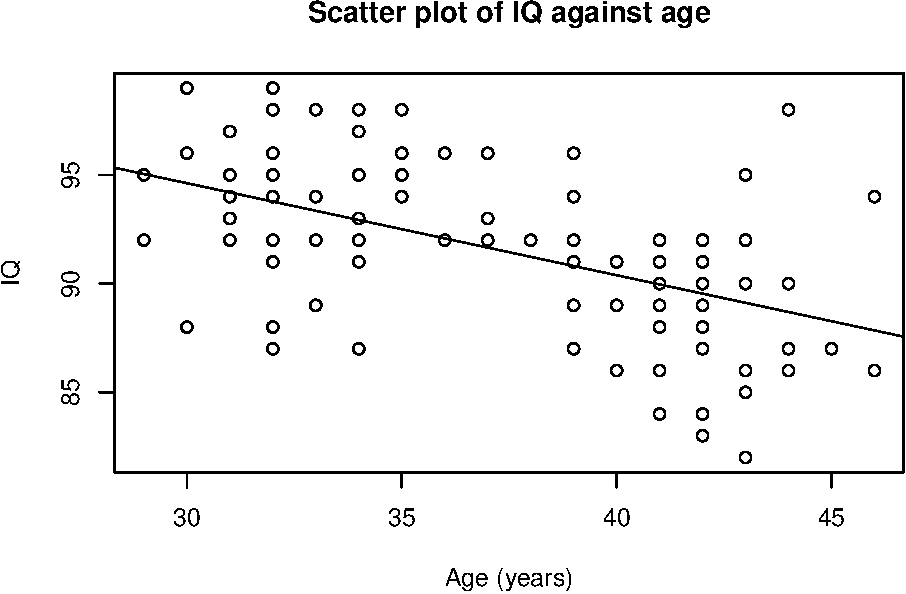
\includegraphics{phcm9795-solutions-R_files/figure-latex/unnamed-chunk-81-1.pdf}

\begin{enumerate}
\def\labelenumi{\alph{enumi})}
\setcounter{enumi}{2}
\tightlist
\item
  Using R, obtain the correlation coefficient between age and IQ and interpret it.
\end{enumerate}

\begin{quote}
To obtain the correlation coefficient, we use the \texttt{cor.test()} function:
\end{quote}

\textbf{R Output 1: Correlation coefficient between IQ and age}

\begin{Shaded}
\begin{Highlighting}[]
\FunctionTok{cor.test}\NormalTok{(iq}\SpecialCharTok{$}\NormalTok{age, iq}\SpecialCharTok{$}\NormalTok{iq)}
\end{Highlighting}
\end{Shaded}

\begin{verbatim}
## 
##  Pearson's product-moment correlation
## 
## data:  iq$age and iq$iq
## t = -6.2429, df = 102, p-value = 9.952e-09
## alternative hypothesis: true correlation is not equal to 0
## 95 percent confidence interval:
##  -0.6523298 -0.3707534
## sample estimates:
##        cor 
## -0.5257982
\end{verbatim}

\begin{quote}
The correlation coefficient is −0.526 indicating that as age increases, IQ decreases, which is consistent with the scatter plot. The P value is \textless0.0001, indicating that there is very strong evidence of a negative linear association between IQ and age, and the strength of that relationship is fair (based on the descriptions given in Section 8.2.1 of the course notes).
\end{quote}

\begin{enumerate}
\def\labelenumi{\alph{enumi})}
\setcounter{enumi}{3}
\tightlist
\item
  Conduct a simple linear regression using R and report the relationship between the two variables including the interpretation of the R-squared value. Are the assumptions for linear regression met in this model?
\end{enumerate}

\begin{quote}
We use the \texttt{lm()} function to regress \texttt{iq} (as the outcome variable) on \texttt{age} (the explanatory variable). To obtain more descriptive output, we save the model as an object, called \texttt{model} here, and then use the \texttt{summary()} function. Finally, confidence intervals for the intercept and slopes are obtained using the \texttt{confint()} function.
\end{quote}

\textbf{R Output 2: Simple linear regression of IQ on Age}

\begin{Shaded}
\begin{Highlighting}[]
\NormalTok{model }\OtherTok{\textless{}{-}} \FunctionTok{lm}\NormalTok{(iq}\SpecialCharTok{$}\NormalTok{iq }\SpecialCharTok{\textasciitilde{}}\NormalTok{ iq}\SpecialCharTok{$}\NormalTok{age)}
\FunctionTok{summary}\NormalTok{(model)}
\end{Highlighting}
\end{Shaded}

\begin{verbatim}
## 
## Call:
## lm(formula = iq$iq ~ iq$age)
## 
## Residuals:
##     Min      1Q  Median      3Q     Max 
## -7.1164 -1.9364  0.2843  2.0367  9.3070 
## 
## Coefficients:
##              Estimate Std. Error t value Pr(>|t|)    
## (Intercept) 107.32431    2.57770  41.636  < 2e-16 ***
## iq$age       -0.42344    0.06783  -6.243 9.95e-09 ***
## ---
## Signif. codes:  0 '***' 0.001 '**' 0.01 '*' 0.05 '.' 0.1 ' ' 1
## 
## Residual standard error: 3.255 on 102 degrees of freedom
## Multiple R-squared:  0.2765, Adjusted R-squared:  0.2694 
## F-statistic: 38.97 on 1 and 102 DF,  p-value: 9.952e-09
\end{verbatim}

\begin{Shaded}
\begin{Highlighting}[]
\FunctionTok{confint}\NormalTok{(model)}
\end{Highlighting}
\end{Shaded}

\begin{verbatim}
##                   2.5 %      97.5 %
## (Intercept) 102.2114610 112.4371606
## iq$age       -0.5579735  -0.2889048
\end{verbatim}

\begin{quote}
The Model Summary table shows the R-squared value of 0.2765. This indicates that 27.6\% of the variation in IQ in the sample can be explained by variability in age.
\end{quote}

\begin{quote}
The coefficients section provides the regression coefficients: an estimated intercept of 107.324 and an estimated slope of -0.423.
\end{quote}

\begin{quote}
The equation is estimated as: IQ = 107 + (−0.423 × age)
\end{quote}

\begin{quote}
(Note: the constant and slope have both been rounded to three significant figures as the outcome and explanatory variables are both measured to two significant figures).
\end{quote}

\begin{quote}
The assumptions for simple linear regression are:
\end{quote}

\begin{quote}
\begin{enumerate}
\def\labelenumi{\arabic{enumi}.}
\tightlist
\item
  the observations are independent of one another;
\item
  the relation between the explanatory variable and the outcome variable is linear;
\item
  the residuals are normally distributed.
\end{enumerate}
\end{quote}

\begin{quote}
Information on the first assumption come from the study design. It is not mentioned in the study description that the data were collected on more than one occasion from each participant or that the participants are related to one another in any ways. Therefore, the observations are independent of one another.
\end{quote}

\begin{quote}
Evidence on the second assumption of a linear relationship between the outcome and explanatory variables is obtained from the scatterplot. Figure 1 demonstrates a linear relationship between age and IQ and so this assumption is also satisfied.
\end{quote}

\begin{quote}
To check the third assumption, that the residuals are normally distributed, we need to first generate and save the residuals in a new object. In R, we can save the residuals using the \texttt{resid()} function:
\end{quote}

\begin{Shaded}
\begin{Highlighting}[]
\NormalTok{resids }\OtherTok{\textless{}{-}} \FunctionTok{resid}\NormalTok{(model)}
\end{Highlighting}
\end{Shaded}

\begin{quote}
To check the assumption, we need to examine the distribution of the residuals using a histogram. The histogram is shown in Figure 2. The histogram shows that the residuals are fairly normally distributed without any remarkable outliers. Therefore, the third assumption is also met.
\end{quote}

Figure 2: Distribution of residuals from the regression of IQ on age

\begin{Shaded}
\begin{Highlighting}[]
\FunctionTok{hist}\NormalTok{(resids, }\AttributeTok{probability =}\ConstantTok{TRUE}\NormalTok{,}
     \AttributeTok{main =} \StringTok{"Histogram of residuals"}\NormalTok{)}
\FunctionTok{curve}\NormalTok{(}\FunctionTok{dnorm}\NormalTok{(x,}
            \AttributeTok{mean=}\FunctionTok{mean}\NormalTok{(resids),}
            \AttributeTok{sd=}\FunctionTok{sd}\NormalTok{(resids)), }\AttributeTok{add =} \ConstantTok{TRUE}\NormalTok{)}
\end{Highlighting}
\end{Shaded}

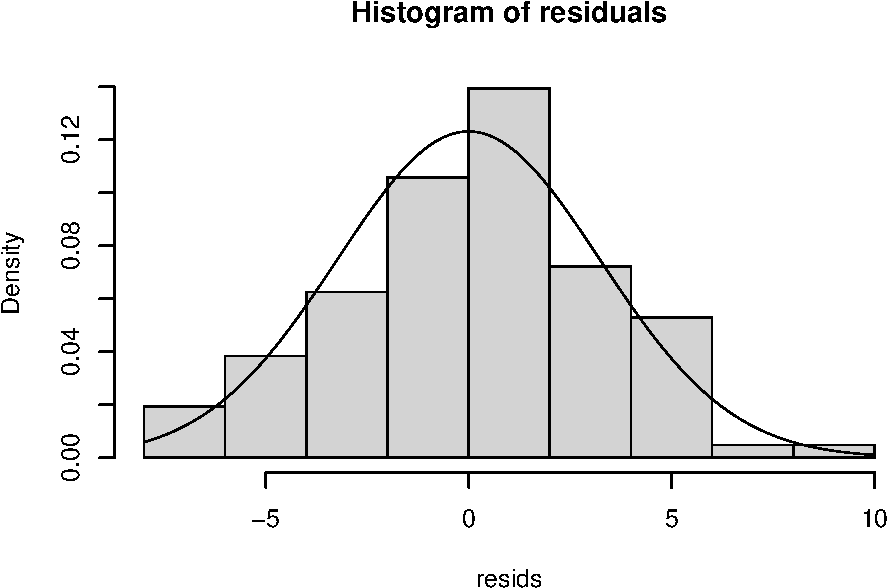
\includegraphics{phcm9795-solutions-R_files/figure-latex/unnamed-chunk-85-1.pdf}

\begin{enumerate}
\def\labelenumi{\alph{enumi})}
\setcounter{enumi}{4}
\tightlist
\item
  What could you infer about the association between age and IQ in the population, based on the results of the regression analysis in this sample?
\end{enumerate}

\begin{quote}
This study provides very strong evidence that IQ is negatively associated with age (t=--6.24 with 102 df, P\textless0.001). For every year increase in age, we predict a 0.423 unit decrease in IQ and we are 95\% confident that the true decrease in IQ lies between 0.289 to 0.558 units. Variability in age explains 27.6\% of the variability in IQ.
\end{quote}

\hypertarget{activity-8.3}{%
\subsection*{Activity 8.3}\label{activity-8.3}}
\addcontentsline{toc}{subsection}{Activity 8.3}

Which of the following correlation coefficients indicates the weakest relationship and why?
a) r=0.72
b) r=0.41
c) r=0.13
d) r = −0.33
e) r = −0.84

\begin{quote}
Answer: c.
\end{quote}

\begin{quote}
r = 0.13 which is closest to 0. Note that this only relates to the strength of a linear relationship.
\end{quote}

\hypertarget{activity-8.4}{%
\subsection*{Activity 8.4}\label{activity-8.4}}
\addcontentsline{toc}{subsection}{Activity 8.4}

Are the following statements true or false?

\begin{enumerate}
\def\labelenumi{\alph{enumi})}
\tightlist
\item
  If a correlation coefficient is closer to 1.00 than to 0.00, this indicates that the outcome is caused by the exposure.
\end{enumerate}

\begin{quote}
False: Correlation cannot tell you about causation; it can only tell you if a relationship or association exists between 2 variables.
\end{quote}

\begin{enumerate}
\def\labelenumi{\alph{enumi})}
\setcounter{enumi}{1}
\tightlist
\item
  If a researcher has data on two variables, there will be a higher correlation if the two means are close together and a lower correlation if the two means are far apart.
\end{enumerate}

\begin{quote}
False: Correlation is not determined by the means of the variables. Correlation only indicates whether the value of one variable increases as the value of the other variable increases or decreases (in a linear way).
\end{quote}

\hypertarget{module-8-full-script}{%
\chapter*{Module 8: Full script}\label{module-8-full-script}}
\addcontentsline{toc}{chapter}{Module 8: Full script}

\begin{Shaded}
\begin{Highlighting}[]
\CommentTok{\# Author: Timothy Dobbins}
\CommentTok{\# Date: July, 2022}
\CommentTok{\# Purpose: Learning activities for Module 8}

\CommentTok{\# Activity 8.1}
\NormalTok{iq }\OtherTok{\textless{}{-}} \FunctionTok{readRDS}\NormalTok{(}\StringTok{"data/activities/Activity\_S8.2.rds"}\NormalTok{)}

\FunctionTok{plot}\NormalTok{(iq}\SpecialCharTok{$}\NormalTok{age, iq}\SpecialCharTok{$}\NormalTok{iq, }
     \AttributeTok{main=}\StringTok{"Scatter plot of IQ against age"}\NormalTok{,}
     \AttributeTok{xlab =} \StringTok{"Age (years)"}\NormalTok{,}
     \AttributeTok{ylab =} \StringTok{"IQ"}\NormalTok{)}

\FunctionTok{abline}\NormalTok{(}\FunctionTok{lm}\NormalTok{(iq}\SpecialCharTok{$}\NormalTok{iq }\SpecialCharTok{\textasciitilde{}}\NormalTok{ iq}\SpecialCharTok{$}\NormalTok{age))}

\FunctionTok{cor.test}\NormalTok{(iq}\SpecialCharTok{$}\NormalTok{age, iq}\SpecialCharTok{$}\NormalTok{iq)}

\NormalTok{model }\OtherTok{\textless{}{-}} \FunctionTok{lm}\NormalTok{(iq}\SpecialCharTok{$}\NormalTok{iq }\SpecialCharTok{\textasciitilde{}}\NormalTok{ iq}\SpecialCharTok{$}\NormalTok{age)}
\FunctionTok{summary}\NormalTok{(model)}
\FunctionTok{confint}\NormalTok{(model)}

\NormalTok{resids }\OtherTok{\textless{}{-}} \FunctionTok{resid}\NormalTok{(model)}

\FunctionTok{hist}\NormalTok{(resids, }\AttributeTok{probability =}\ConstantTok{TRUE}\NormalTok{,}
     \AttributeTok{main =} \StringTok{"Histogram of residuals"}\NormalTok{)}
\FunctionTok{curve}\NormalTok{(}\FunctionTok{dnorm}\NormalTok{(x,}
            \AttributeTok{mean=}\FunctionTok{mean}\NormalTok{(resids),}
            \AttributeTok{sd=}\FunctionTok{sd}\NormalTok{(resids)), }\AttributeTok{add =} \ConstantTok{TRUE}\NormalTok{)}
\end{Highlighting}
\end{Shaded}

\hypertarget{module-9-solutions-to-learning-activities}{%
\chapter*{Module 9: Solutions to Learning Activities}\label{module-9-solutions-to-learning-activities}}
\addcontentsline{toc}{chapter}{Module 9: Solutions to Learning Activities}

\hypertarget{activity-9.1}{%
\subsection*{Activity 9.1}\label{activity-9.1}}
\addcontentsline{toc}{subsection}{Activity 9.1}

There is a hypothesis that university students who live and dine in the university hall consume less vitamin C than the students who live and dine at home. To test the hypothesis, 30 students were randomly selected and their urinary ascorbic acid level was measured in mg over 3 hours. Urinary excretion of ascorbic acid is a measure of vitamin C nutrition in humans. The data is given as ActivityS9.1.rds.

\begin{enumerate}
\def\labelenumi{\alph{enumi})}
\tightlist
\item
  Examine the distribution of the data using a box-plot and histogram.
\end{enumerate}

\begin{Shaded}
\begin{Highlighting}[]
\FunctionTok{library}\NormalTok{(jmv)}

\NormalTok{diet }\OtherTok{\textless{}{-}} \FunctionTok{readRDS}\NormalTok{(}\StringTok{"data/activities/Activity\_S9.1.rds"}\NormalTok{)}

\FunctionTok{head}\NormalTok{(diet)}
\end{Highlighting}
\end{Shaded}

\begin{verbatim}
##                        dint ascorb
## 1 Living and dining in hall      7
## 2 Living and dining at home     22
## 3 Living and dining in hall      9
## 4 Living and dining at home     25
## 5 Living and dining in hall     14
## 6 Living and dining at home     30
\end{verbatim}

\begin{Shaded}
\begin{Highlighting}[]
\NormalTok{hall }\OtherTok{\textless{}{-}} \FunctionTok{subset}\NormalTok{(diet, dint}\SpecialCharTok{==}\StringTok{"Living and dining in hall"}\NormalTok{)}
\NormalTok{home }\OtherTok{\textless{}{-}} \FunctionTok{subset}\NormalTok{(diet, dint}\SpecialCharTok{==}\StringTok{"Living and dining at home"}\NormalTok{)}

\CommentTok{\# Set the graphics parameters to plot 2 rows and 2 columns:}
\FunctionTok{par}\NormalTok{(}\AttributeTok{mfrow=}\FunctionTok{c}\NormalTok{(}\DecValTok{2}\NormalTok{,}\DecValTok{2}\NormalTok{))}

\CommentTok{\# Specify each plot separately}
\FunctionTok{hist}\NormalTok{(hall}\SpecialCharTok{$}\NormalTok{ascorb, }\AttributeTok{xlab=}\StringTok{"Ascorbic acid (mg / 3 hr)"}\NormalTok{,}
     \AttributeTok{xlim=}\FunctionTok{c}\NormalTok{(}\DecValTok{0}\NormalTok{, }\DecValTok{400}\NormalTok{), }\AttributeTok{main=}\StringTok{"Living and dining in hall"}\NormalTok{)}
\FunctionTok{hist}\NormalTok{(home}\SpecialCharTok{$}\NormalTok{ascorb, }\AttributeTok{xlab=}\StringTok{"Ascorbic acid (mg / 3 hr)"}\NormalTok{, }\AttributeTok{main=}\StringTok{"Living and dining at home"}\NormalTok{)}

\FunctionTok{boxplot}\NormalTok{(hall}\SpecialCharTok{$}\NormalTok{ascorb, }\AttributeTok{ylab=}\StringTok{"Ascorbic acid (mg / 3 hr)"}\NormalTok{, }
        \AttributeTok{ylim=}\FunctionTok{c}\NormalTok{(}\DecValTok{0}\NormalTok{, }\DecValTok{400}\NormalTok{), }\AttributeTok{main=}\StringTok{"Living and dining in hall"}\NormalTok{)}
\FunctionTok{boxplot}\NormalTok{(home}\SpecialCharTok{$}\NormalTok{ascorb, }\AttributeTok{ylab=}\StringTok{"Ascorbic acid (mg / 3 hr)"}\NormalTok{, }\AttributeTok{main=}\StringTok{"Living and dining at home"}\NormalTok{)}
\end{Highlighting}
\end{Shaded}

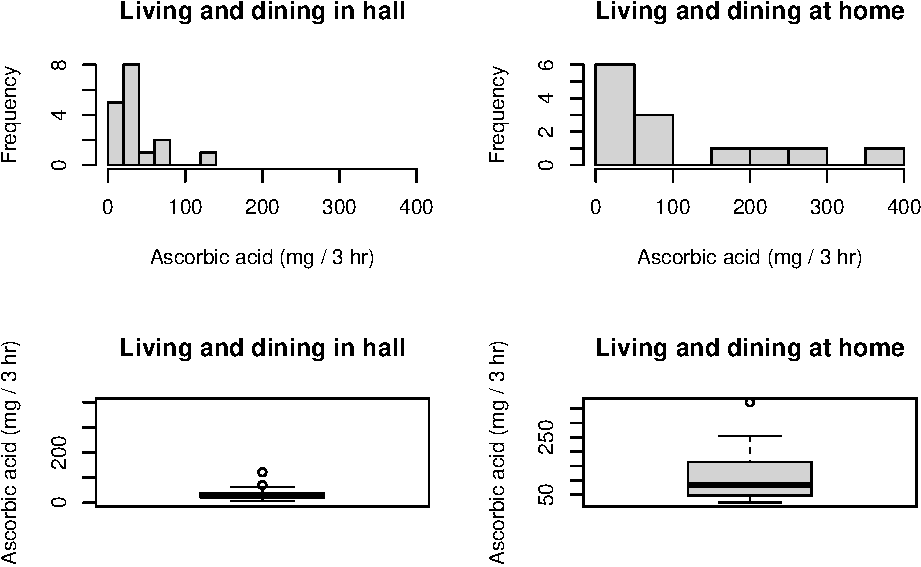
\includegraphics{phcm9795-solutions-R_files/figure-latex/unnamed-chunk-87-1.pdf}

\begin{Shaded}
\begin{Highlighting}[]
\FunctionTok{par}\NormalTok{(}\AttributeTok{mfrow=}\FunctionTok{c}\NormalTok{(}\DecValTok{1}\NormalTok{,}\DecValTok{1}\NormalTok{))}
\end{Highlighting}
\end{Shaded}

\begin{quote}
By examining the box plots and histograms we can say that ascorbic acid data for both of the student groups are highly positively skewed as well as highly peaked with some outliers that are biologically plausible.
\end{quote}

\begin{enumerate}
\def\labelenumi{\alph{enumi})}
\setcounter{enumi}{1}
\tightlist
\item
  Which statistical test would be appropriate to test the hypothesis mentioned in the question and why?
\end{enumerate}

\begin{quote}
Following the decision tree, the response variable is continuous (concentration of urinary ascorbic acid) and the explanatory variable is categorical (residential and dining status of the students) with two groups (binary). The two groups are independent as students either live at home or at university, not both. As evident from (a) the distribution of the response variable for both of the groups is highly positively skewed and peaked. Therefore, a distribution free (non-parametric) test would be appropriate to analyse the data. Because the distribution of both of the groups (Hall and Home) are positively skewed, that is they are of the same shape, the Wilcoxon rank-sum test would be appropriate to test the difference in medians.
\end{quote}

\begin{enumerate}
\def\labelenumi{\alph{enumi})}
\setcounter{enumi}{2}
\tightlist
\item
  State the hypothesis appropriate to the analytical method you mentioned in (b)?
\end{enumerate}

\begin{quote}
Null hypothesis: The median concentration of urinary ascorbic acid among the students who live and dine in the university hall is the same as that of the students who live and dine at home.
Alternative hypothesis: The median concentration of urinary ascorbic acid among the students who live and dine in the university hall is not same as that of the students who live and dine at home.
\end{quote}

\begin{enumerate}
\def\labelenumi{\alph{enumi})}
\setcounter{enumi}{3}
\tightlist
\item
  Use R to carry out the statistical test you have mentioned in (b) and write your conclusion.
\end{enumerate}

\begin{quote}
We can use the \texttt{wilcox.test()} function to carry out the Wilcoxon rank-sum test.
\end{quote}

\begin{Shaded}
\begin{Highlighting}[]
\FunctionTok{wilcox.test}\NormalTok{(ascorb }\SpecialCharTok{\textasciitilde{}}\NormalTok{ dint, }\AttributeTok{data=}\NormalTok{diet)}
\end{Highlighting}
\end{Shaded}

\begin{verbatim}
## Warning in wilcox.test.default(x = DATA[[1L]], y = DATA[[2L]], ...): cannot
## compute exact p-value with ties
\end{verbatim}

\begin{verbatim}
## 
##  Wilcoxon rank sum test with continuity correction
## 
## data:  ascorb by dint
## W = 45.5, p-value = 0.006927
## alternative hypothesis: true location shift is not equal to 0
\end{verbatim}

\begin{quote}
The P-value from the test is 0.007, which indicates that there is strong evidence of a difference between the median values of urinary ascorbic acid between the two student groups. The Wilcoxon rank-sum test does not report median values of the individual groups as part of the output. To include median values in the conclusion, we need to run the \texttt{descriptives()} command as shown below.
\end{quote}

\begin{Shaded}
\begin{Highlighting}[]
\FunctionTok{descriptives}\NormalTok{(}\AttributeTok{data=}\NormalTok{diet, }\AttributeTok{vars=}\NormalTok{ascorb, }\AttributeTok{splitBy =}\NormalTok{ dint,}
          \AttributeTok{pc=}\ConstantTok{TRUE}\NormalTok{)   }
\end{Highlighting}
\end{Shaded}

\begin{verbatim}
## 
##  DESCRIPTIVES
## 
##  Descriptives                                                    
##  ─────────────────────────────────────────────────────────────── 
##                          dint                         ascorb     
##  ─────────────────────────────────────────────────────────────── 
##    N                     Living and dining in hall          17   
##                          Living and dining at home          13   
##    Missing               Living and dining in hall           0   
##                          Living and dining at home           0   
##    Mean                  Living and dining in hall    36.64706   
##                          Living and dining at home    114.2308   
##    Median                Living and dining in hall    28.00000   
##                          Living and dining at home    83.00000   
##    Standard deviation    Living and dining in hall    27.91044   
##                          Living and dining at home    106.2302   
##    Minimum               Living and dining in hall    7.000000   
##                          Living and dining at home    22.00000   
##    Maximum               Living and dining in hall    121.0000   
##                          Living and dining at home    372.0000   
##    25th percentile       Living and dining in hall    20.00000   
##                          Living and dining at home    47.00000   
##    50th percentile       Living and dining in hall    28.00000   
##                          Living and dining at home    83.00000   
##    75th percentile       Living and dining in hall    38.00000   
##                          Living and dining at home    163.0000   
##  ───────────────────────────────────────────────────────────────
\end{verbatim}

\begin{quote}
\textbf{Conclusion:} There is strong evidence from Wilcoxon rank-sum test (P = 0.007) that the median concentration of urinary ascorbic acid among the university students who live and dine at home (83 mg per 3 hours, interquartile range: 47 to 163) is higher than that of the students who live and dine in the university hall (28 mg per 3 hours, interquartile range: 20 to 38).
\end{quote}

\hypertarget{activity-9.2}{%
\subsection*{Activity 9.2}\label{activity-9.2}}
\addcontentsline{toc}{subsection}{Activity 9.2}

A drug was tested for its effect in lowering blood pressure. Fifteen women with hypertension were enrolled and had their systolic blood pressure measured before and after taking the drug. The data are available in the file Activity\_S9.2.rds on Moodle.

\begin{enumerate}
\def\labelenumi{\alph{enumi})}
\tightlist
\item
  State the research question and the null hypothesis.
\end{enumerate}

\begin{quote}
Research question: Do women with hypertension have lower systolic blood pressure after taking the test drug than before taking the drug?
\end{quote}

\begin{quote}
Null hypothesis: There is no change in median systolic blood pressure before and after taking the drug.
\end{quote}

\begin{enumerate}
\def\labelenumi{\alph{enumi})}
\setcounter{enumi}{1}
\tightlist
\item
  Use R to obtain suitable summary statistics and test the null hypothesis. Describe the reason for choosing the test.
\end{enumerate}

\begin{quote}
Systolic blood pressure was measured for each person twice to compare the difference in blood pressure before and after taking the drug. Therefore, the study is a paired design and, because blood pressure is a continuous measurement, a paired t-test can be considered. One of the assumptions of a paired t-test is that the differences between the measurements are normally distributed and this needs to be checked.
\end{quote}

\begin{quote}
To check the distribution of the differences between the measurements, we first need to calculate the differences. We created a new variable `difference' using the equation `BP\_After\_mmHg − BP\_Before\_mmHg'. The histogram of the differences is shown in Figure 2.
\end{quote}

\begin{Shaded}
\begin{Highlighting}[]
\NormalTok{bp }\OtherTok{\textless{}{-}} \FunctionTok{readRDS}\NormalTok{(}\StringTok{"data/activities/Activity\_S9.2.rds"}\NormalTok{)}
\FunctionTok{head}\NormalTok{(bp)}
\end{Highlighting}
\end{Shaded}

\begin{verbatim}
##   id bp_before_mmhg bp_after_mmhg difference
## 1  1            143           120        -23
## 2  2            150           124        -26
## 3  3            140           130        -10
## 4  4            139           118        -21
## 5  5            141           140         -1
## 6  6            144           128        -16
\end{verbatim}

\begin{Shaded}
\begin{Highlighting}[]
\FunctionTok{hist}\NormalTok{(bp}\SpecialCharTok{$}\NormalTok{difference,}
     \AttributeTok{main=}\StringTok{"Figure 2: Reduction in blood pressure after taking a new drug"}\NormalTok{,}
     \AttributeTok{xlab=}\StringTok{"Difference (mmHg)"}\NormalTok{)}
\end{Highlighting}
\end{Shaded}

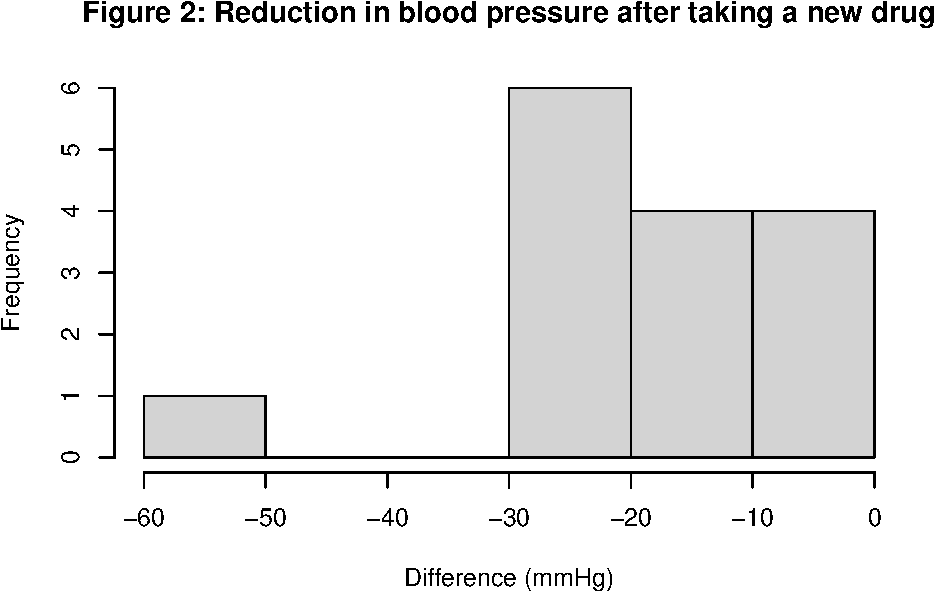
\includegraphics{phcm9795-solutions-R_files/figure-latex/unnamed-chunk-90-1.pdf}

\begin{Shaded}
\begin{Highlighting}[]
\CommentTok{\# Note {-} histogram differs from Stata, as R uses intervals as (a, b], where as Stata uses [a, b).}
\end{Highlighting}
\end{Shaded}

\begin{quote}
The histogram of the differences (BP\_After -- BP\_Before) does not approximate a normal distribution. Therefore, the paired t-test is not appropriate and its non-parametric equivalent, the Wilcoxon signed rank test, should be considered.
The Wilcoxon signed rank test is obtained using the \texttt{wilcox.test()} function:
\end{quote}

\begin{Shaded}
\begin{Highlighting}[]
\FunctionTok{wilcox.test}\NormalTok{(bp}\SpecialCharTok{$}\NormalTok{bp\_before\_mmhg, bp}\SpecialCharTok{$}\NormalTok{bp\_after\_mmhg, }\AttributeTok{paired=}\ConstantTok{TRUE}\NormalTok{)}
\end{Highlighting}
\end{Shaded}

\begin{verbatim}
## Warning in wilcox.test.default(bp$bp_before_mmhg, bp$bp_after_mmhg, paired =
## TRUE): cannot compute exact p-value with ties
\end{verbatim}

\begin{verbatim}
## 
##  Wilcoxon signed rank test with continuity correction
## 
## data:  bp$bp_before_mmhg and bp$bp_after_mmhg
## V = 120, p-value = 0.0007158
## alternative hypothesis: true location shift is not equal to 0
\end{verbatim}

\begin{enumerate}
\def\labelenumi{\alph{enumi})}
\setcounter{enumi}{2}
\tightlist
\item
  Write a brief conclusion.
\end{enumerate}

\begin{quote}
To include descriptive summary statistics in our conclusion we need to obtain summary statistics of the blood pressure measurements before and after taking the drug and the differences between these two measurements.
\end{quote}

\begin{Shaded}
\begin{Highlighting}[]
\FunctionTok{descriptives}\NormalTok{(}\AttributeTok{data=}\NormalTok{bp, }\AttributeTok{vars=}\FunctionTok{c}\NormalTok{(bp\_before\_mmhg, bp\_after\_mmhg, difference),}
             \AttributeTok{pc=}\ConstantTok{TRUE}\NormalTok{)}
\end{Highlighting}
\end{Shaded}

\begin{verbatim}
## 
##  DESCRIPTIVES
## 
##  Descriptives                                                            
##  ─────────────────────────────────────────────────────────────────────── 
##                          bp_before_mmhg    bp_after_mmhg    difference   
##  ─────────────────────────────────────────────────────────────────────── 
##    N                                 15               15            15   
##    Missing                            0                0             0   
##    Mean                        146.4667         129.2667     -17.20000   
##    Median                      144.0000         128.0000     -16.00000   
##    Standard deviation          10.75617         6.902036      13.41215   
##    Minimum                     139.0000         118.0000     -57.00000   
##    Maximum                     183.0000         140.0000     -1.000000   
##    25th percentile             140.5000         125.5000     -21.00000   
##    50th percentile             144.0000         128.0000     -16.00000   
##    75th percentile             146.5000         132.5000     -8.000000   
##  ───────────────────────────────────────────────────────────────────────
\end{verbatim}

\begin{quote}
The median (IQR) SBP before and after taking the drug was 144 (140 to 147) mmHg and 128 (125 to 135) mmHg, respectively. The median (IQR) reduction in SBP is 16 (6 to 21) mmHg. There is very strong evidence that the drug lowered blood pressure in this group of hypertensive women (Wilcoxon P = 0.0007).
\end{quote}

\begin{enumerate}
\def\labelenumi{\alph{enumi})}
\setcounter{enumi}{3}
\tightlist
\item
  What are the main limitations of this study? Consider both epidemiological and statistical aspects.
\end{enumerate}

\begin{quote}
The samples were selected from a small patient group with particular characteristics (hypertensive females). While the results may be generalisable to hypertensive women in the population, assuming the sample is representative of hypertensive women in the population, the results may not be applicable to men. The strongest weakness is that there is no control group; the blood pressure in the women may have in fact lowered in the absence of taking the drug. This could be avoided by conducting a randomised controlled trial.
\end{quote}

\hypertarget{module-9-full-script}{%
\chapter*{Module 9: Full script}\label{module-9-full-script}}
\addcontentsline{toc}{chapter}{Module 9: Full script}

\begin{Shaded}
\begin{Highlighting}[]
\CommentTok{\# Author: Timothy Dobbins}
\CommentTok{\# Date: July, 2022}
\CommentTok{\# Purpose: Learning activities for Module 9}

\CommentTok{\# Activity 9.1}
\FunctionTok{library}\NormalTok{(jmv)}

\NormalTok{diet }\OtherTok{\textless{}{-}} \FunctionTok{readRDS}\NormalTok{(}\StringTok{"data/activities/Activity\_S9.1.rds"}\NormalTok{)}

\FunctionTok{head}\NormalTok{(diet)}

\NormalTok{hall }\OtherTok{\textless{}{-}} \FunctionTok{subset}\NormalTok{(diet, dint}\SpecialCharTok{==}\StringTok{"Living and dining in hall"}\NormalTok{)}
\NormalTok{home }\OtherTok{\textless{}{-}} \FunctionTok{subset}\NormalTok{(diet, dint}\SpecialCharTok{==}\StringTok{"Living and dining at home"}\NormalTok{)}

\CommentTok{\# Set the graphics parameters to plot 2 rows and 2 columns:}
\FunctionTok{par}\NormalTok{(}\AttributeTok{mfrow=}\FunctionTok{c}\NormalTok{(}\DecValTok{2}\NormalTok{,}\DecValTok{2}\NormalTok{))}

\CommentTok{\# Specify each plot separately}
\FunctionTok{hist}\NormalTok{(hall}\SpecialCharTok{$}\NormalTok{ascorb, }\AttributeTok{xlab=}\StringTok{"Ascorbic acid (mg / 3 hr)"}\NormalTok{,}
     \AttributeTok{xlim=}\FunctionTok{c}\NormalTok{(}\DecValTok{0}\NormalTok{, }\DecValTok{400}\NormalTok{), }\AttributeTok{main=}\StringTok{"Living and dining in hall"}\NormalTok{)}
\FunctionTok{hist}\NormalTok{(home}\SpecialCharTok{$}\NormalTok{ascorb, }\AttributeTok{xlab=}\StringTok{"Ascorbic acid (mg / 3 hr)"}\NormalTok{, }\AttributeTok{main=}\StringTok{"Living and dining at home"}\NormalTok{)}

\FunctionTok{boxplot}\NormalTok{(hall}\SpecialCharTok{$}\NormalTok{ascorb, }\AttributeTok{ylab=}\StringTok{"Ascorbic acid (mg / 3 hr)"}\NormalTok{, }
        \AttributeTok{ylim=}\FunctionTok{c}\NormalTok{(}\DecValTok{0}\NormalTok{, }\DecValTok{400}\NormalTok{), }\AttributeTok{main=}\StringTok{"Living and dining in hall"}\NormalTok{)}
\FunctionTok{boxplot}\NormalTok{(home}\SpecialCharTok{$}\NormalTok{ascorb, }\AttributeTok{ylab=}\StringTok{"Ascorbic acid (mg / 3 hr)"}\NormalTok{, }\AttributeTok{main=}\StringTok{"Living and dining at home"}\NormalTok{)}

\FunctionTok{par}\NormalTok{(}\AttributeTok{mfrow=}\FunctionTok{c}\NormalTok{(}\DecValTok{1}\NormalTok{,}\DecValTok{1}\NormalTok{))}

\FunctionTok{wilcox.test}\NormalTok{(ascorb }\SpecialCharTok{\textasciitilde{}}\NormalTok{ dint, }\AttributeTok{data=}\NormalTok{diet)}

\FunctionTok{descriptives}\NormalTok{(}\AttributeTok{data=}\NormalTok{diet, }\AttributeTok{vars=}\NormalTok{ascorb, }\AttributeTok{splitBy =}\NormalTok{ dint,}
          \AttributeTok{pc=}\ConstantTok{TRUE}\NormalTok{)   }


\CommentTok{\# Activity 9.2}
\NormalTok{bp }\OtherTok{\textless{}{-}} \FunctionTok{readRDS}\NormalTok{(}\StringTok{"data/activities/Activity\_S9.2.rds"}\NormalTok{)}
\FunctionTok{head}\NormalTok{(bp)}

\FunctionTok{hist}\NormalTok{(bp}\SpecialCharTok{$}\NormalTok{difference,}
     \AttributeTok{main=}\StringTok{"Figure 2: Reduction in blood pressure after taking a new drug"}\NormalTok{,}
     \AttributeTok{xlab=}\StringTok{"Difference (mmHg)"}\NormalTok{)}
\CommentTok{\# Note {-} histogram differs from Stata, as R uses intervals as (a, b], where as Stata uses [a, b).}

\FunctionTok{wilcox.test}\NormalTok{(bp}\SpecialCharTok{$}\NormalTok{bp\_before\_mmhg, bp}\SpecialCharTok{$}\NormalTok{bp\_after\_mmhg, }\AttributeTok{paired=}\ConstantTok{TRUE}\NormalTok{)}
\FunctionTok{descriptives}\NormalTok{(}\AttributeTok{data=}\NormalTok{bp, }\AttributeTok{vars=}\FunctionTok{c}\NormalTok{(bp\_before\_mmhg, bp\_after\_mmhg, difference),}
             \AttributeTok{pc=}\ConstantTok{TRUE}\NormalTok{)}
\end{Highlighting}
\end{Shaded}

\hypertarget{module-10-solutions-to-learning-activities}{%
\chapter*{Module 10: Solutions to Learning Activities}\label{module-10-solutions-to-learning-activities}}
\addcontentsline{toc}{chapter}{Module 10: Solutions to Learning Activities}

\hypertarget{activity-10.1}{%
\subsection*{Activity 10.1}\label{activity-10.1}}
\addcontentsline{toc}{subsection}{Activity 10.1}

We are planning a study to measure the prevalence of a relatively rare condition (say approximately 5\%) in children aged 0-5 years in a remote community.

\begin{enumerate}
\def\labelenumi{\alph{enumi})}
\tightlist
\item
  What type of study would need to be conducted?
\end{enumerate}

\begin{quote}
A cross sectional survey where a sample of children aged 0-5 yrs will be randomly selected from the population.
\end{quote}

\begin{enumerate}
\def\labelenumi{\alph{enumi})}
\setcounter{enumi}{1}
\tightlist
\item
  Use the correct sample size table included in your notes to determine how many children would need to be enrolled for the confidence interval to be (i) 2\% (ii) 4\% around the prevalence? What would the resulting prevalence estimates and 95\% CIs be?
\end{enumerate}

\begin{quote}
We can use Table 10.1 in Module 10 to estimate the sample size.
\end{quote}

\begin{quote}
\begin{enumerate}
\def\labelenumi{\roman{enumi})}
\tightlist
\item
  If the prevalence in the population is 5\%, we will need 457 participants to estimate the 95\% CI with 2\% width. The resulting 95\% CI would be 3\% to 7\%.
\item
  If the prevalence in the population is 5\%, we will need 115 participants to estimate the 95\% CI with 4\% width. The resulting 95\% CI would be 1\% to 9\%.
\end{enumerate}
\end{quote}

\hypertarget{activity-10.2}{%
\subsection*{Activity 10.2}\label{activity-10.2}}
\addcontentsline{toc}{subsection}{Activity 10.2}

We are planning an experimental study to test the use of a new drug to alleviate the symptoms of the common cold compared to the use of Vitamin C. Participants will be randomised to receive the new experimental drug or to receive Vitamin C. How many participants will be required in each group (power = 80\%, level of significance = 5\%).

\begin{enumerate}
\def\labelenumi{\alph{enumi})}
\tightlist
\item
  If the resolution of symptoms is 10\% in the control group and 40\% in the new treatment group?
\end{enumerate}

\begin{quote}
We can use the \texttt{epi.sscohortc()} function to estimate the sample size, specifying the resolution rate in the control group (10\%, or 0.1), the resolution rate in the exposed group (40\%, or 0.4) and the power of 80\% (or 0.8):
\end{quote}

\begin{Shaded}
\begin{Highlighting}[]
\FunctionTok{library}\NormalTok{(epiR)}
\end{Highlighting}
\end{Shaded}

\begin{verbatim}
## Loading required package: survival
\end{verbatim}

\begin{verbatim}
## 
## Attaching package: 'survival'
\end{verbatim}

\begin{verbatim}
## The following object is masked _by_ '.GlobalEnv':
## 
##     heart
\end{verbatim}

\begin{verbatim}
## Package epiR 2.0.46 is loaded
\end{verbatim}

\begin{verbatim}
## Type help(epi.about) for summary information
\end{verbatim}

\begin{verbatim}
## Type browseVignettes(package = 'epiR') to learn how to use epiR for applied epidemiological analyses
\end{verbatim}

\begin{verbatim}
## 
\end{verbatim}

\begin{Shaded}
\begin{Highlighting}[]
\FunctionTok{epi.sscohortc}\NormalTok{(}\AttributeTok{irexp1=}\FloatTok{0.4}\NormalTok{, }\AttributeTok{irexp0=}\FloatTok{0.1}\NormalTok{, }\AttributeTok{n=}\ConstantTok{NA}\NormalTok{, }\AttributeTok{power=}\FloatTok{0.8}\NormalTok{)}
\end{Highlighting}
\end{Shaded}

\begin{verbatim}
## $n.total
## [1] 64
## 
## $n.exp1
## [1] 32
## 
## $n.exp0
## [1] 32
## 
## $power
## [1] 0.8
## 
## $irr
## [1] 4
## 
## $or
## [1] 6
\end{verbatim}

Here we see we require 32 in each group, or 64 particpants in total.

\begin{enumerate}
\def\labelenumi{\alph{enumi})}
\setcounter{enumi}{1}
\tightlist
\item
  How large will the sample size need to be if we decide to recruit two control participants to every intervention group participant?
\end{enumerate}

\begin{quote}
We can specify \texttt{r} in the \texttt{epi.sscohortc()} function which is specified as the number in the exposed group divided by the number in the unexposed group. If we want two control participants for every intervention participant, r=0.5:
\end{quote}

\begin{Shaded}
\begin{Highlighting}[]
\FunctionTok{epi.sscohortc}\NormalTok{(}\AttributeTok{irexp1=}\FloatTok{0.4}\NormalTok{, }\AttributeTok{irexp0=}\FloatTok{0.1}\NormalTok{, }\AttributeTok{r=}\FloatTok{0.5}\NormalTok{, }\AttributeTok{n=}\ConstantTok{NA}\NormalTok{, }\AttributeTok{power=}\FloatTok{0.8}\NormalTok{)}
\end{Highlighting}
\end{Shaded}

\begin{verbatim}
## $n.total
## [1] 67.5
## 
## $n.exp1
## [1] 22.5
## 
## $n.exp0
## [1] 45
## 
## $power
## [1] 0.8
## 
## $irr
## [1] 4
## 
## $or
## [1] 6
\end{verbatim}

\begin{quote}
For this situation, we are advised that we will need 22.5 participants in the intervention group and 45 in the control group, with total of 67.5 participants. Note that R has calculated that sample size in the exposed group as 0.5 times the control group. \textbf{If there is a decimal in any calculated sample size it should always be rounded up.}
\end{quote}

\begin{quote}
Thus, we require 23 participants in the intervention group and 45 in the control group, with total of 68 participants.
\end{quote}

\begin{enumerate}
\def\labelenumi{\alph{enumi})}
\setcounter{enumi}{2}
\tightlist
\item
  If we decide to retain a 1:1 ratio of participants in the intervention and controls groups but the resolution of symptoms is 20\% in the control group and 40\% in the new treatment group?
\end{enumerate}

\begin{Shaded}
\begin{Highlighting}[]
\FunctionTok{epi.sscohortc}\NormalTok{(}\AttributeTok{irexp1=}\FloatTok{0.4}\NormalTok{, }\AttributeTok{irexp0=}\FloatTok{0.2}\NormalTok{, }\AttributeTok{n=}\ConstantTok{NA}\NormalTok{, }\AttributeTok{power=}\FloatTok{0.8}\NormalTok{)}
\end{Highlighting}
\end{Shaded}

\begin{verbatim}
## $n.total
## [1] 164
## 
## $n.exp1
## [1] 82
## 
## $n.exp0
## [1] 82
## 
## $power
## [1] 0.8
## 
## $irr
## [1] 2
## 
## $or
## [1] 2.666667
\end{verbatim}

\begin{quote}
We will need 82 participants in each group.
\end{quote}

\begin{enumerate}
\def\labelenumi{\alph{enumi})}
\setcounter{enumi}{3}
\tightlist
\item
  How many participants would we need to recruit (calculated in c) if a pilot study shows that 15\% of people find the new treatment unpalatable and therefore do not take it?
\end{enumerate}

\begin{quote}
To accommodate 15\% noncompliance in the treatment group, the study team would need to recruit 15\% more in this group. That is 82/(1 − 0.15) = 82/0.85 = 96.47059, or 97 after rounding this number up. Thus, 97 participants should be recruited in the treatment group. Hence, the required total sample size would be 97 + 82 = 179 participants.
\end{quote}

\hypertarget{activity-10.3}{%
\subsection*{Activity 10.3}\label{activity-10.3}}
\addcontentsline{toc}{subsection}{Activity 10.3}

In a case-control study, we plan to recruit adult males who have been exposed to fumes from an industrial stack near their home and a sample of population controls in whom we expect that 20\% may also have been exposed to similar fumes through their place of residence or their work. We want to show that an odds ratio of 2.5 for having respiratory symptoms associated with exposure to fumes is statistically significant.

\begin{enumerate}
\def\labelenumi{\alph{enumi})}
\tightlist
\item
  What statistical test will be needed to measure the association between exposure and outcome?
\end{enumerate}

\begin{quote}
In this study, the outcome variable is dichotomous (case vs.~control) and the explanatory variable is also dichotomous (exposed vs.~unexposed). Therefore, a Pearson chi-squared test would be appropriate to assess the significance of the association.
\end{quote}

\begin{enumerate}
\def\labelenumi{\alph{enumi})}
\setcounter{enumi}{1}
\tightlist
\item
  How large will the sample size need to be to show that the OR of 2.5 is statistically significant at P \textless{} 0.05 with 90\% power if we want to recruit equal number of cases and controls?
\end{enumerate}

\begin{quote}
The proportion of the control group expected to be exposed to the study factor (explanatory variable) is 20\% and the required minimum detectable OR is 2.5. In the \texttt{epi.sscc()} function, we enter 0.2 as p0, 2.5 as the odds ratio to be detected and 0.9 as the power:
\end{quote}

\begin{Shaded}
\begin{Highlighting}[]
\FunctionTok{epi.sscc}\NormalTok{(}\AttributeTok{OR=}\FloatTok{2.5}\NormalTok{, }\AttributeTok{p0=}\FloatTok{0.2}\NormalTok{, }\AttributeTok{n=}\ConstantTok{NA}\NormalTok{, }\AttributeTok{power=}\FloatTok{0.9}\NormalTok{)}
\end{Highlighting}
\end{Shaded}

\begin{verbatim}
## $n.total
## [1] 252
## 
## $n.case
## [1] 126
## 
## $n.control
## [1] 126
## 
## $power
## [1] 0.9
## 
## $OR
## [1] 2.5
\end{verbatim}

\begin{quote}
The required sample is 126 cases and 126 controls, in total 252 participants.
\end{quote}

\begin{enumerate}
\def\labelenumi{\alph{enumi})}
\setcounter{enumi}{2}
\tightlist
\item
  What would be the required sample size (calculated in b) if the minimum detectable OR were 1.5?
\end{enumerate}

\begin{quote}
The required sample size has increased to 716 cases and 716 controls; in total 1432 participants:
\end{quote}

\begin{Shaded}
\begin{Highlighting}[]
\FunctionTok{epi.sscc}\NormalTok{(}\AttributeTok{OR=}\FloatTok{1.5}\NormalTok{, }\AttributeTok{p0=}\FloatTok{0.2}\NormalTok{, }\AttributeTok{n=}\ConstantTok{NA}\NormalTok{, }\AttributeTok{power=}\FloatTok{0.9}\NormalTok{)}
\end{Highlighting}
\end{Shaded}

\begin{verbatim}
## $n.total
## [1] 1432
## 
## $n.case
## [1] 716
## 
## $n.control
## [1] 716
## 
## $power
## [1] 0.9
## 
## $OR
## [1] 1.5
\end{verbatim}

\begin{enumerate}
\def\labelenumi{\alph{enumi})}
\setcounter{enumi}{3}
\tightlist
\item
  If there are problems recruiting cases to detect an OR of 1.5 (as calculated in c), what would the sample size need to be if the ratio of cases to controls was increased to 1:3?
\end{enumerate}

\begin{quote}
As in Question (1), 3 controls per case gives a ratio of 1/3 (=0.3333):
\end{quote}

\begin{Shaded}
\begin{Highlighting}[]
\FunctionTok{epi.sscc}\NormalTok{(}\AttributeTok{OR=}\FloatTok{1.5}\NormalTok{, }\AttributeTok{p0=}\FloatTok{0.2}\NormalTok{, }\AttributeTok{n=}\ConstantTok{NA}\NormalTok{, }\AttributeTok{power=}\FloatTok{0.9}\NormalTok{, }\AttributeTok{r=}\DecValTok{1}\SpecialCharTok{/}\DecValTok{3}\NormalTok{)}
\end{Highlighting}
\end{Shaded}

\begin{verbatim}
## $n.total
## [1] 1883
## 
## $n.case
## [1] 1412
## 
## $n.control
## [1] 471
## 
## $power
## [1] 0.9
## 
## $OR
## [1] 1.5
\end{verbatim}

The output shows that we will require 471 cases and 1412 controls for the study. In total 471 + 1412 = 1883 participants.

\hypertarget{activity-10.4}{%
\subsection*{Activity 10.4}\label{activity-10.4}}
\addcontentsline{toc}{subsection}{Activity 10.4}

In the above study to measure the effects of exposure to fumes from an industrial stack, we also want to know if the stack has an effect on lung function which can be measured as forced vital capacity in 1 minute (FEV1). This measurement is normally distributed in the population.

\begin{enumerate}
\def\labelenumi{\alph{enumi})}
\tightlist
\item
  If the research question is changed to wanting to show that the mean FEV1 in the exposed group is lower than the mean FEV1 in the control group what statistical test will now be required?
\end{enumerate}

\begin{quote}
An independent samples t-test because FEV1 is a normally distributed continuous variable, which will be compared between two independent groups (exposed and not exposed to industrial fumes).
\end{quote}

\begin{enumerate}
\def\labelenumi{\alph{enumi})}
\setcounter{enumi}{1}
\tightlist
\item
  Population statistics show that the mean FEV1 and its SD in the general population for males are 4.40 L (SD = 1.25) which can be expected in the control group. We expect that the mean FEV1 in the cases may be 4.0 L. How many participants will be needed to show that this mean value is significantly different from the control group with P \textless{} 0.05 with an 80\% power if we want to recruit equal number in each group?
\end{enumerate}

\begin{quote}
The given information should be entered into the \texttt{epi.sscompc()} function in the following way:
\end{quote}

\begin{Shaded}
\begin{Highlighting}[]
\FunctionTok{epi.sscompc}\NormalTok{(}\AttributeTok{treat =} \FloatTok{4.0}\NormalTok{, }\AttributeTok{control =} \FloatTok{4.4}\NormalTok{, }\AttributeTok{n =} \ConstantTok{NA}\NormalTok{, }\AttributeTok{sigma =} \FloatTok{1.25}\NormalTok{, }\AttributeTok{power =} \FloatTok{0.8}\NormalTok{)}
\end{Highlighting}
\end{Shaded}

\begin{verbatim}
## $n.total
## [1] 308
## 
## $n.treat
## [1] 154
## 
## $n.control
## [1] 154
## 
## $power
## [1] 0.8
## 
## $delta
## [1] 0.4
\end{verbatim}

\begin{quote}
We will require 154 participants to be recruited in each group to see the desired difference at 5\% significance level with 80\% power. (Note this solution is slightly different from Stata, which requires 155 participants in each group).
\end{quote}

\begin{enumerate}
\def\labelenumi{\alph{enumi})}
\setcounter{enumi}{2}
\tightlist
\item
  How much larger will the sample size need to be if the mean FEV1 in the cases is 4.20 L?
\end{enumerate}

\begin{Shaded}
\begin{Highlighting}[]
\FunctionTok{epi.sscompc}\NormalTok{(}\AttributeTok{treat =} \FloatTok{4.2}\NormalTok{, }\AttributeTok{control =} \FloatTok{4.4}\NormalTok{, }\AttributeTok{n =} \ConstantTok{NA}\NormalTok{, }\AttributeTok{sigma =} \FloatTok{1.25}\NormalTok{, }\AttributeTok{power =} \FloatTok{0.8}\NormalTok{)}
\end{Highlighting}
\end{Shaded}

\begin{verbatim}
## $n.total
## [1] 1228
## 
## $n.treat
## [1] 614
## 
## $n.control
## [1] 614
## 
## $power
## [1] 0.8
## 
## $delta
## [1] 0.2
\end{verbatim}

\begin{quote}
Changing the Experimental mean to 4.2 yields a required 614 participants in each group. (Note this solution is slightly different from Stata, which requires 615 participants in each group).
\end{quote}

\end{document}
